% !TeX spellcheck = en_US
\documentclass[]{scrartcl}

\usepackage{graphicx}
\usepackage{amsmath}
\usepackage{hyperref}
\usepackage{comment}
%opening
\title{Lab 3}
\author{}

\begin{document}

\maketitle

\begin{abstract}

\end{abstract}

\section{R1. Observation of the corrupted signal}\label{sec:R1}

\subsection{R1.a) Original sound file}
First of all the signal from the sound file \texttt{fugee.wav} was loaded and heard. It is the song \textit{Killing Me Softly With His Song} by \textit{Fugees}. Furthermore, sharp impulsive noise is heard at particular time instants, which simulates the noise that typically corrupts old vinyl records.

\subsection{R1.b) Time domain analysis of original signal}
Second, the sound signal is analyzed in the time domain. Fig. \ref{fig:R1b} shows the evolution of the a segment of signal with time. The sharp impulsive noise heard and described in the previous section is very noticeable in this figure. The noise seems to be modeled by an impulse.
\begin{figure}[htbp]
	\centering
	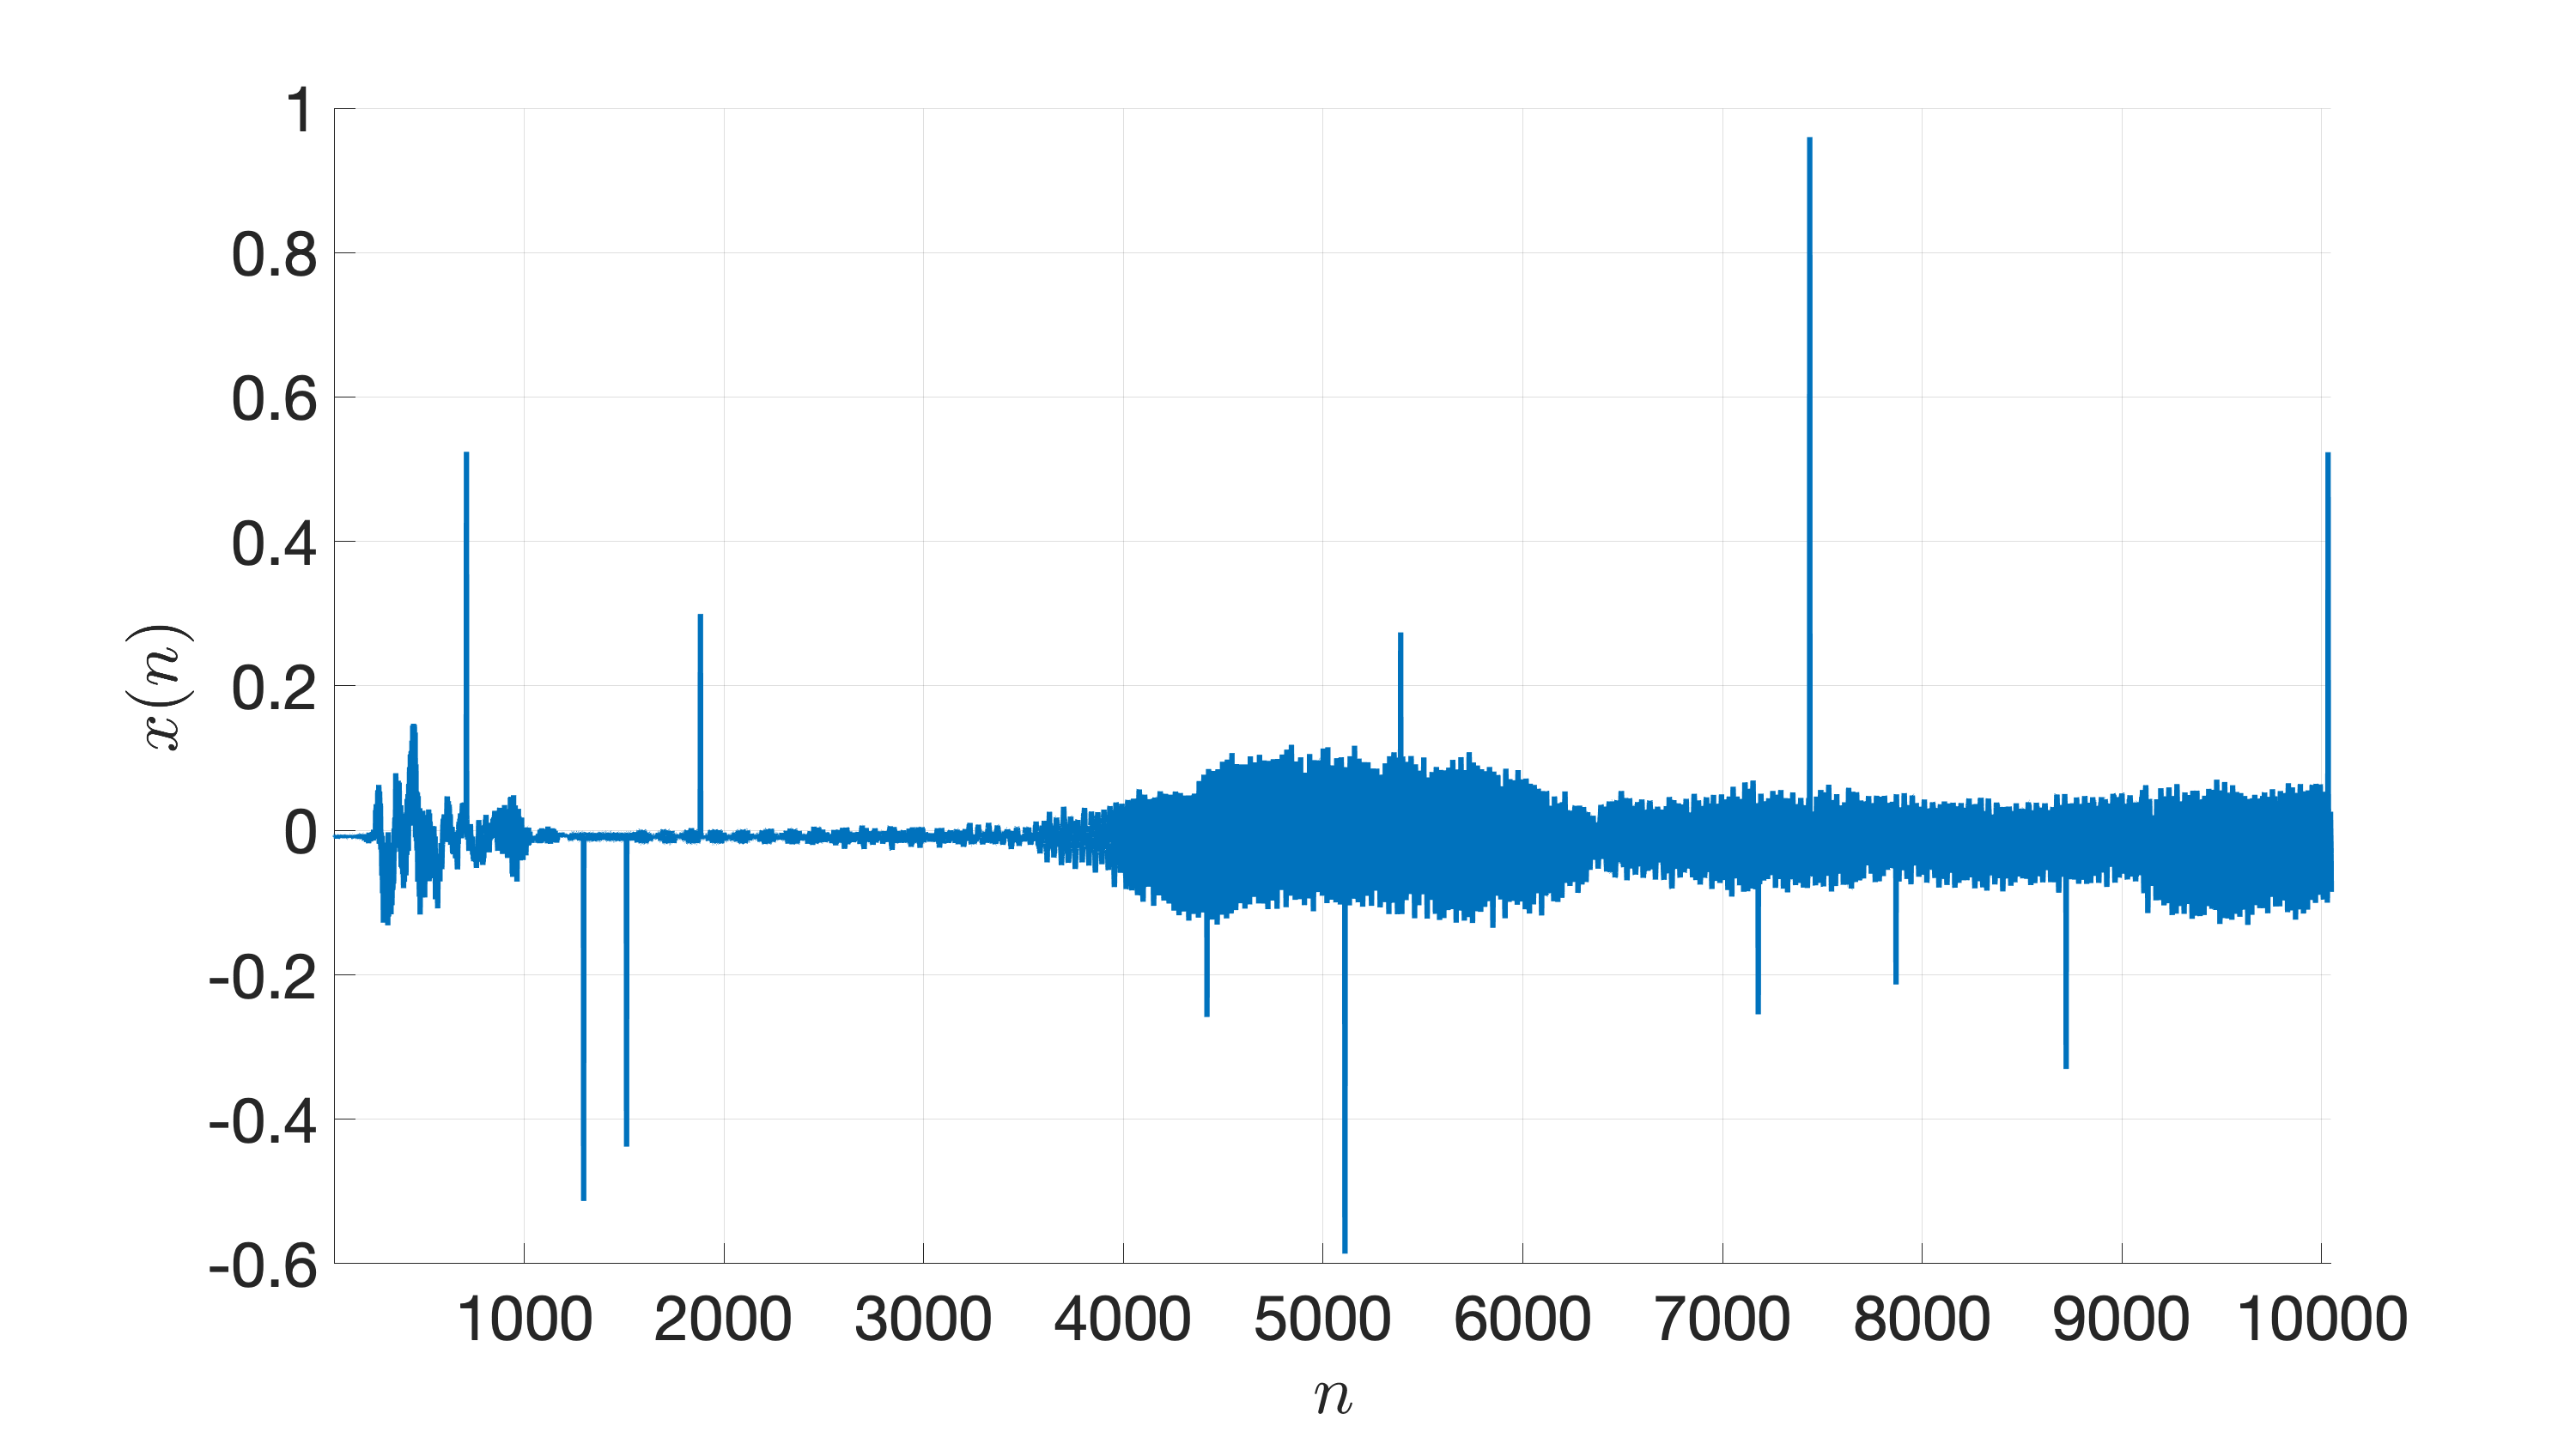
\includegraphics[width= 0.8\textwidth]{figures/R1b.png}
	\caption{Segment of the original sound signal in the time domain.}
	\label{fig:R1b}
\end{figure}

\subsection{R1.c) Frequency domain analysis of original signal}
Third, the sound signal is analyzed in the frequency domain. Fig. \ref{fig:R1c} shows the magnitude spectrum of the original signal. It shows the original sound signal has a broad frequency spectrum. Nevertheless, there is not clear evidence about the presence of noise in this plot. In fact, given that the noise is impulsive, its magnitude representation is a constant, thus very difficult to detect when superimposed with the spectrum of the song. As a matter of fact, the spectrogram of the segment of the sound plotted in Fig. \ref{fig:R1b} is shown in Fig. \ref{fig:R1c_spectrogram}. It is possible to notice that, as predicted, the instants for which there is impulsive noise correspond to a a constant spectrum across all frequencies. It is concluded that, while it is very easy to identify impulsive noise in the time domain, the opposite happens in the frequency domain. This fact hints that a filter suitable to filter such noise should operate in the time domain instead of the frequency domain.
\begin{comment}
\begin{figure}[htbp]
	\centering
	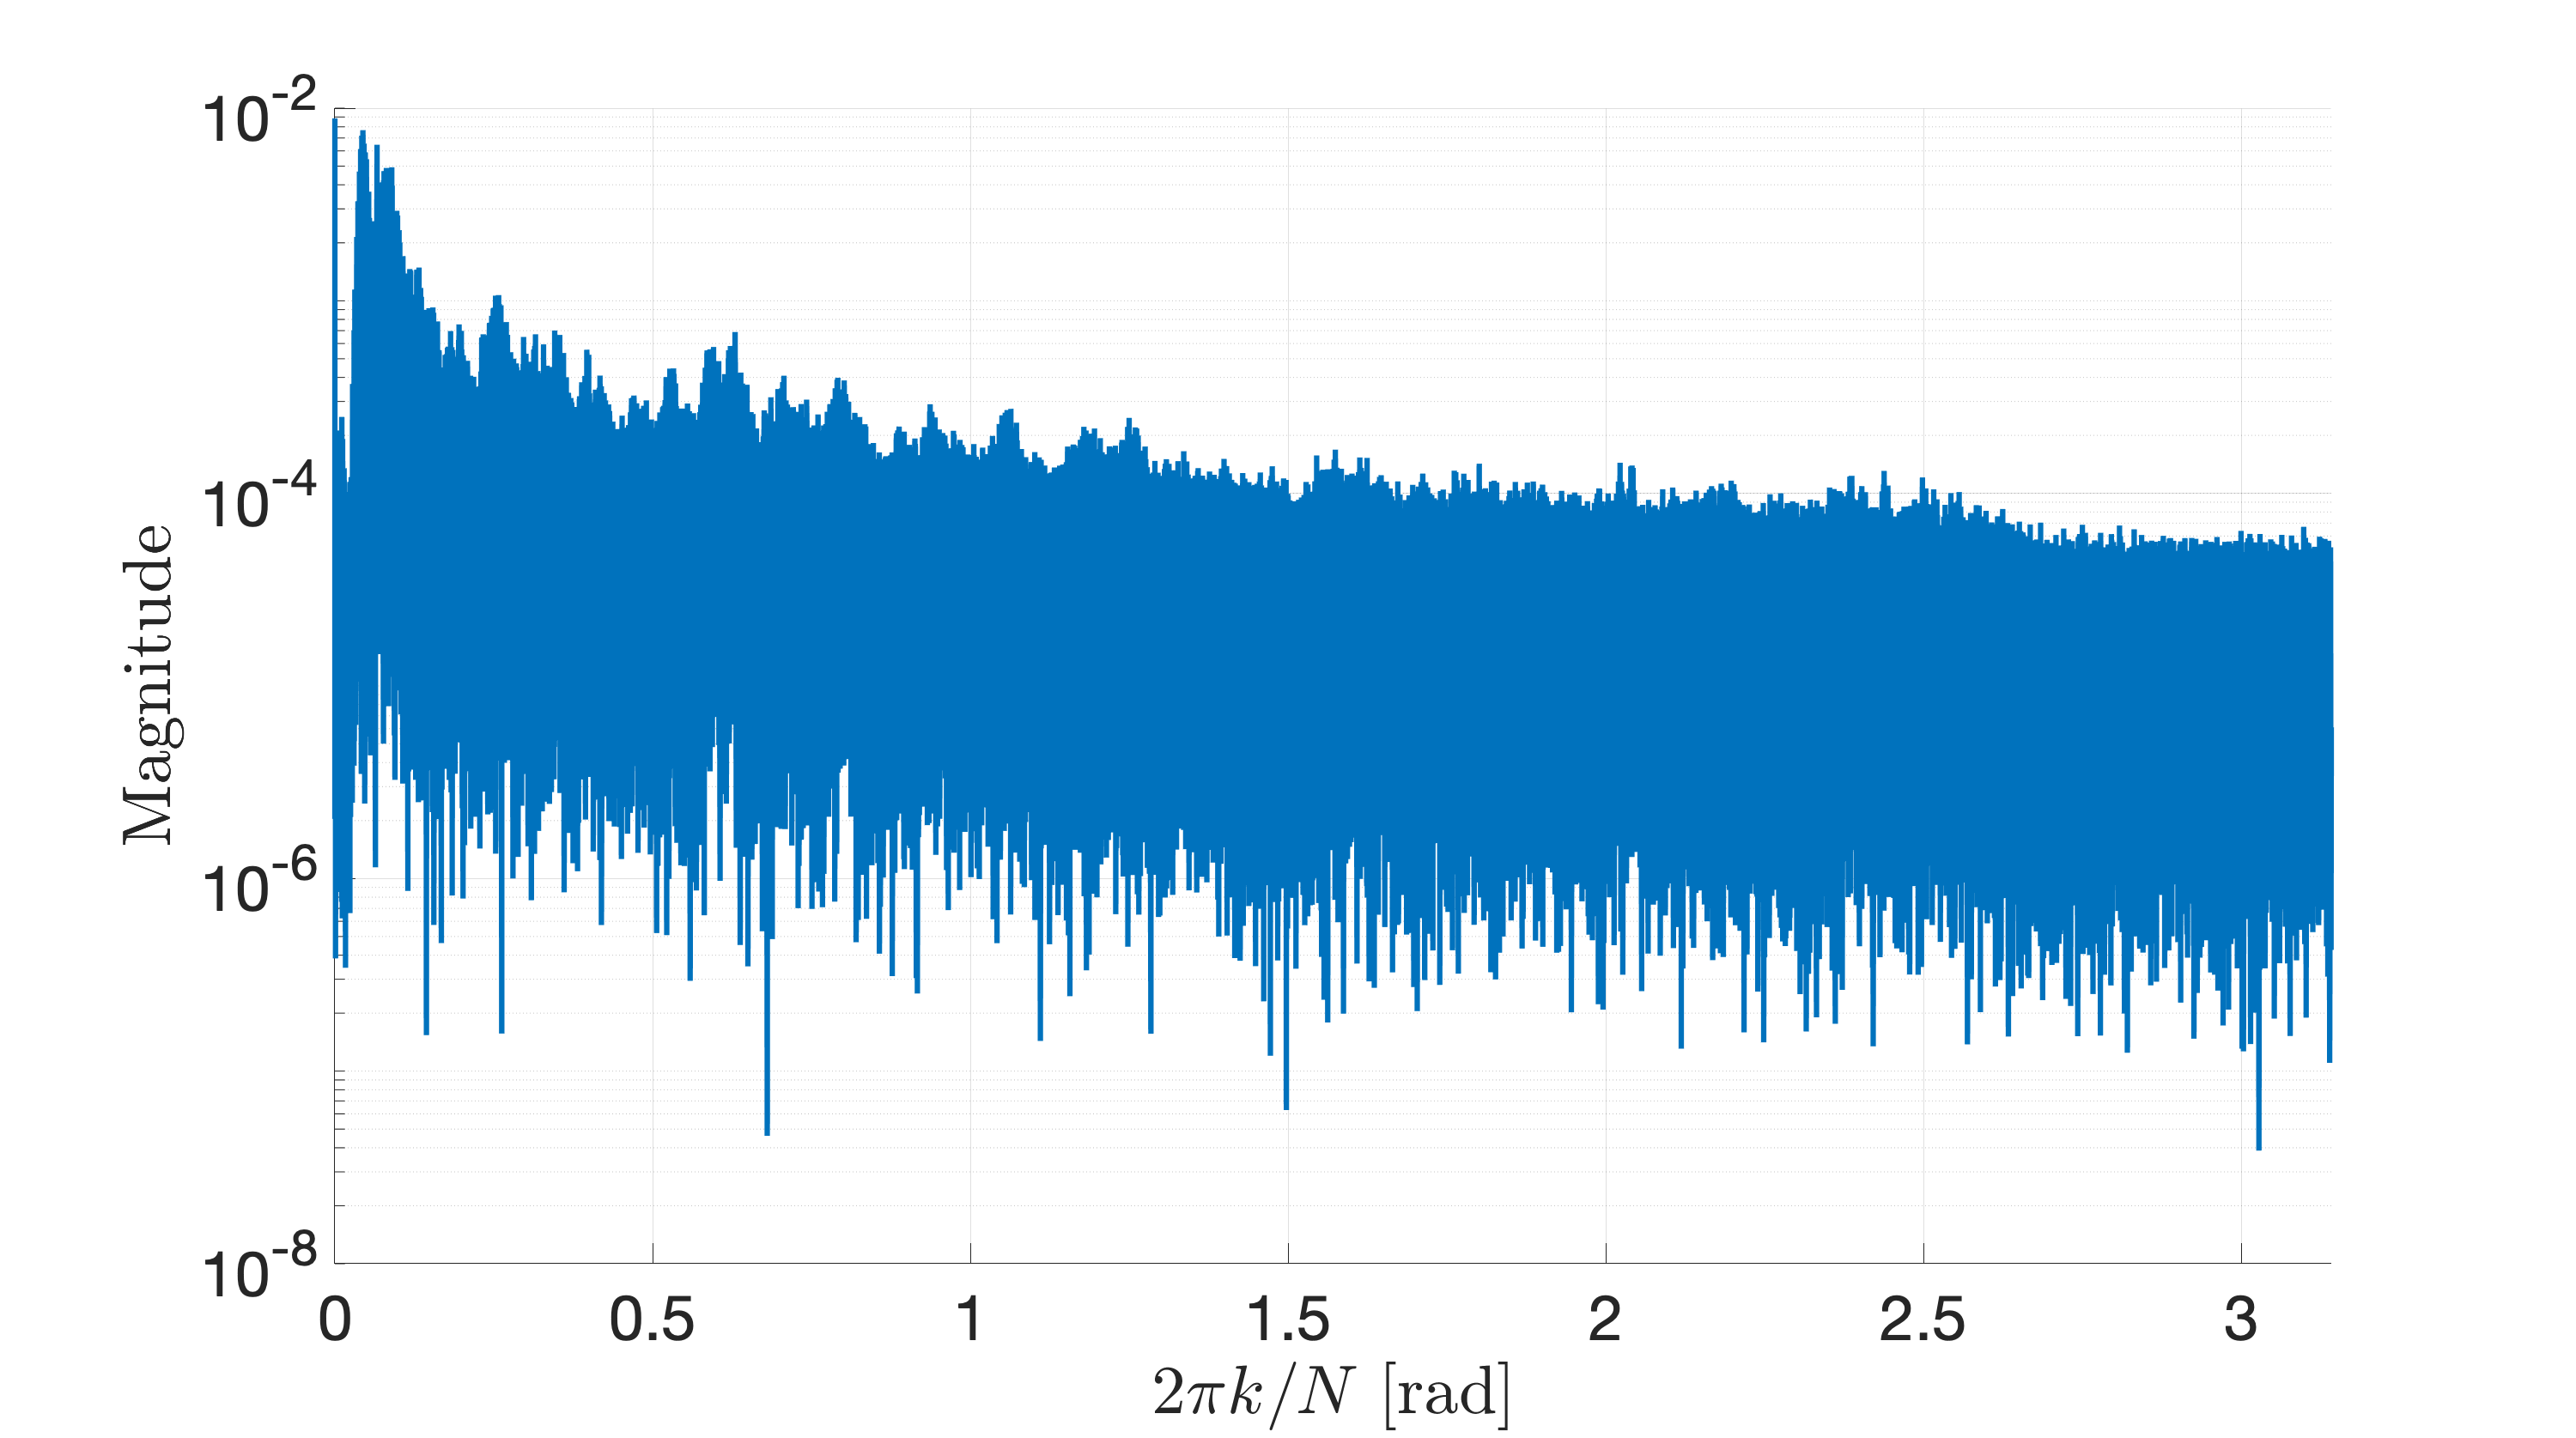
\includegraphics[width= 0.8\textwidth]{figures/R1c.png}
	\caption{Magnitude spectrum of the original sound signal.}
	\label{fig:R1c}
\end{figure}
\begin{figure}[htbp]
	\centering
	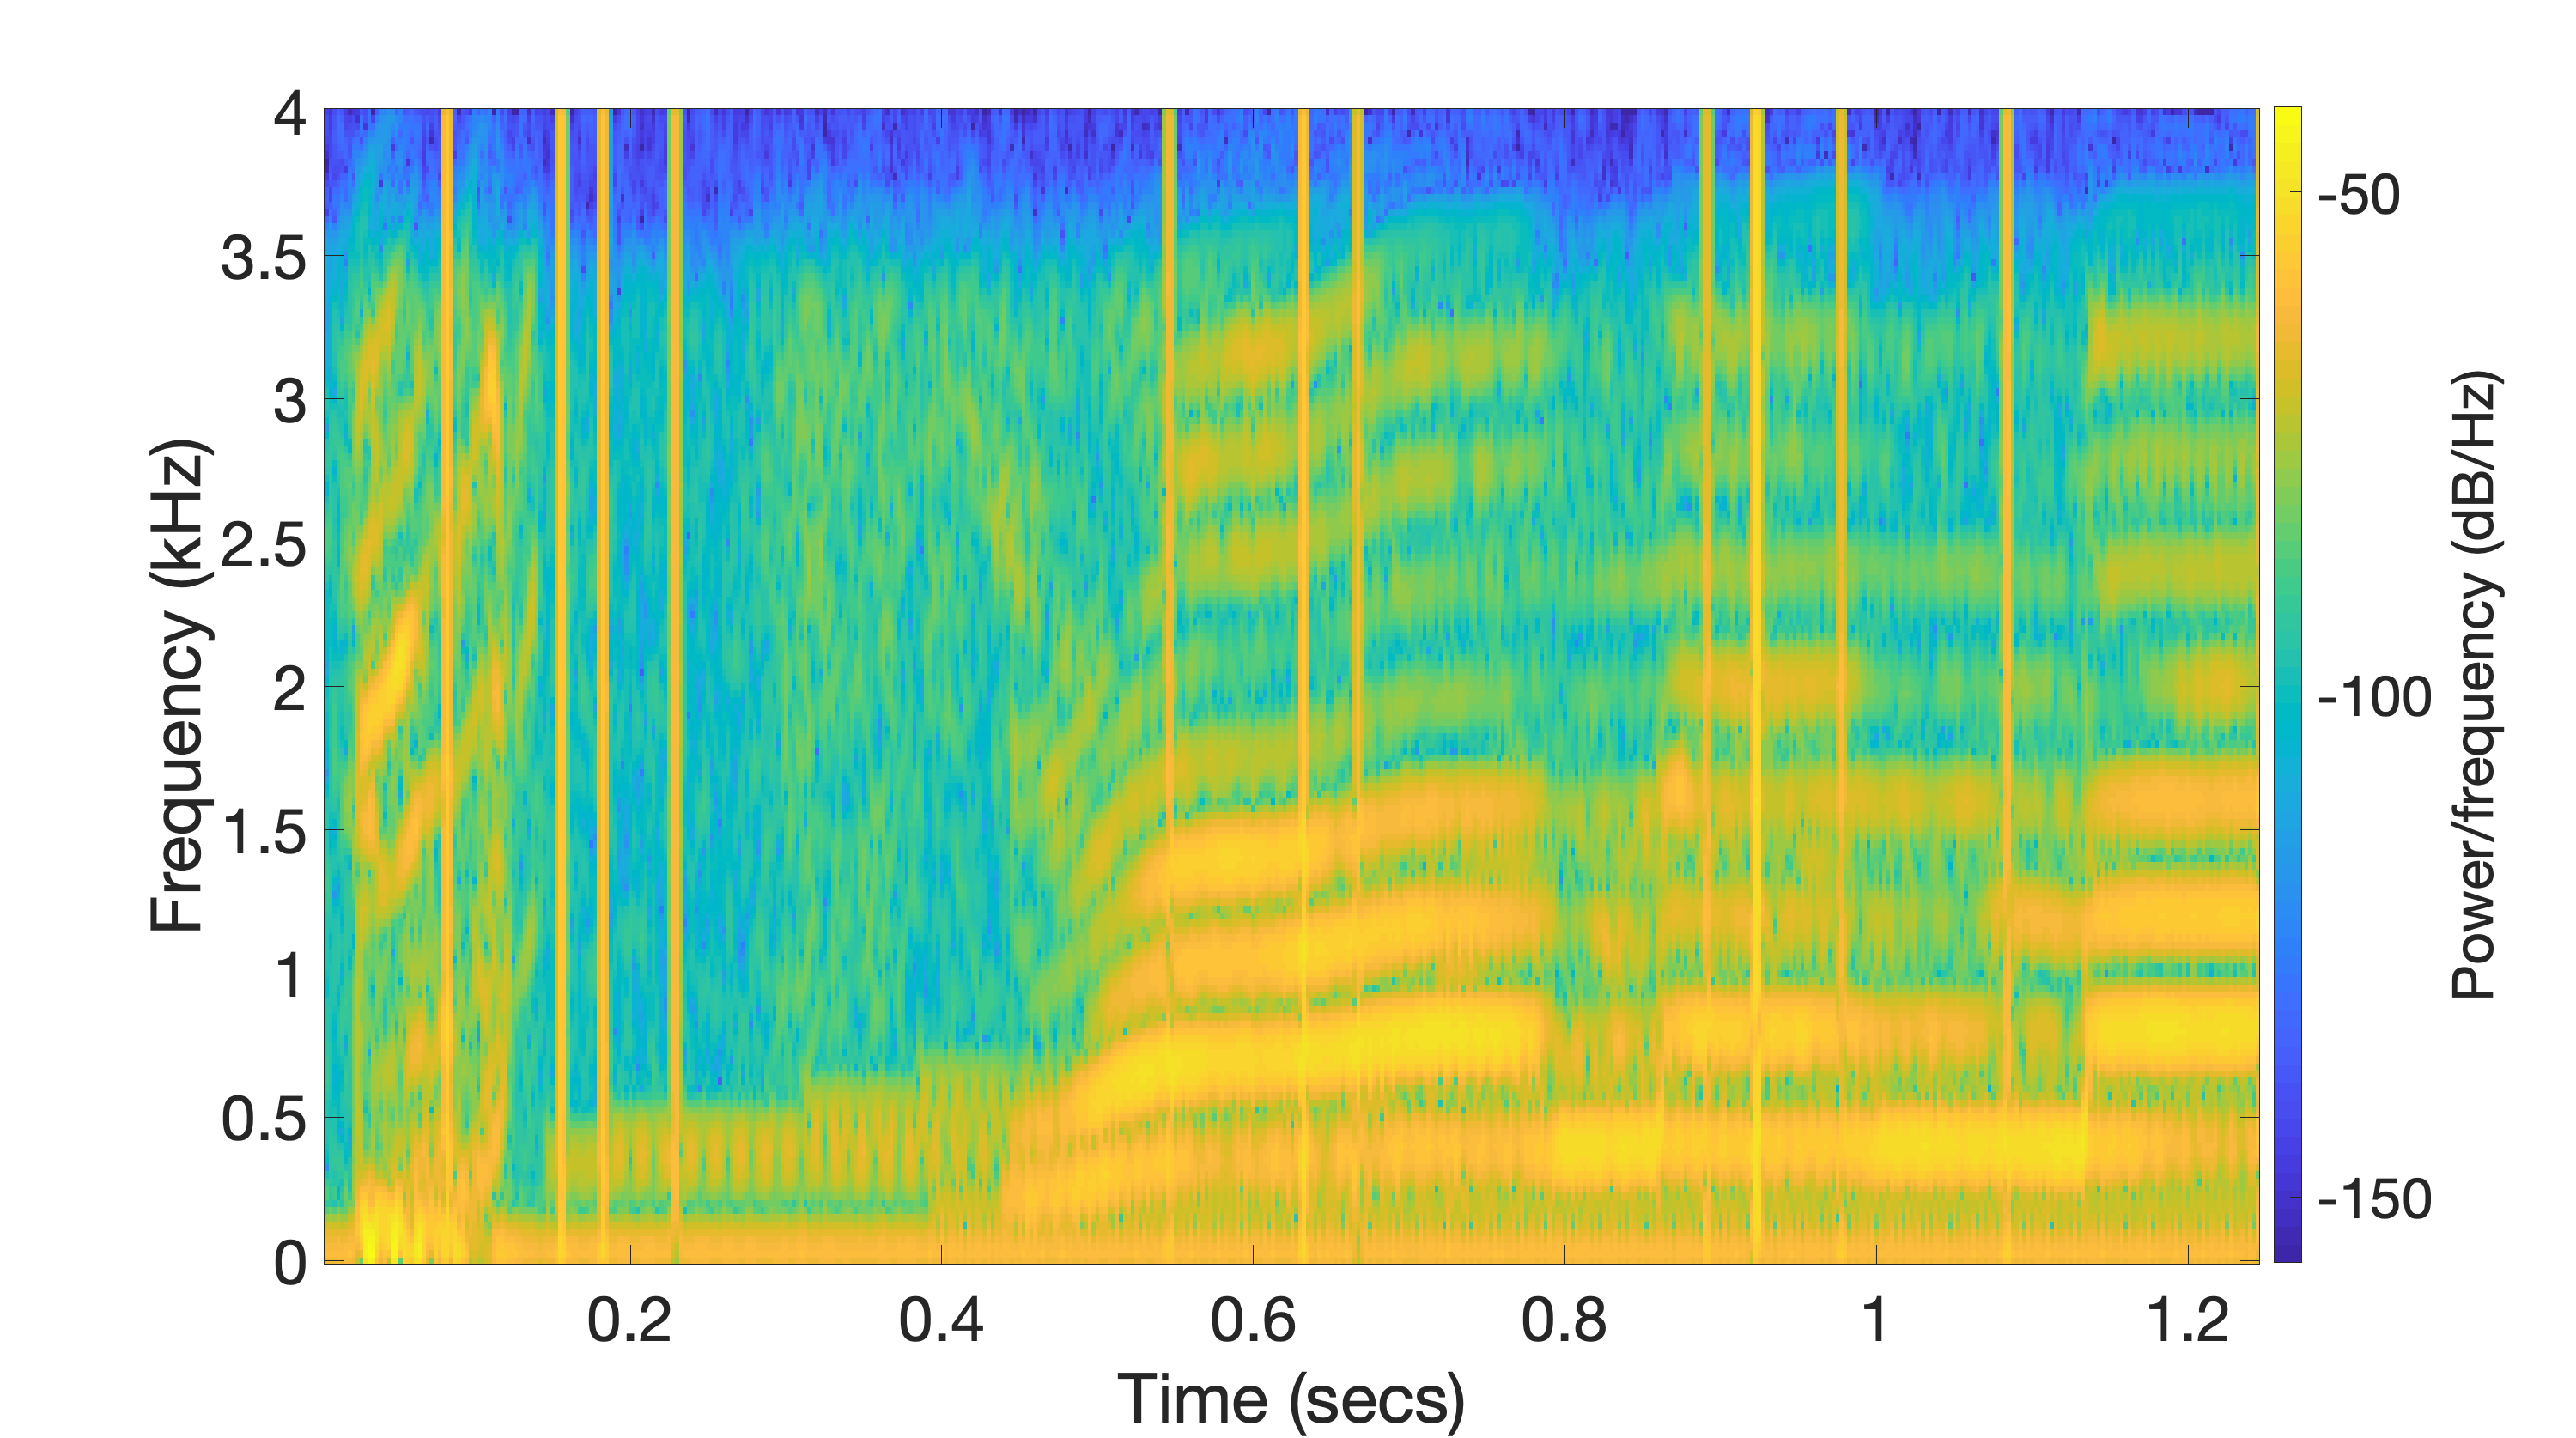
\includegraphics[width= 0.8\textwidth]{figures/R1c_spectrogram.png}
	\caption{Spectrogram.}
	\label{fig:R1c_spectrogram}
\end{figure}
\end{comment}
\begin{figure}[htbp]
	\centering
	\begin{minipage}[b]{.49\textwidth}
		\centering
		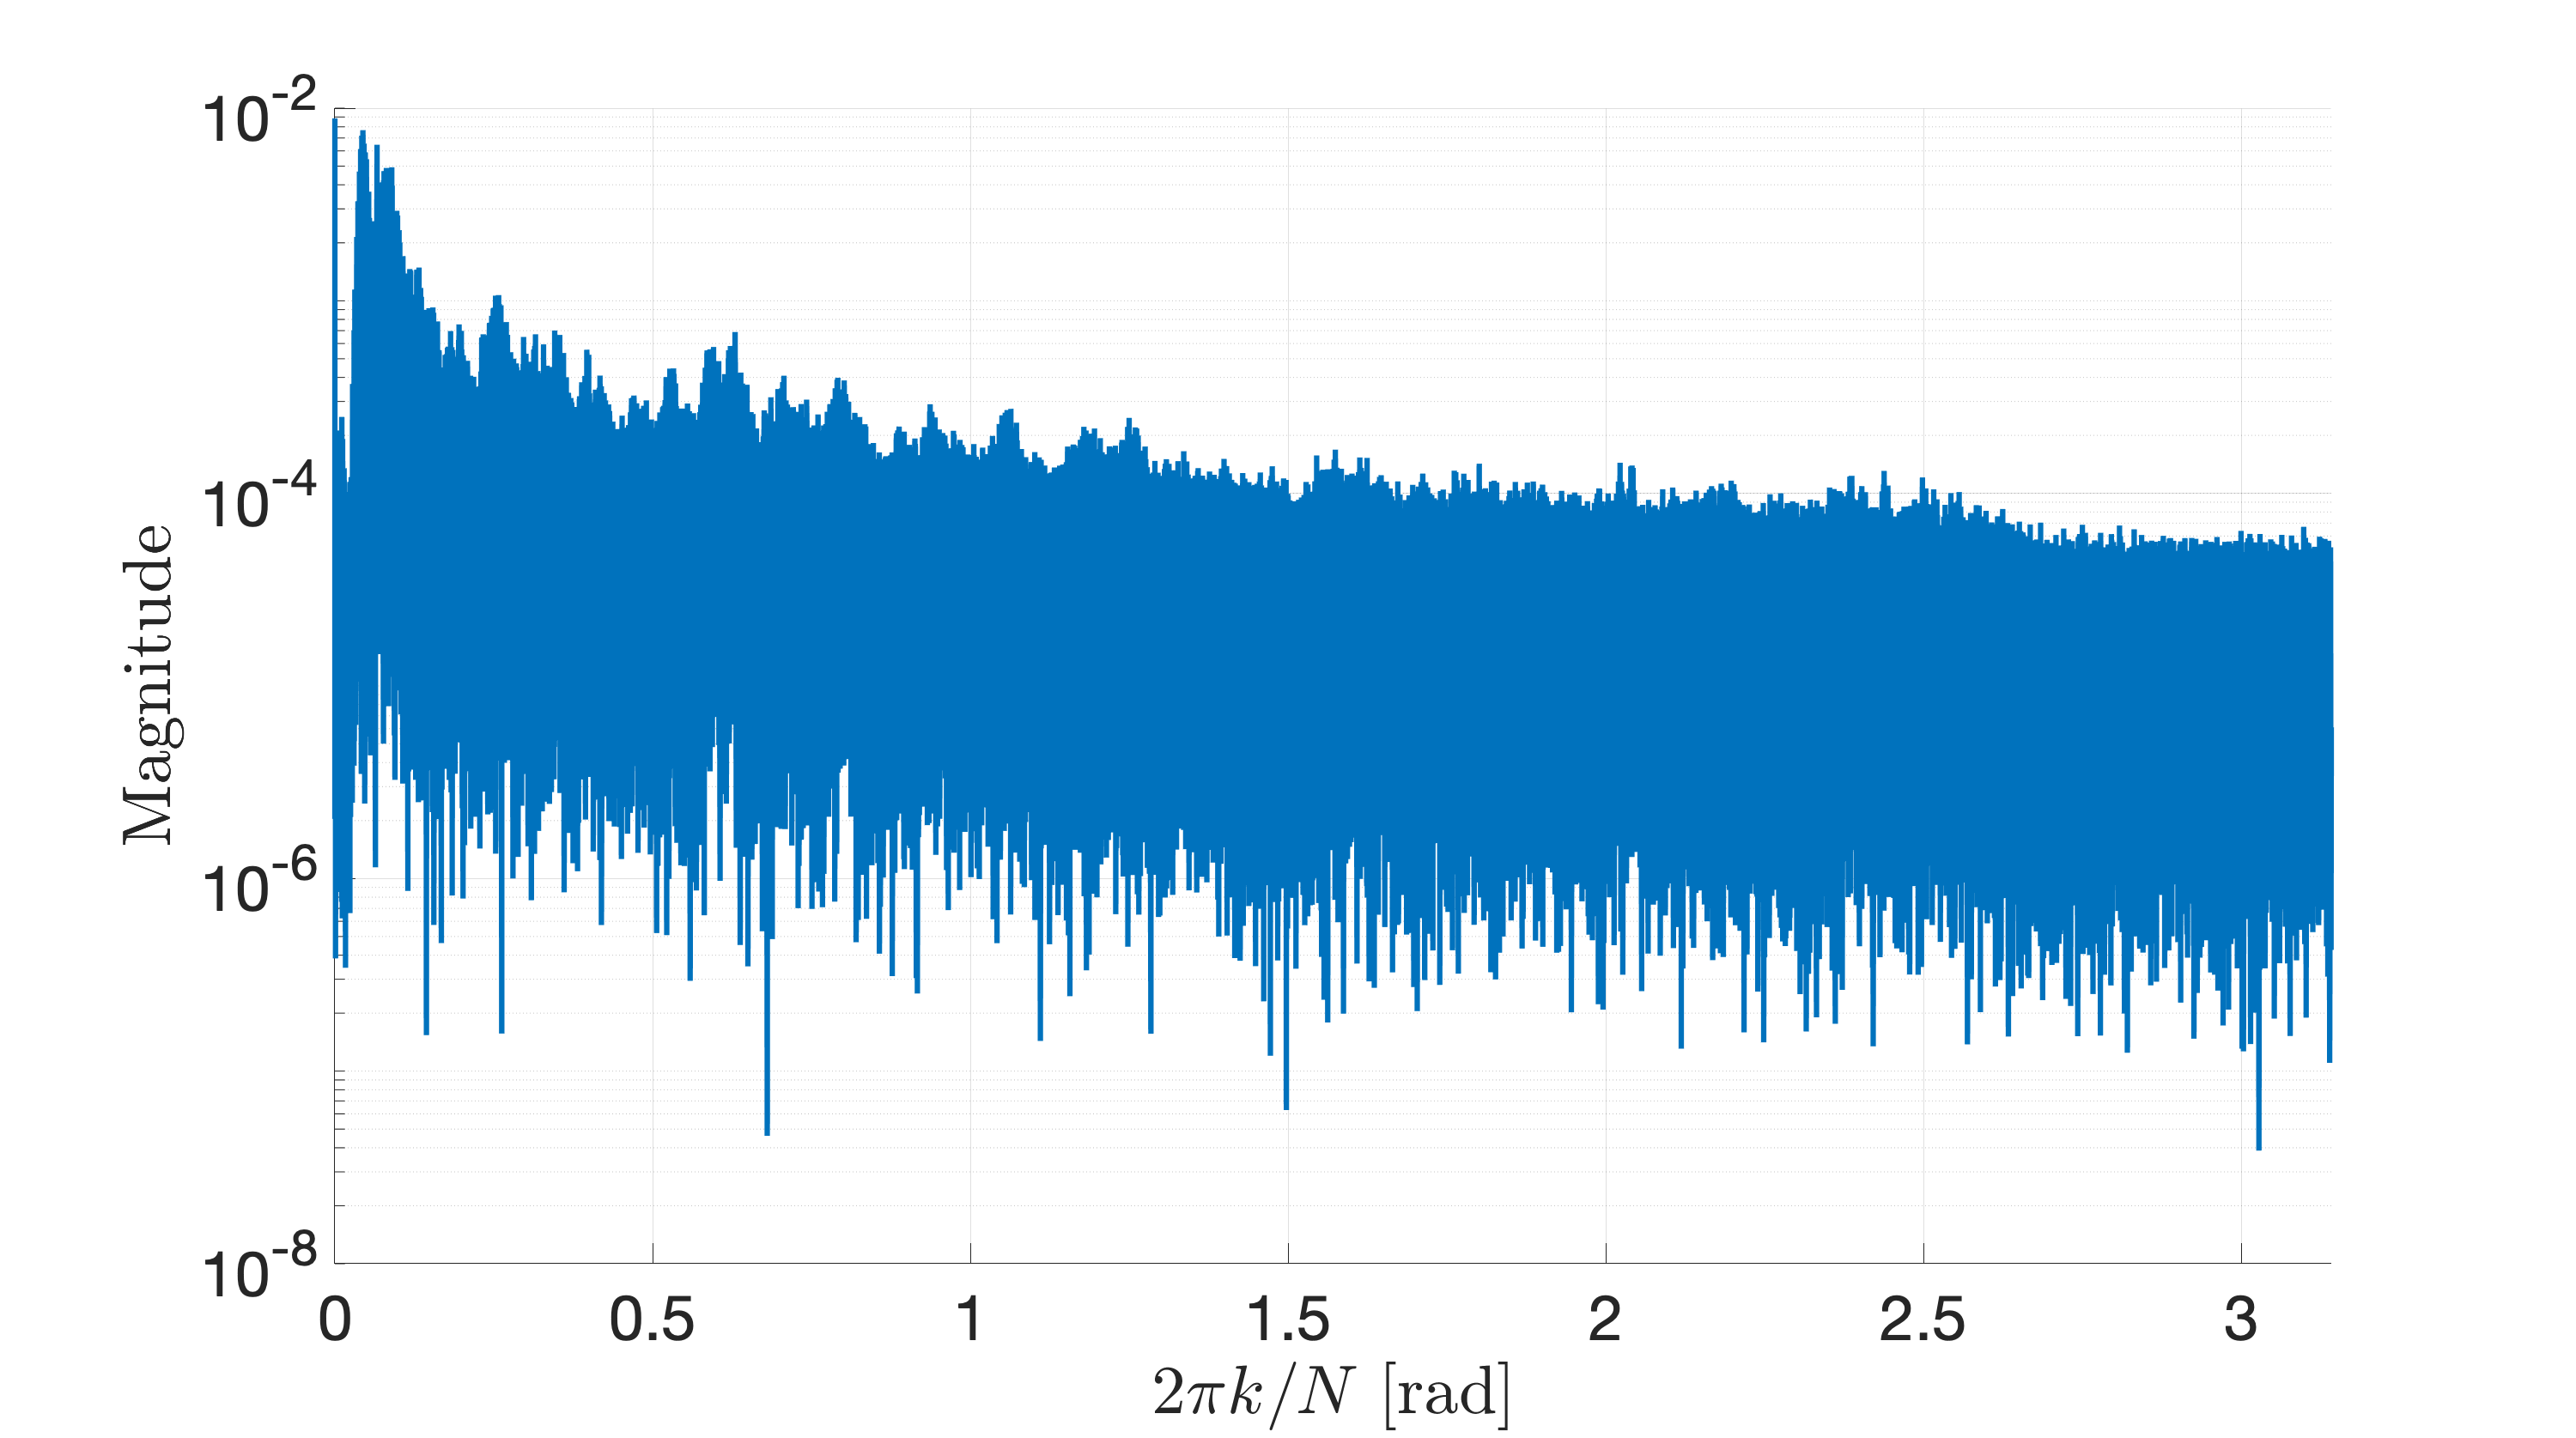
\includegraphics[width= 1.1\textwidth]{figures/R1c.png}
		\caption{Magnitude spectrum of the original sound signal.}
		\label{fig:R1c}
	\end{minipage}
	\hfill
	\begin{minipage}[b]{.49\textwidth}
		\centering
		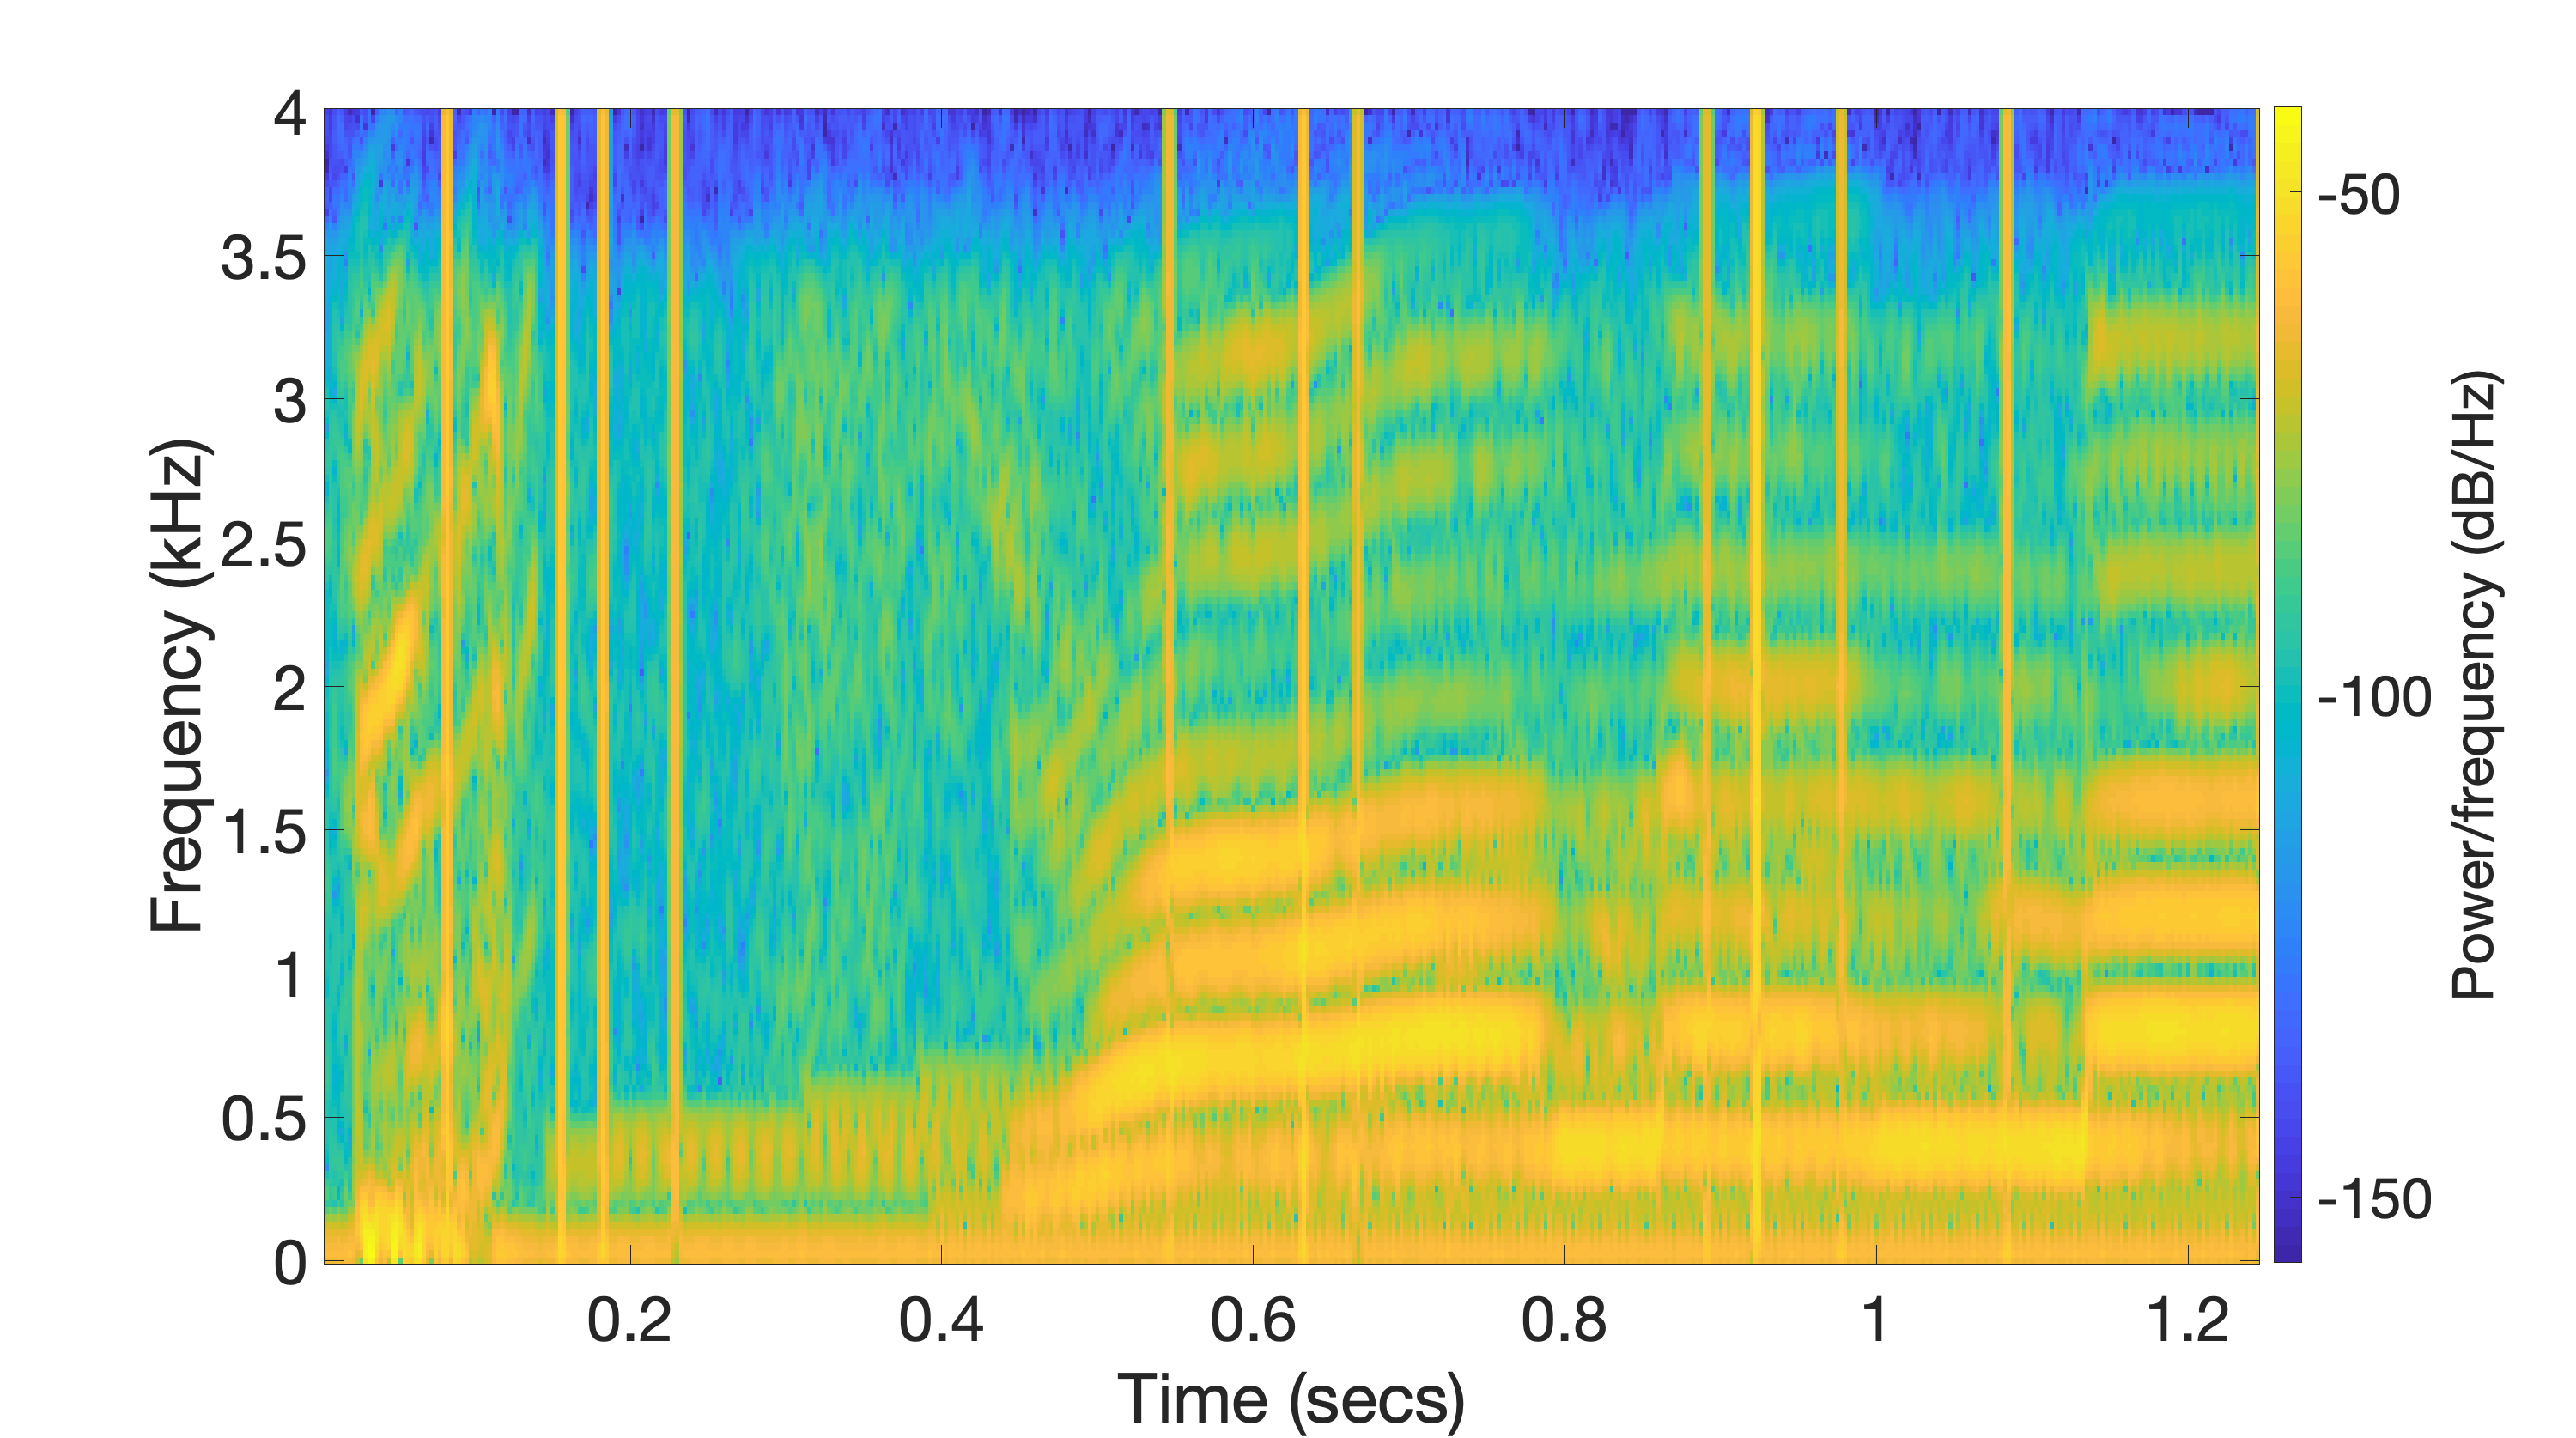
\includegraphics[width= 1.1\textwidth]{figures/R1c_spectrogram.png}
		\caption{Spectrogram.}
		\label{fig:R1c_spectrogram}
	\end{minipage}
\end{figure}

\section{R2. Filtering with an LTI filter}
\subsection{R2.a) Butterworth low-pass filter}
In this and in the following section, two filters are devised to remove the impulsive noise present in the sound signal. First, an LTI Butterworth low-pass filter of order 10 with cutoff frequency $\pi/2$ is computed. The magnitude, in linear coordinates, and phase for this filter are shown in Figs. \ref{fig:R2a_gain} and \ref{fig:R2a_phase}, respectively. As it is evident analyzing the gain of the filter, it operates in frequency. The gain is unitary for low frequency and decreases for high frequencies. That is, it attenuates frequencies to the right of the vertical dashed line, which represents the cutoff frequency, and the frequencies to the left are not affected by the filter in terms of amplitude.

\begin{figure}[htbp]
	\centering
	\begin{minipage}[b]{.49\textwidth}
		\centering
		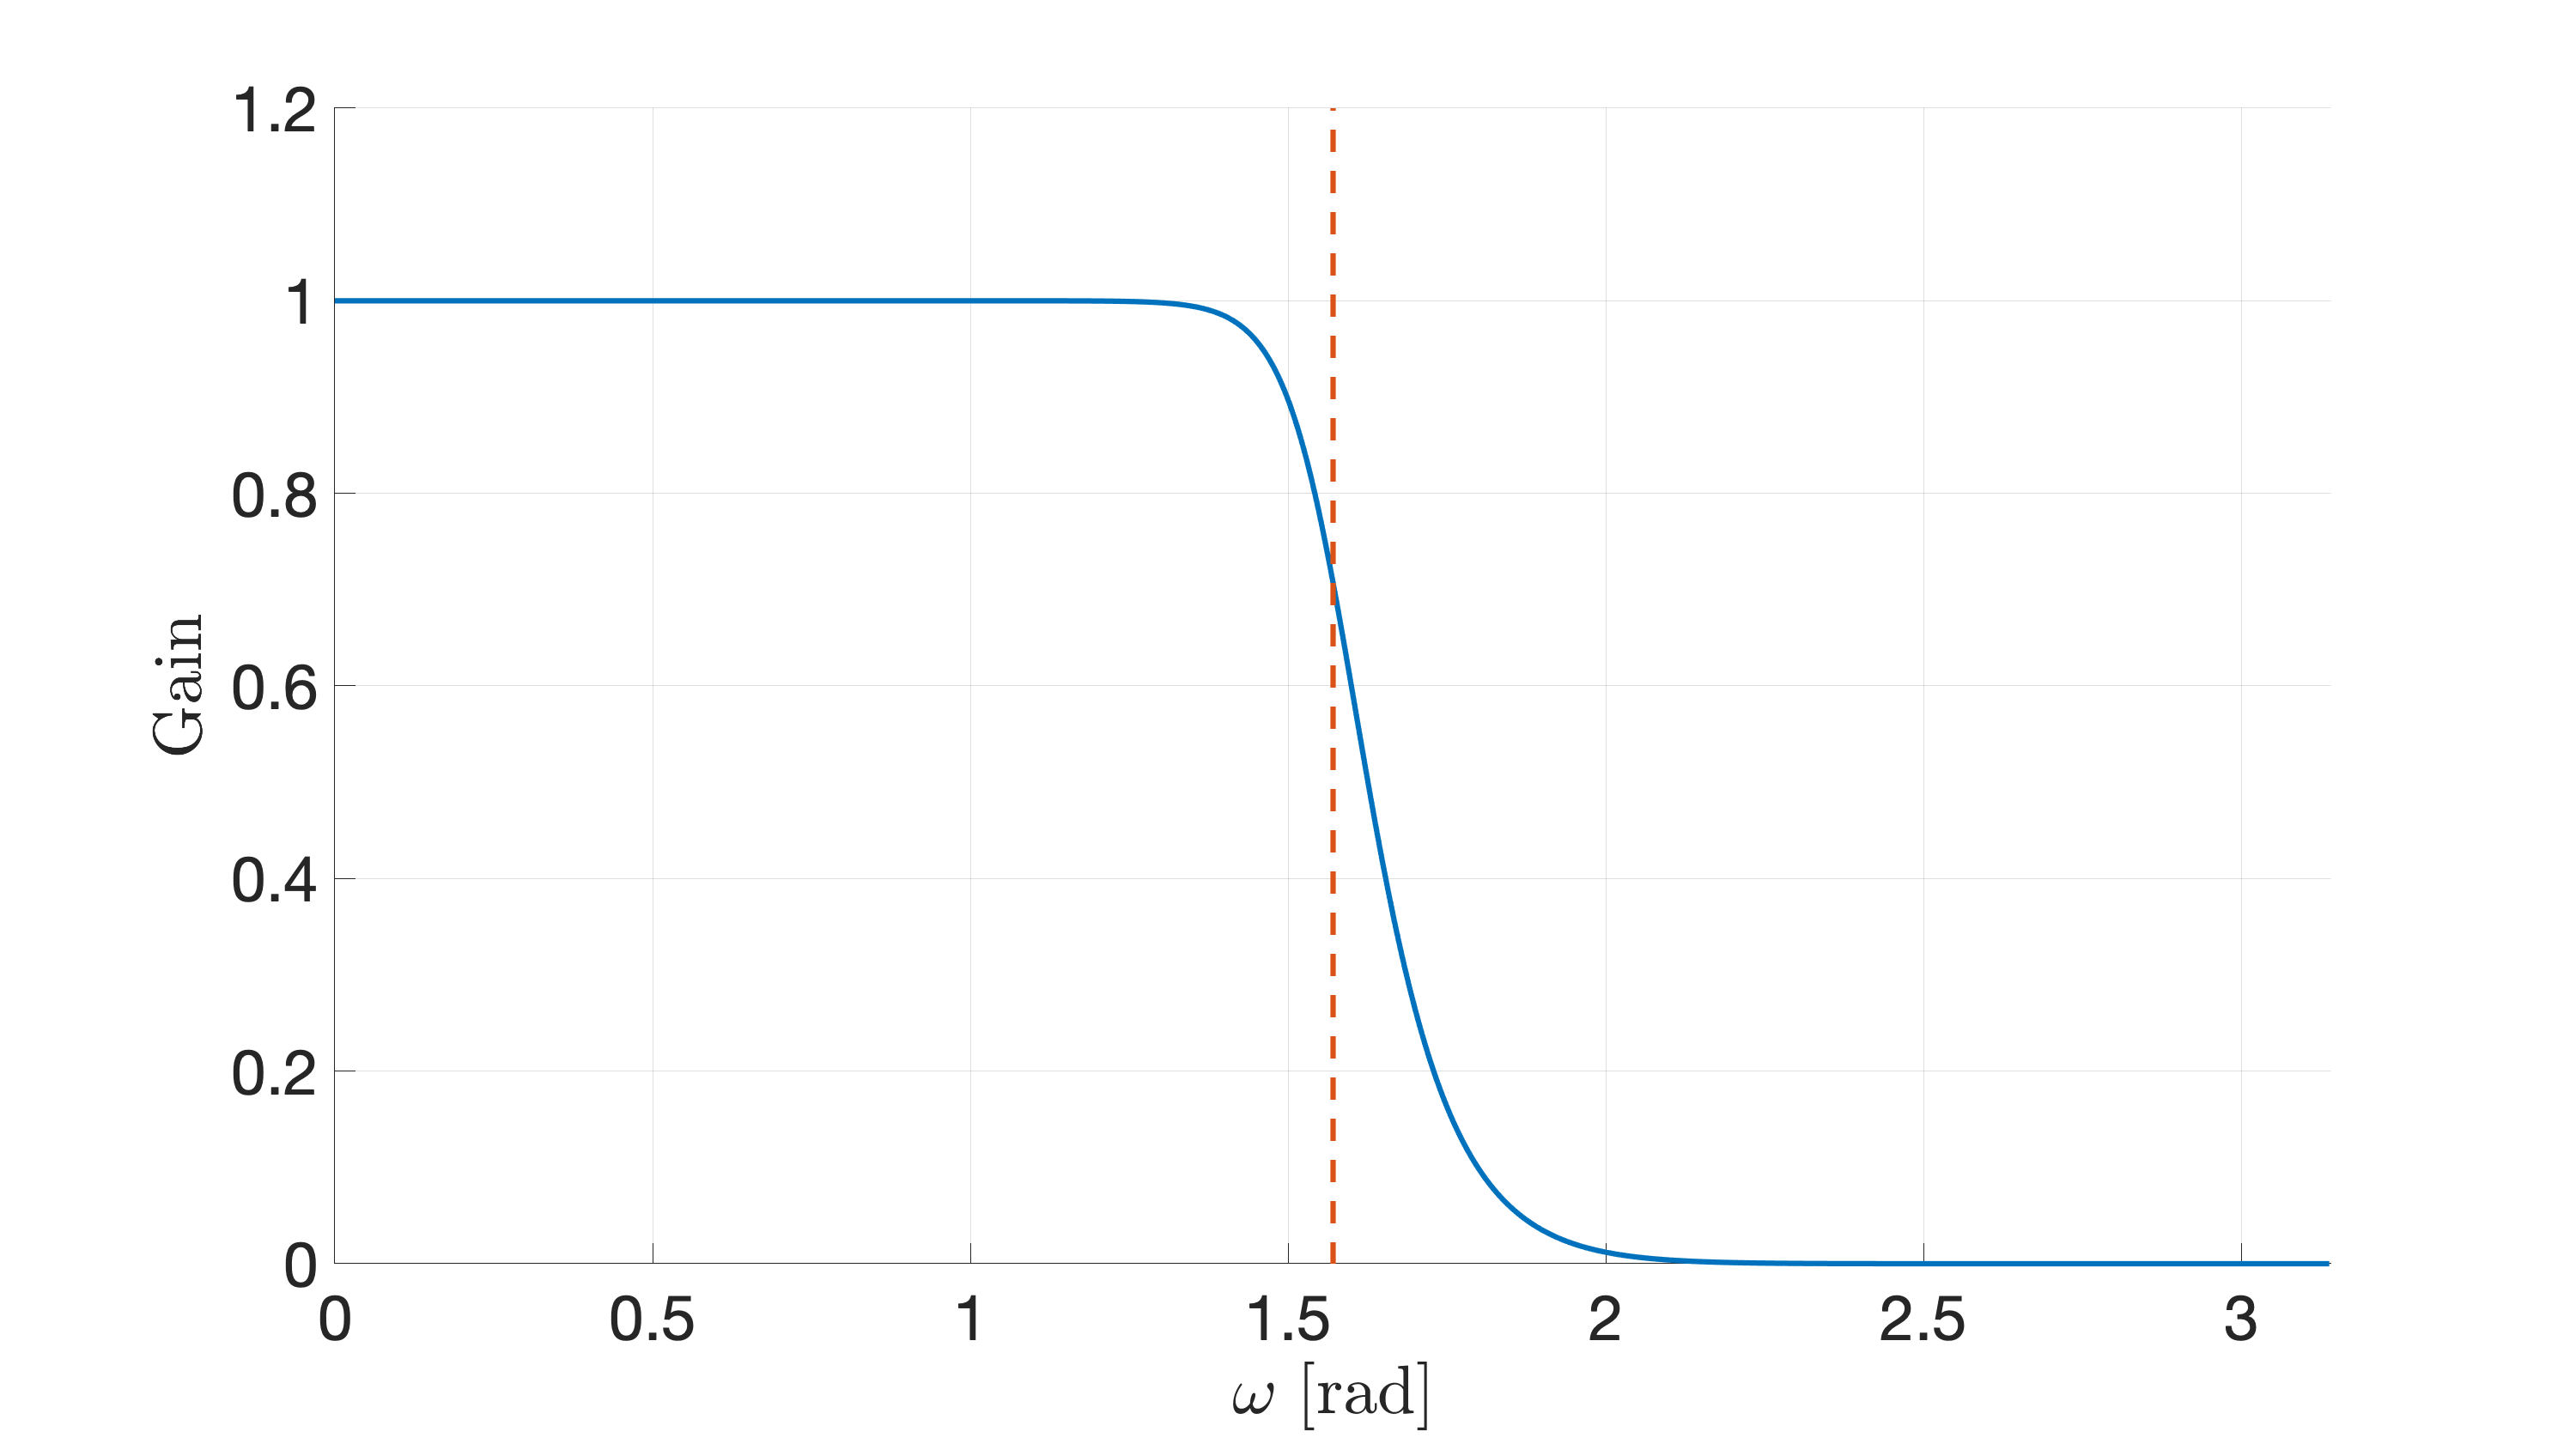
\includegraphics[width= 1.1\textwidth]{figures/R2a_gain.png}
		\caption{Gain in linear coordinates of the LTI filter.}
		\label{fig:R2a_gain}
	\end{minipage}
	\hfill
	\begin{minipage}[b]{.49\textwidth}
		\centering
		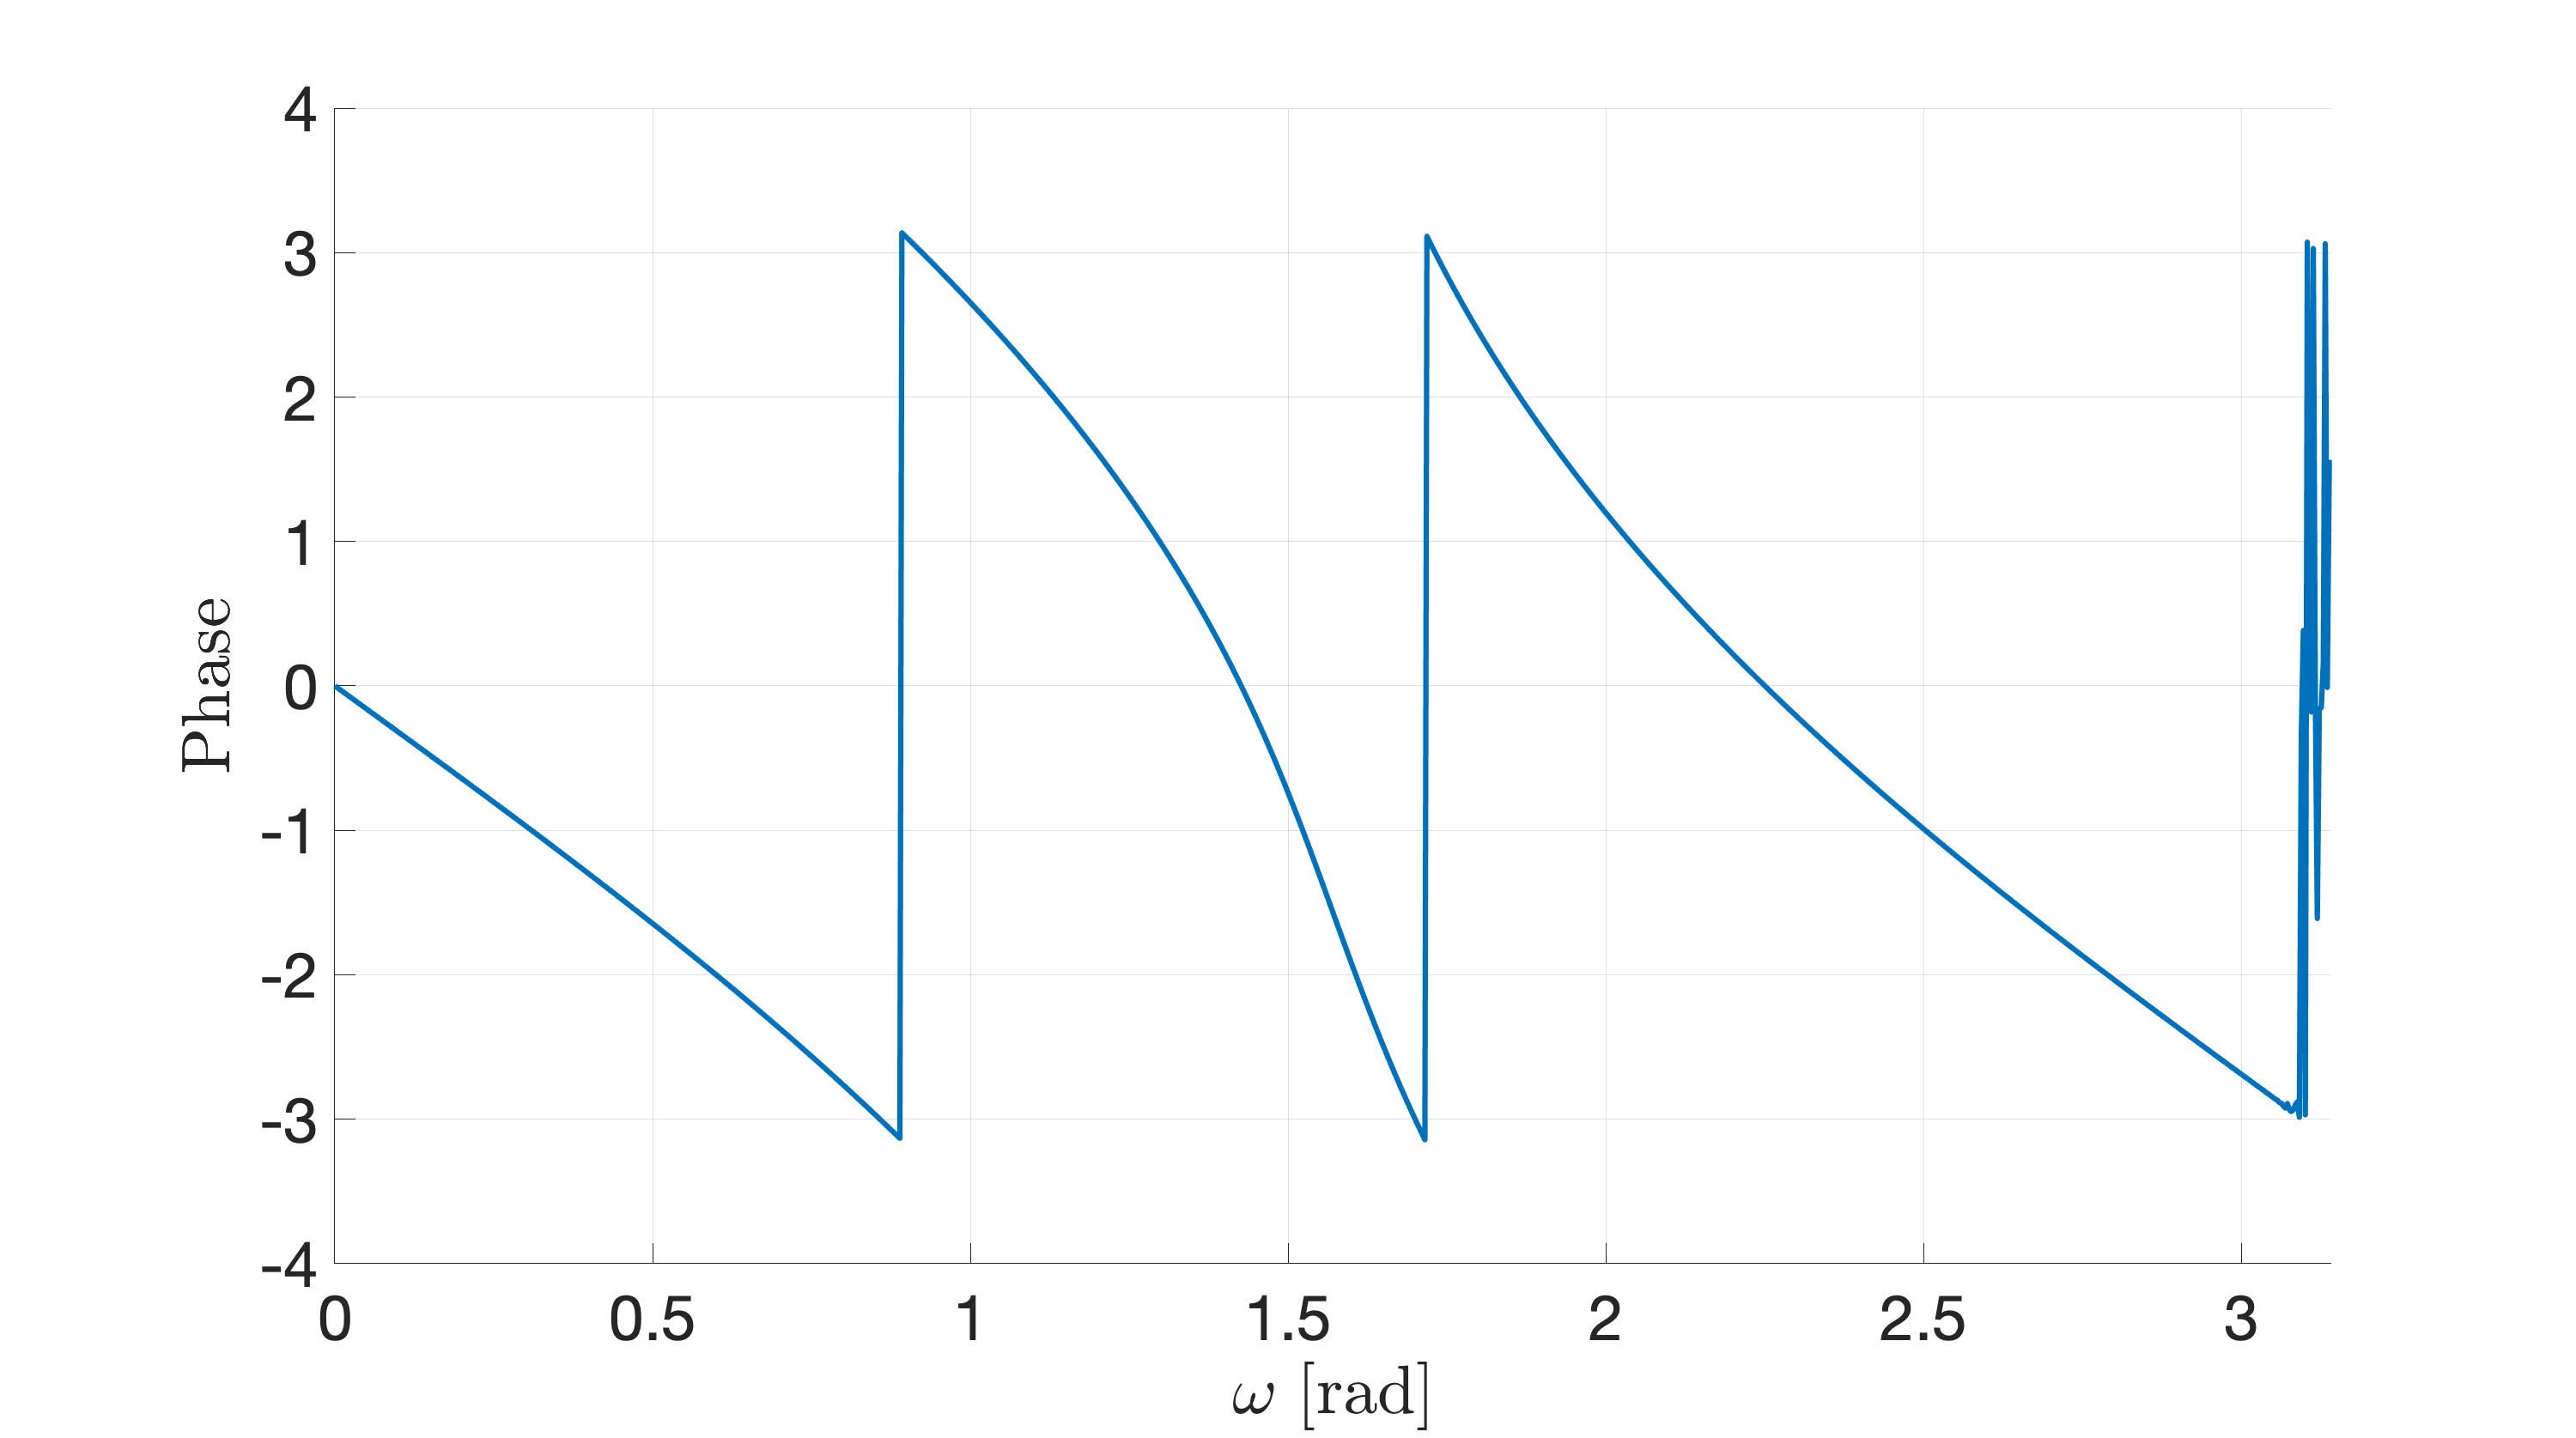
\includegraphics[width= 1.1\textwidth]{figures/R2a_phase.png}
		\caption{Phase of the LTI filter.}
		\label{fig:R2a_phase}
	\end{minipage}
\end{figure}

\subsection{R2.b) Filtered signal}
The continuous time cutoff frequency can be obtained by the following relation
\begin{equation*}
\Omega = \omega/T \iff f_{co} = \frac{\omega}{2\pi}f_s = 2 \text{kHz}\:,
\end{equation*}
where $T$ and $f_s$ are, respectively, the sampling period and the sampling frequency.

\subsection{R2.c) Analysis of the filtered signal in the time domain}

Figs. \ref{fig:R2c}--\ref{fig:R2c_zoomNormal} show the comparison of the filtered signal and the original signal in the time domain for various segments of the song. First, it is seen in Fig. \ref{fig:R2c} that although the noise impulses are attenuated in relation to the original signal, they are still very significant. This is expected, since in the frequency domain the impulses are represented by a constant and this filter is attenuating only the portion that is in the higher frequencies. Although the segments of the signal which are not corrupted by noise are attenuated, this attenuation is not significant. Second, Fig. \ref{fig:R2c} shown a zoom of the signal, where it is possible to see the effect of the distortion caused by the filter. Third, in Fig. \ref{fig:R2c_zoomNoise} it is possible to analyze more closely the behavior of the filter after a noise impulse in the time domain. After the noise impulse, as expected, the response of the noiseless signal is superimposed with the impulse response of the filter, which is IIR. The impulse response of the filter is oscillatory and similar to the response of a under-damped second order system. Fourth, in Fig. \ref{fig:R2c_zoomNormal} it is possible to notice the delay introduced by the filter. Furthermore, given that the phase of the filter, represented in \ref{fig:R2a_phase}, is not linear, then the delay of the filter varies with frequency, which is also a source of distortion.

\begin{figure}[htbp]
	\centering
	\begin{minipage}[b]{.49\textwidth}
		\centering
		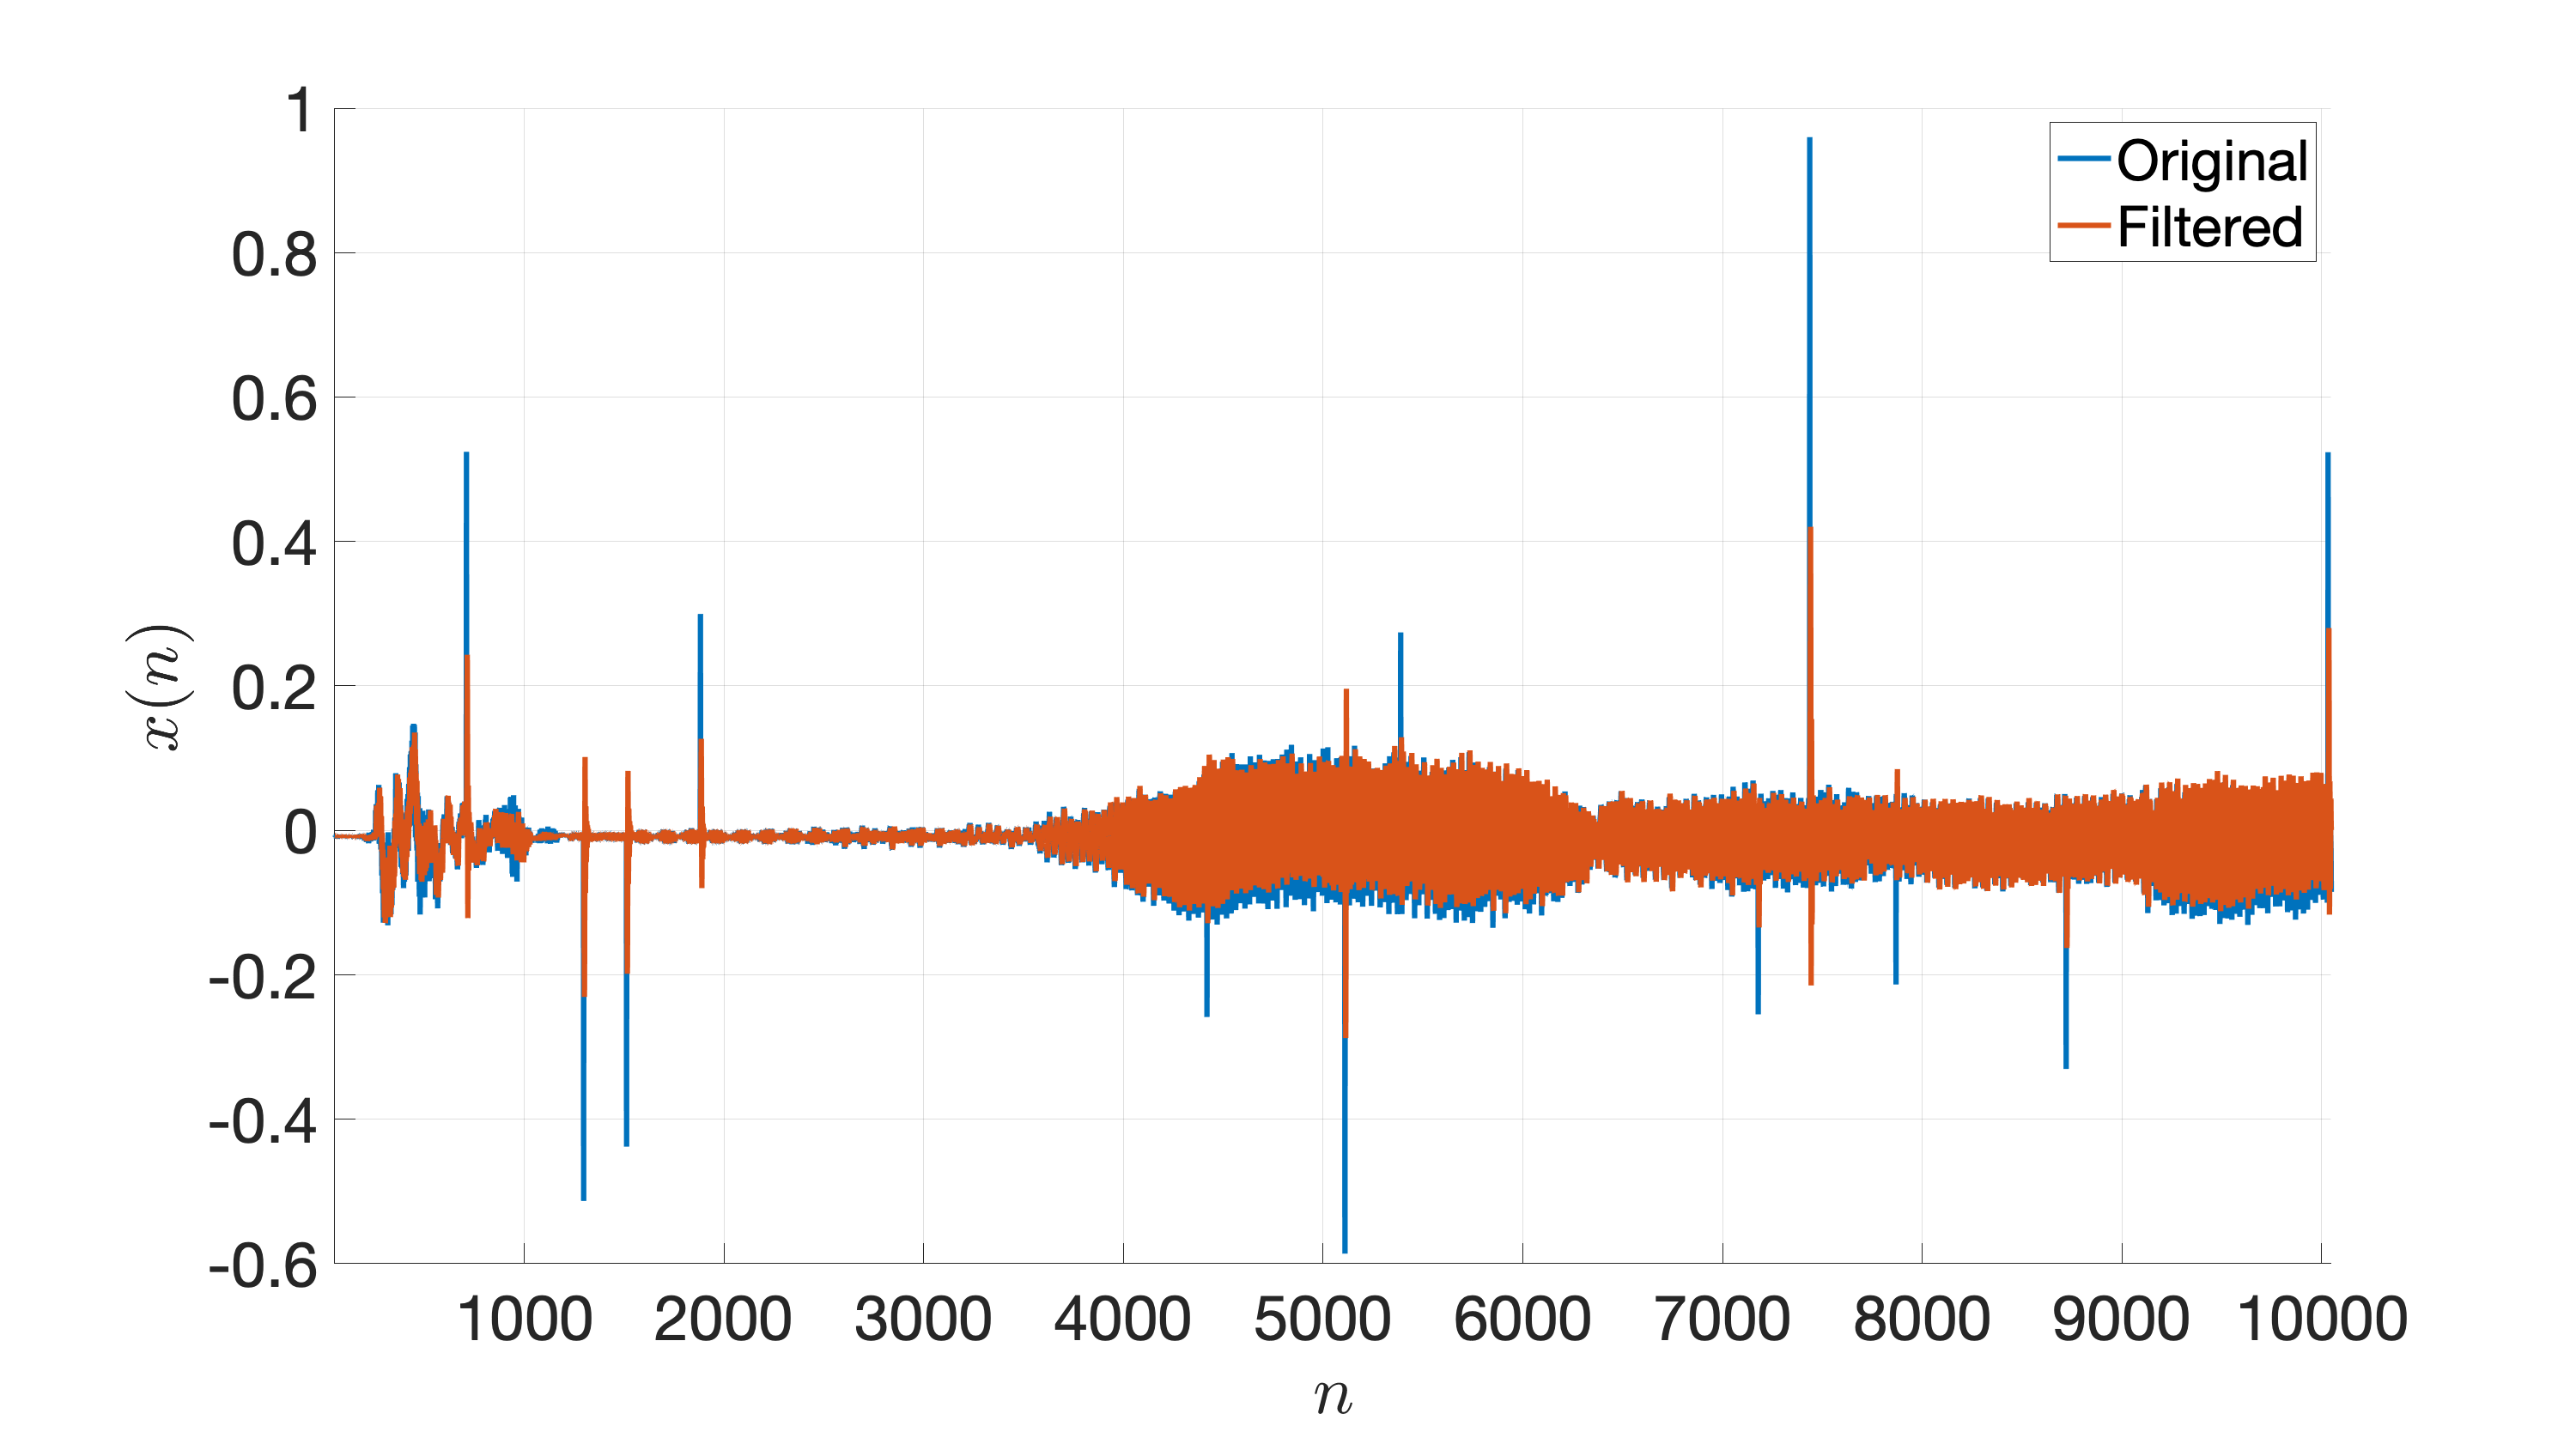
\includegraphics[width= 1.1\textwidth]{figures/R2c.png}
		\caption{Filtered signal.}
		\label{fig:R2c}
	\end{minipage}
	\hfill
	\begin{minipage}[b]{.49\textwidth}
		\centering
		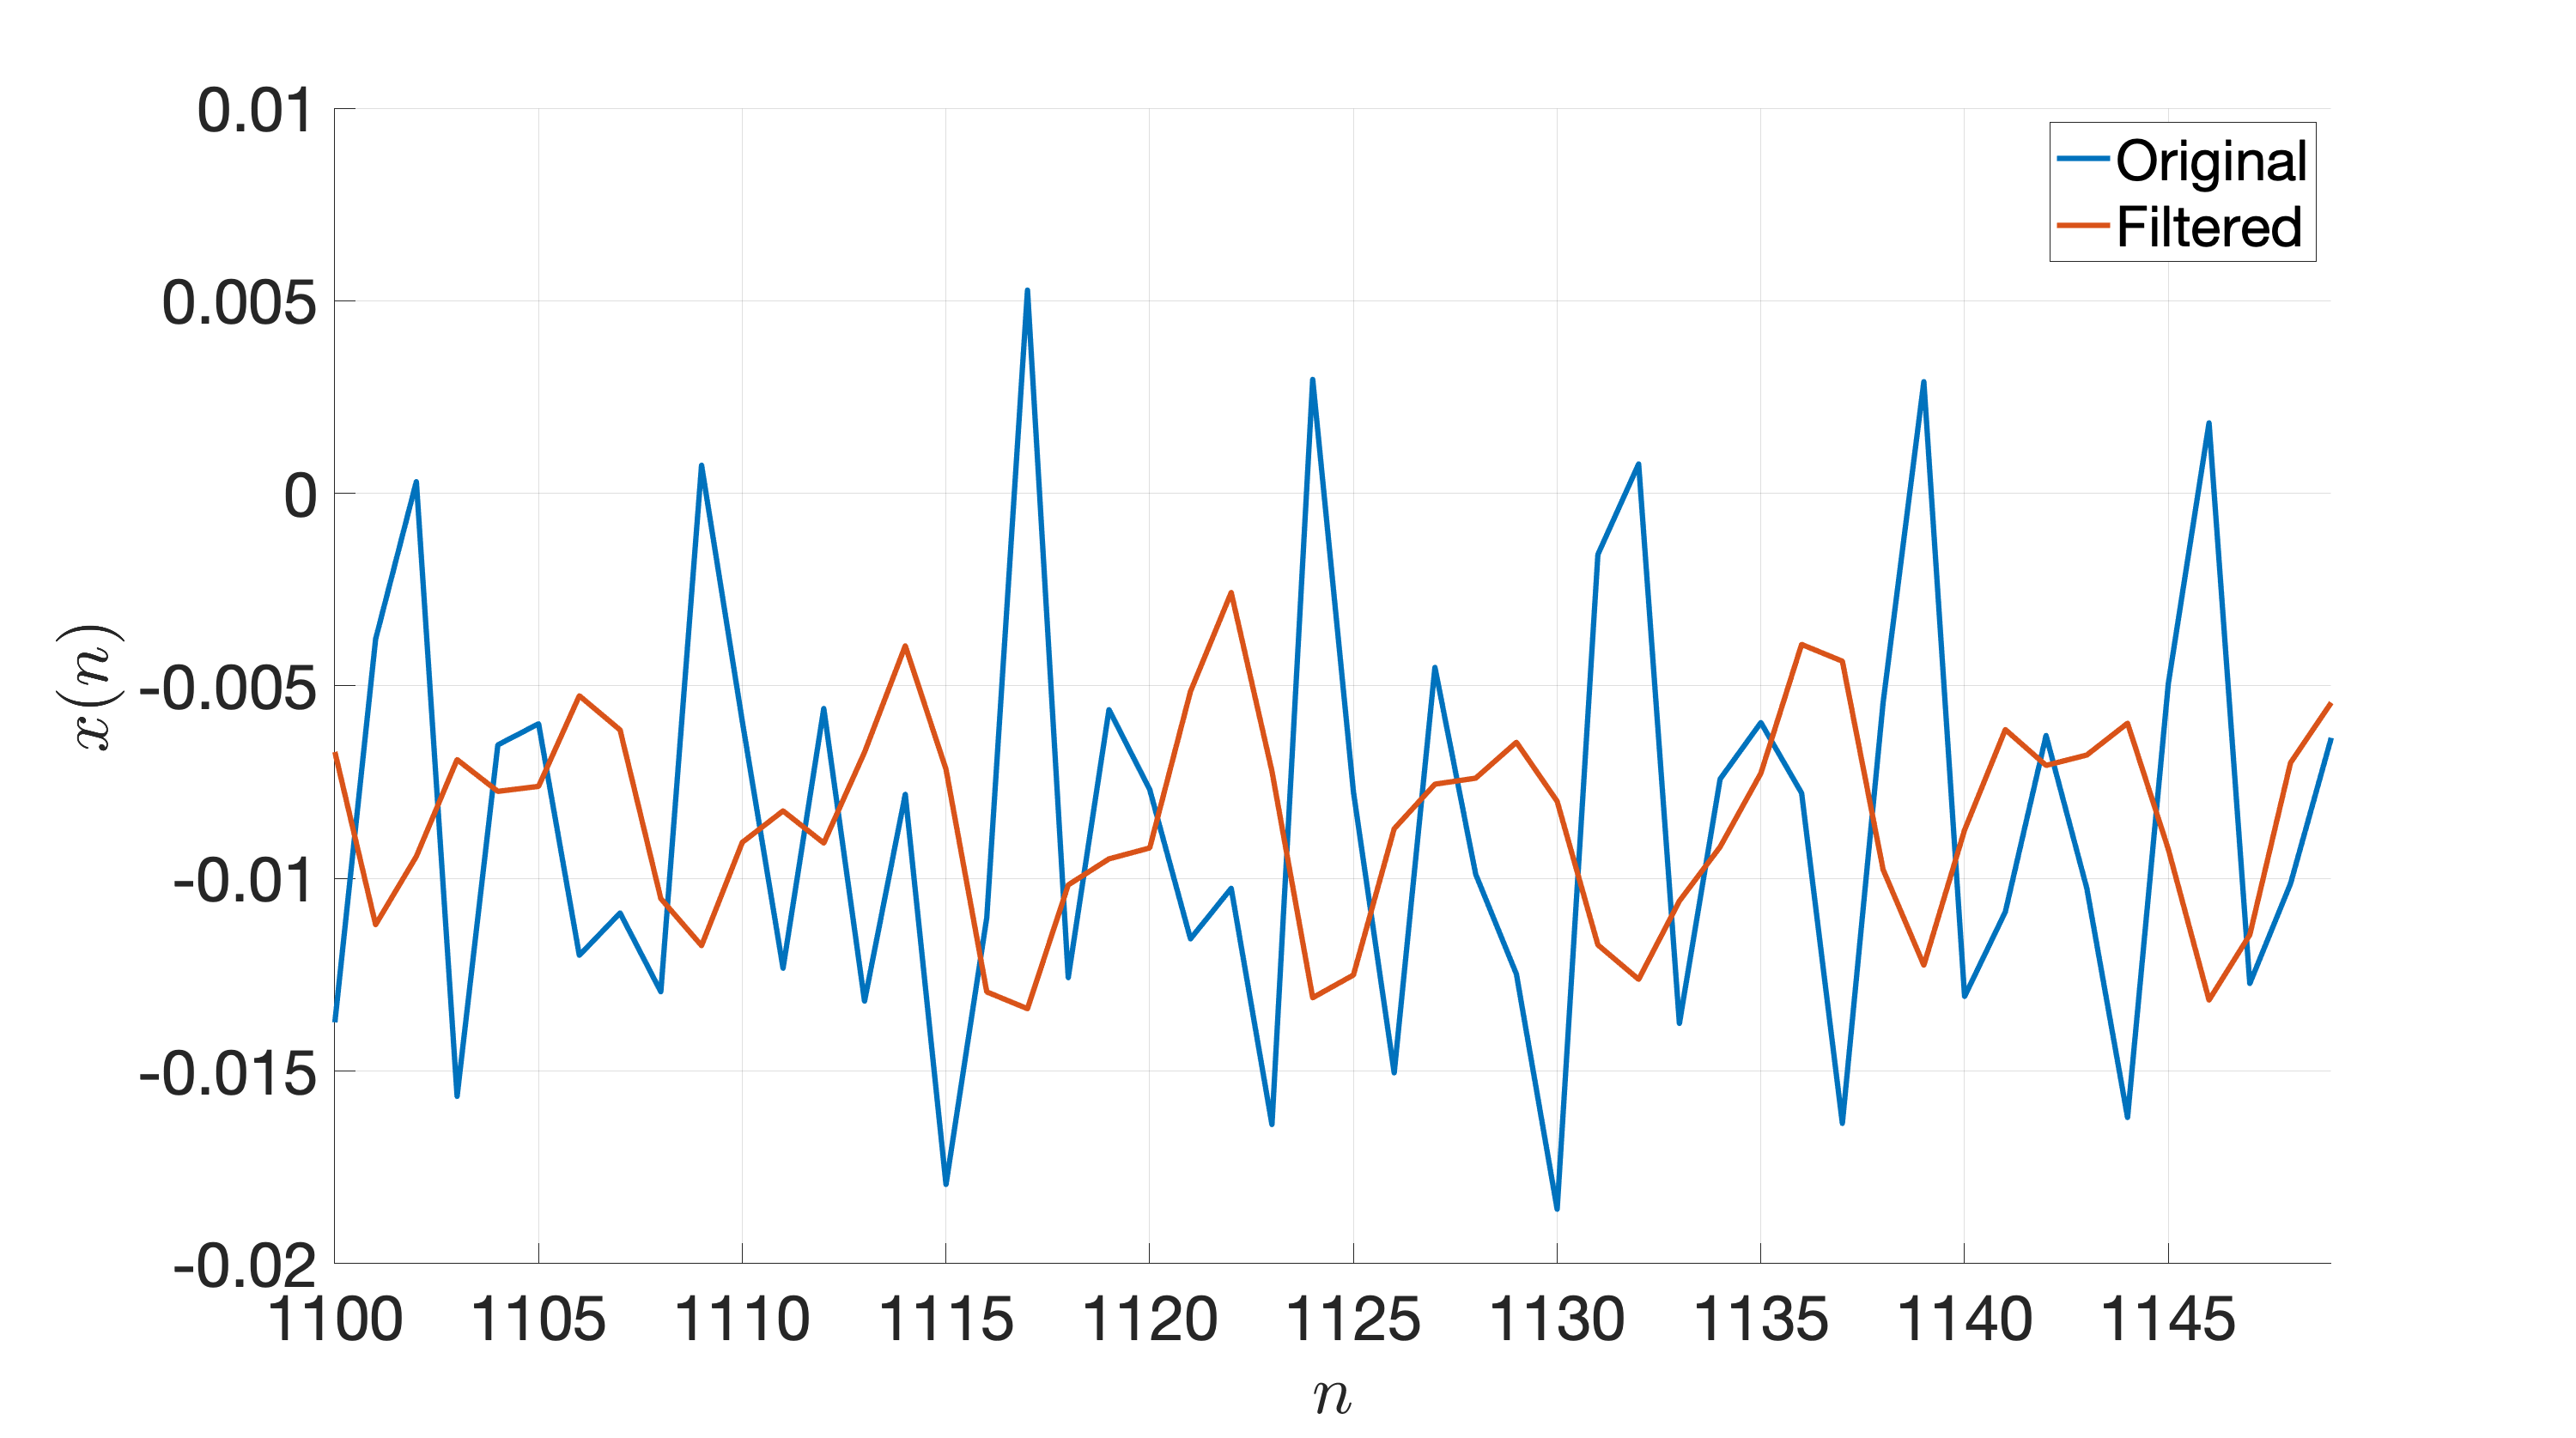
\includegraphics[width= 1.1\textwidth]{figures/R2c_smallAmp.png}
		\caption{Filtered signal.}
		\label{fig:R2c_smallAmp}
	\end{minipage}
\begin{minipage}[b]{.49\textwidth}
	\centering
	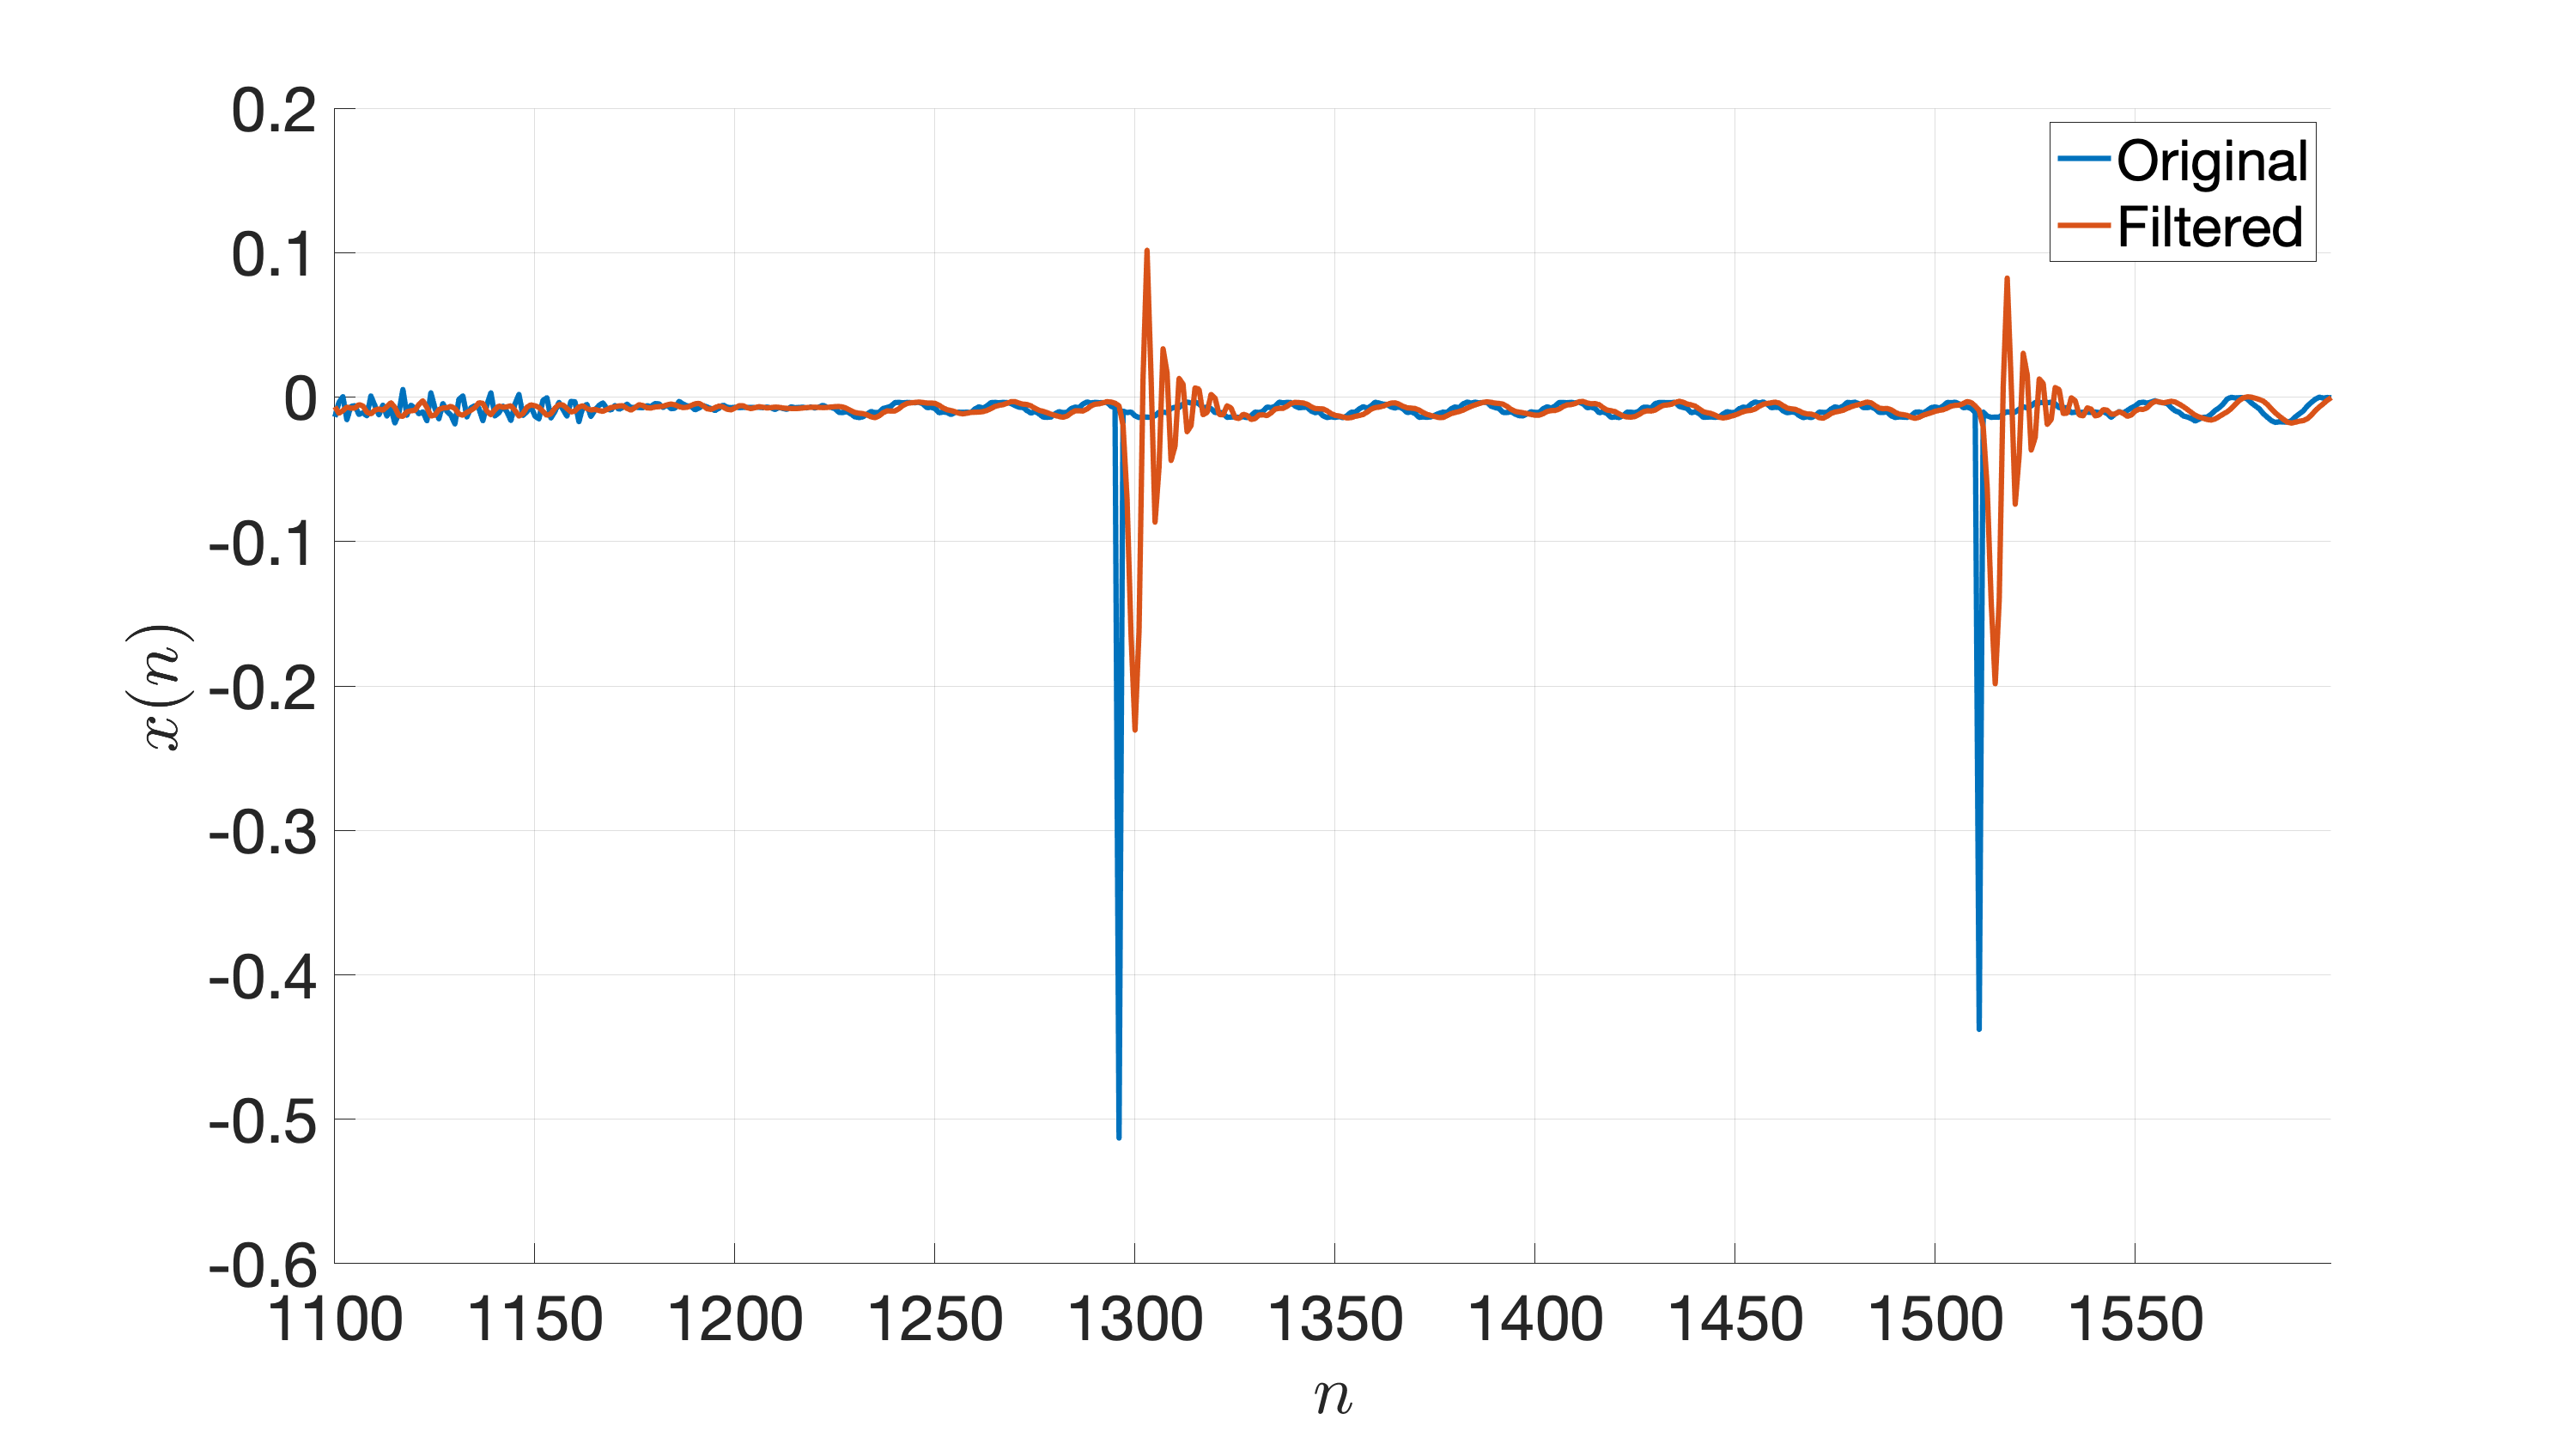
\includegraphics[width= 1.1\textwidth]{figures/R2c_zoomNoise.png}
	\caption{Filtered signal.}
	\label{fig:R2c_zoomNoise}
\end{minipage}
\hfill
\begin{minipage}[b]{.49\textwidth}
	\centering
	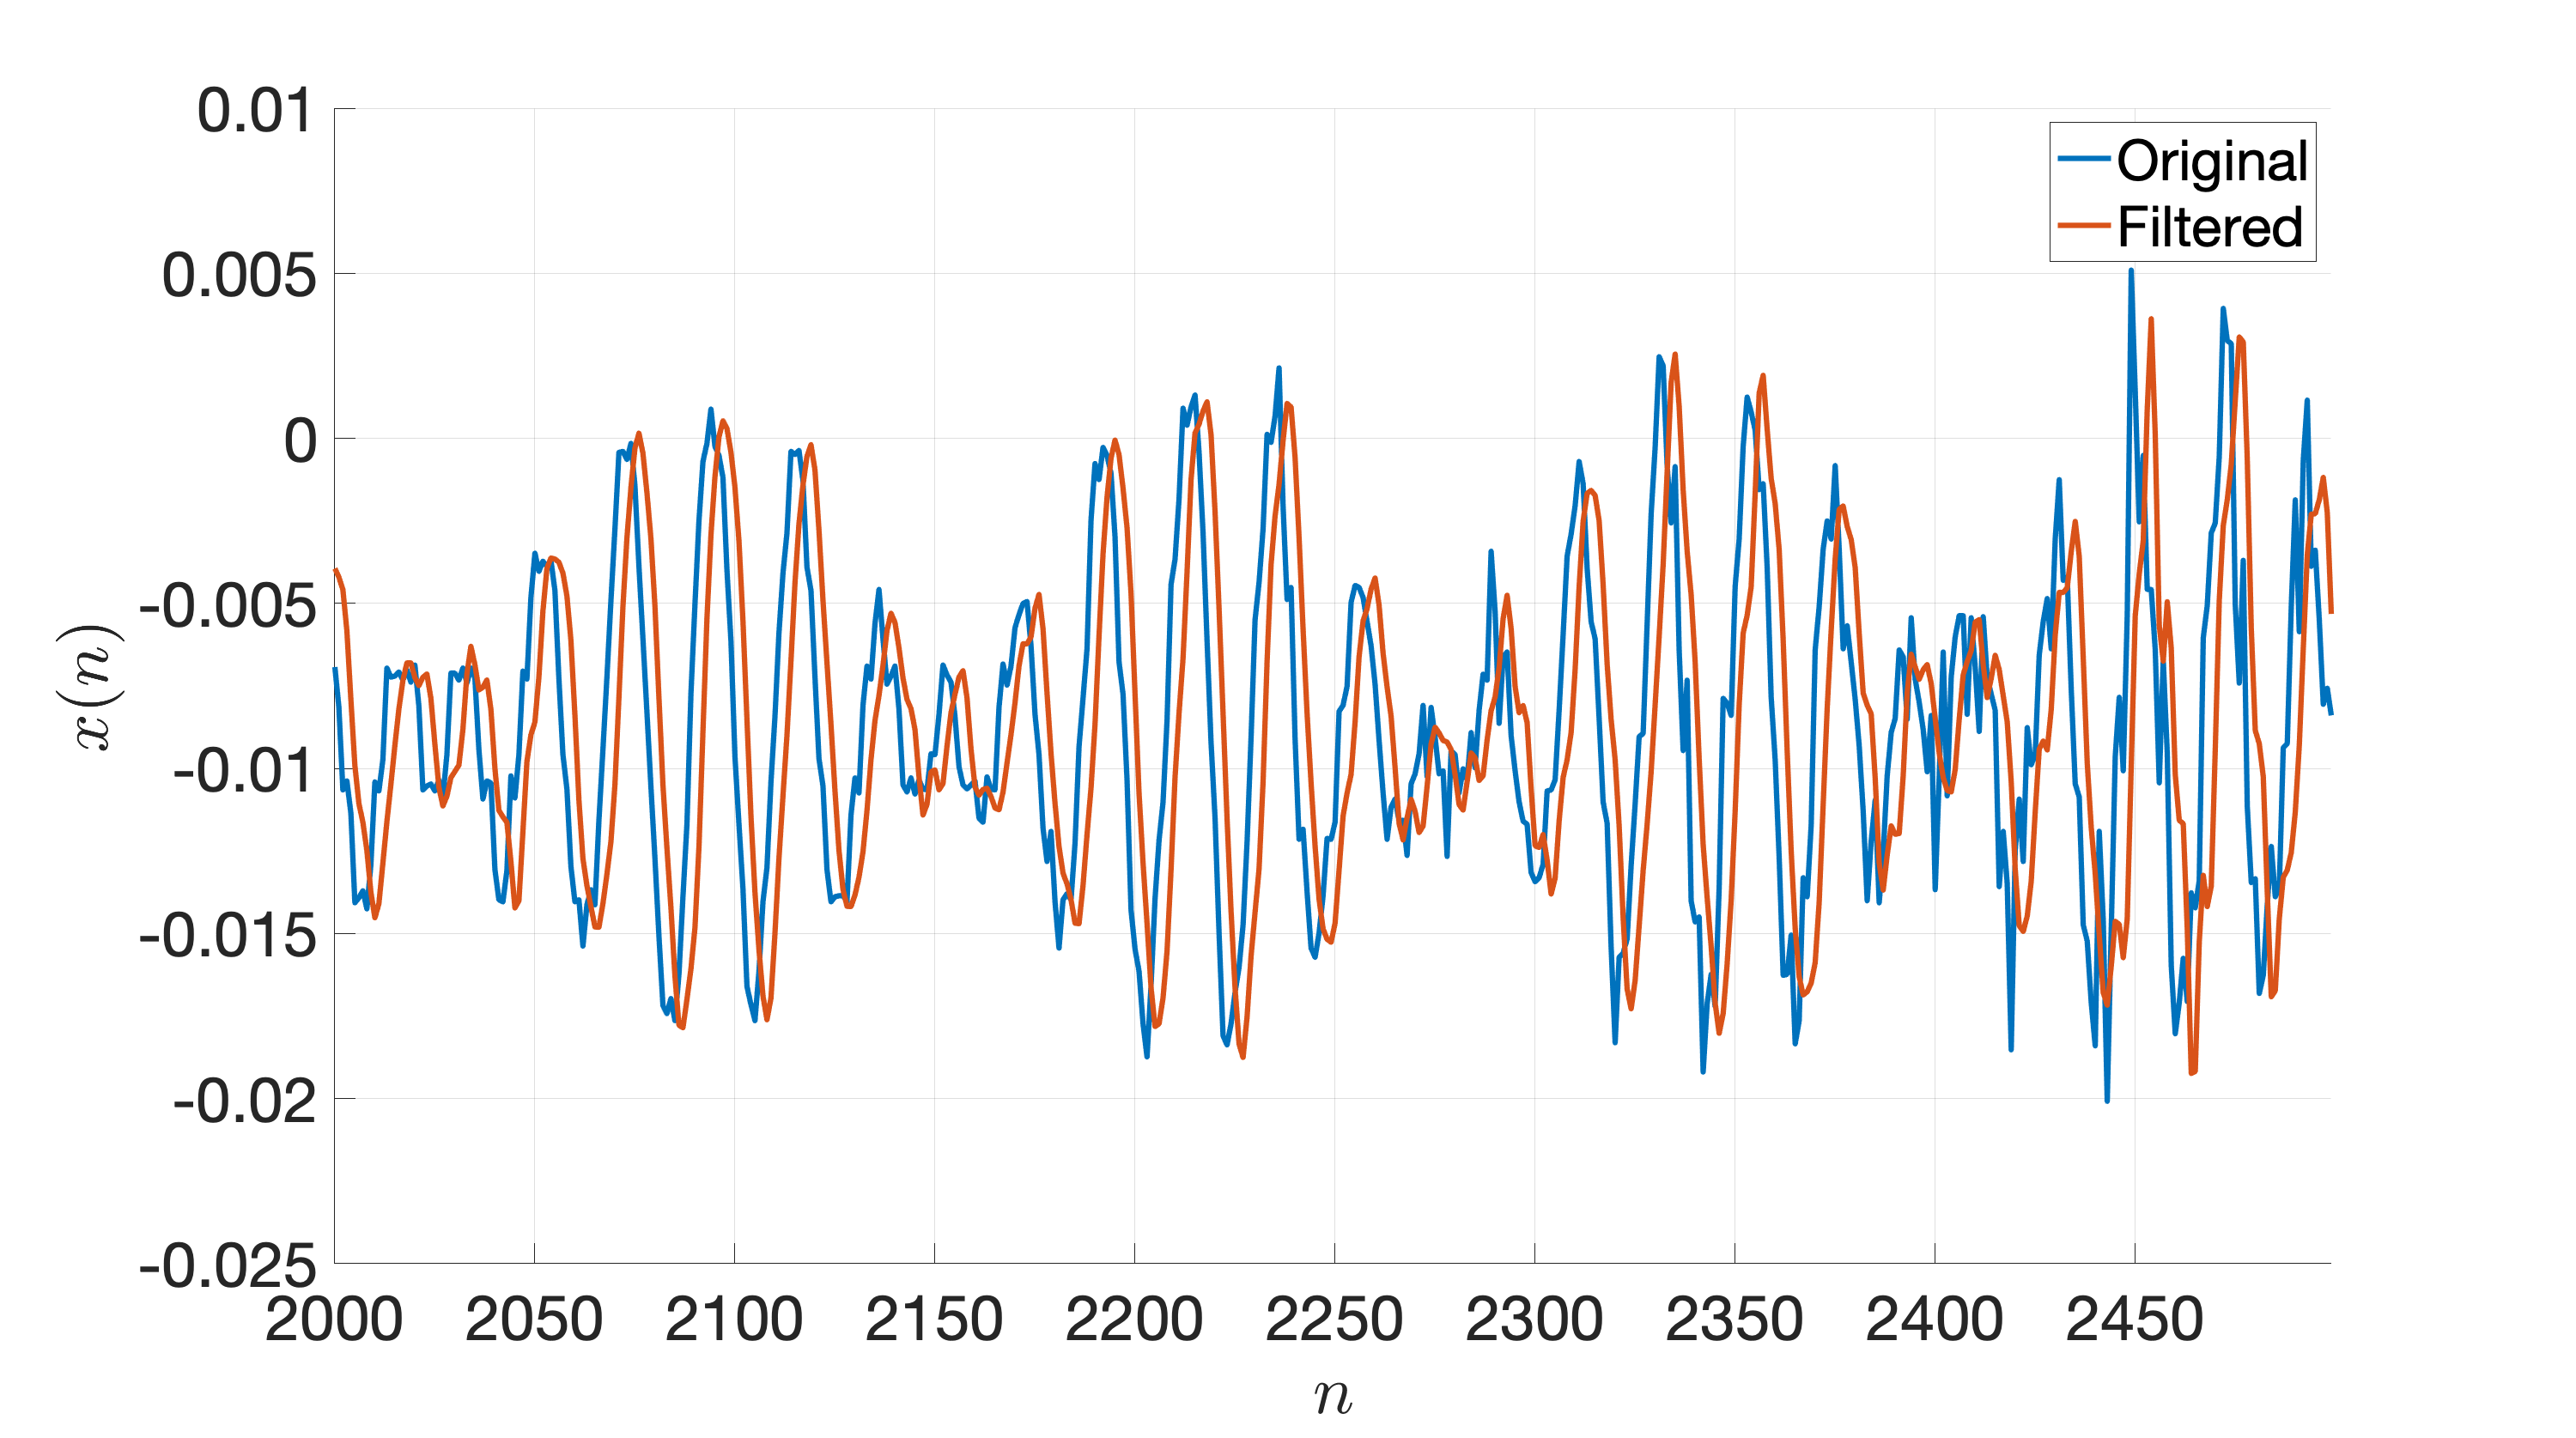
\includegraphics[width= 1.1\textwidth]{figures/R2c_zoomNormal.png}
	\caption{Filtered signal.}
	\label{fig:R2c_zoomNormal}
\end{minipage}
\end{figure}

\subsection{R2.d) Analysis of the filtered signal in the frequency domain}
Fig. \ref{fig:R2d} shows the comparison of the magnitude spectra of the original and filtered signals. As expected from the analysis of the gain of the filter (represented in Fig. \ref{fig:R2a_gain}), the components of the signal with frequency greater than the cutoff frequency (represented in Fig. \ref{fig:R2d} by a vertical dashed line) are attenuated. Nevertheless, given that the magnitude spectrum of the impulsive noise is spread evenly across all frequencies, it is evident that with this filter only a portion of the noise is attenuated. It is also important to remark, that noiseless components of higher frequencies are also attenuated contributing to the distortion and loss of sharpness in the sound of the filtered signal. Furthermore, Fig. \ref{fig:Red_spectrogram} shows the spectrogram of the filtered signal for the segment of Fig. \ref{fig:R1b}. As put forward previously, the constant power vertical noise of the lines remain unchanged for lower frequencies, thus this filter was not able to filter the signal adequately.

\begin{figure}[htbp]
	\centering
	\begin{minipage}[b]{.49\textwidth}
		\centering
		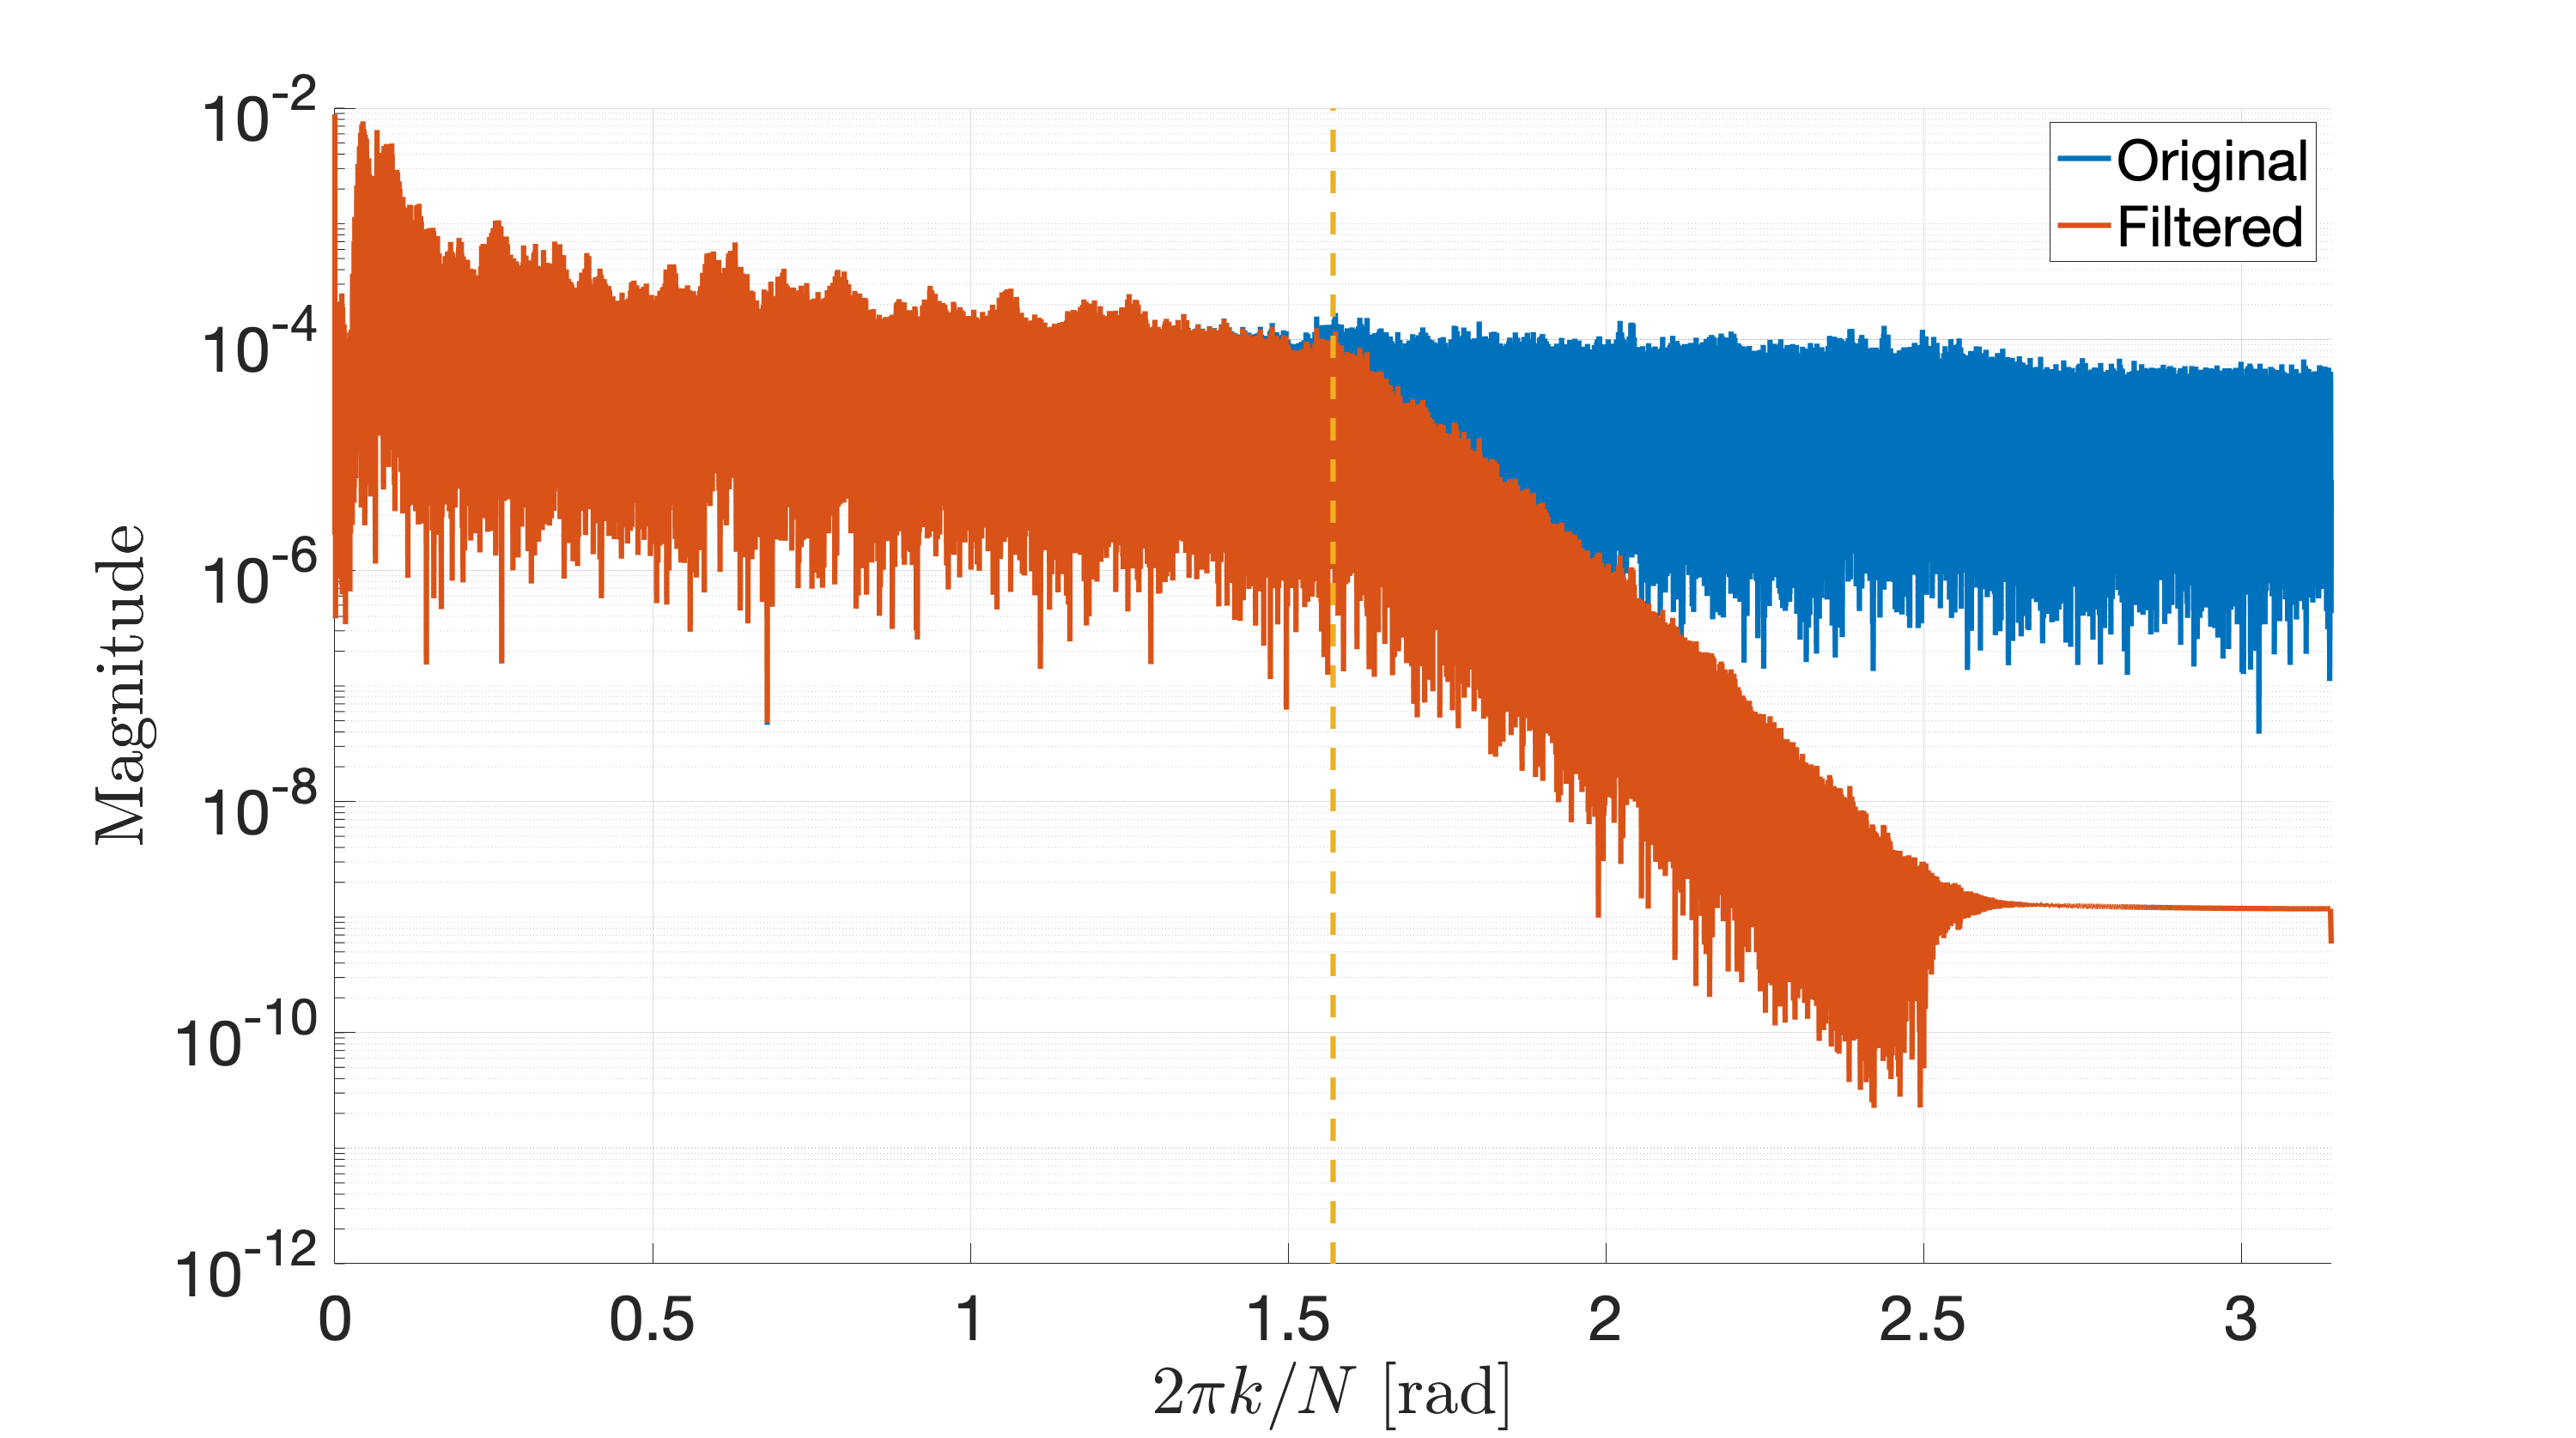
\includegraphics[width= 1.1\textwidth]{figures/R2d.png}
		\caption{Magnitude spectrum of the original and filtered sound signals.}
		\label{fig:R2d}
	\end{minipage}
	\hfill
	\begin{minipage}[b]{.49\textwidth}
		\centering
		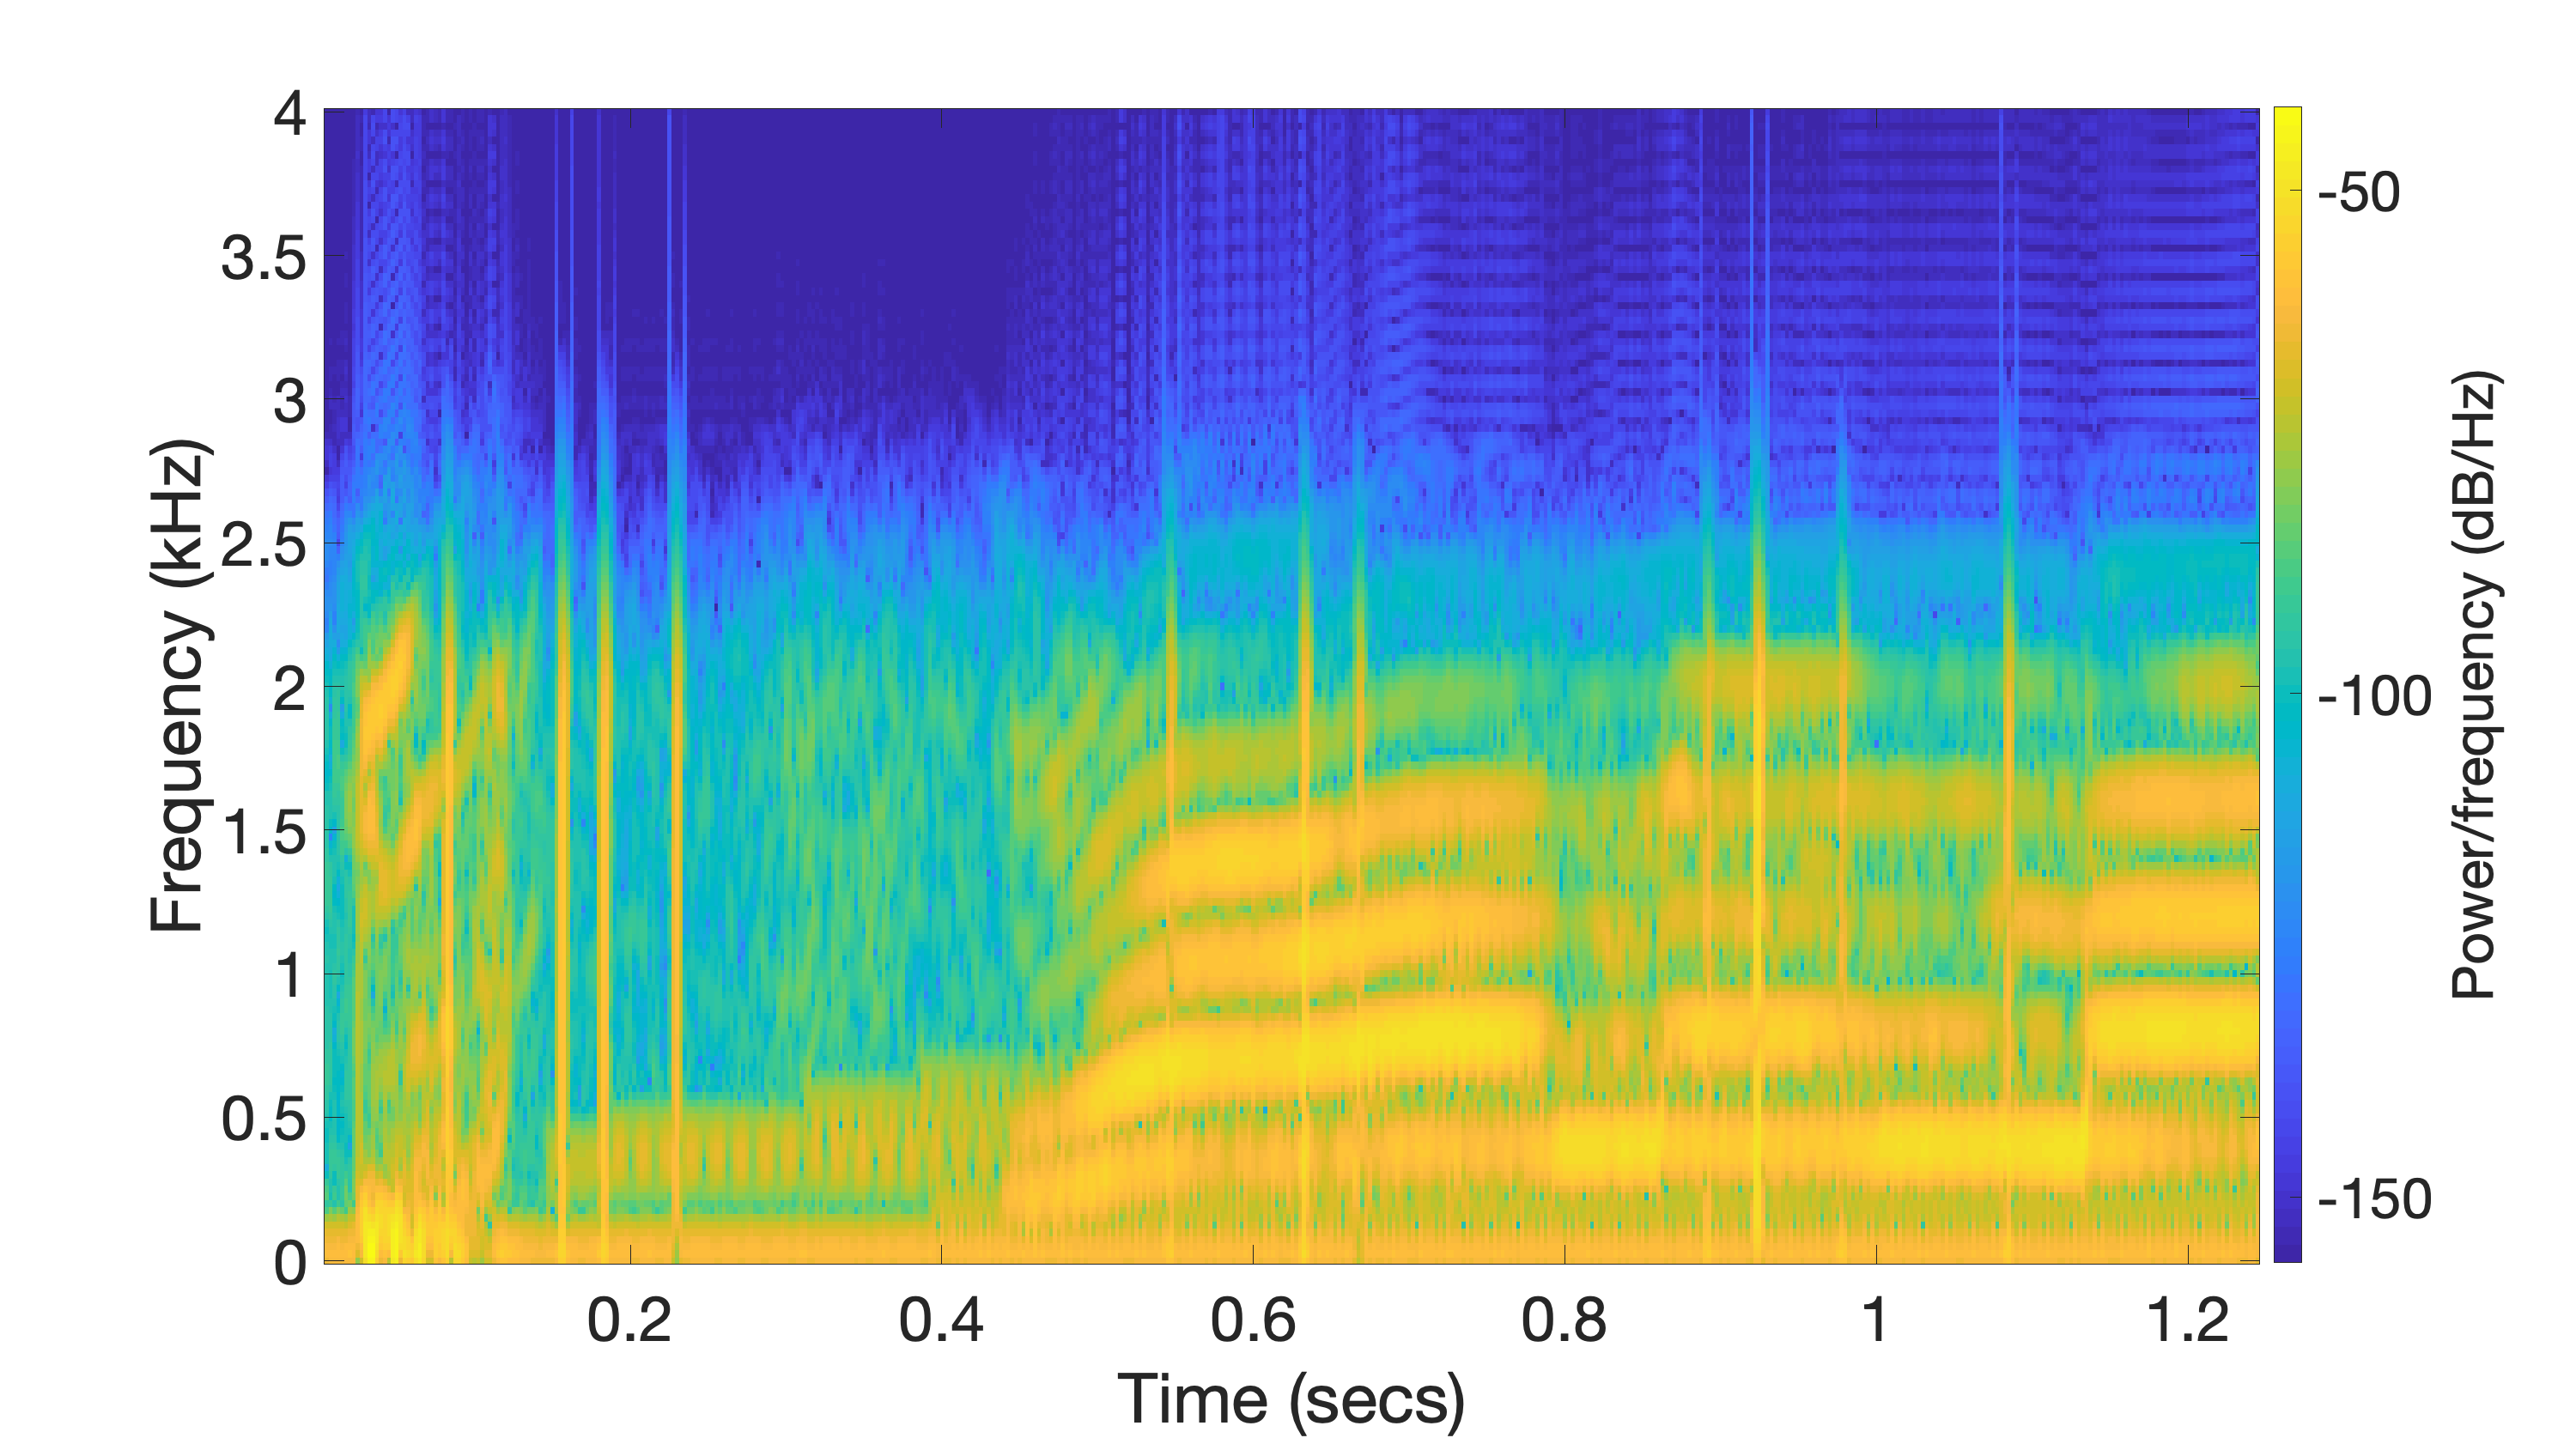
\includegraphics[width= 1.1\textwidth]{figures/R2d_spectrogram.png}
		\caption{Spectrogram of the filtered signal the segment of Fig. \ref{fig:R1b}.}
		\label{fig:Red_spectrogram}
	\end{minipage}
\end{figure}

\subsection{R2.e) Listen to the filtered signal}
Listening to the filtered signal it is possible to conclude that the attenuation on the impulsive noise is very unsatisfactory, given that the noise impulses are still very clear and loud. Furthermore, there is a loss of sharpness in the song because of the phenomena put forward in the two previous subsections.

\subsection{R2.a) Improve Butterworth low-pass filter}
The Butterworth filter operates on frequency, but as seen in Section \ref{sec:R1}, it is very difficult to identify and isolate the noise in the frequency domain. It is thus expected that the performance of such a filter is poor, as noticed so far. Given that magnitude spectrum the noise impulses are spread evenly across all frequencies the only way of attenuating the impulsive noise is to decrease the cutoff frequency of the filter. This solution results, however, in the degradation of the quality of the song. Using this filter for this particular noise reduces to a trade-off between degradation of quality and noise attenuation. Synthesizing a filter with cutoff frequency $\omega_{co} = \pi/4$, the filtered signal is characterized in Figs. \ref{fig:Rfc}--\ref{fig:R2f_spectrogram}. 

First, it is seen in Fig. \ref{fig:Rfc} that although the noise impulses are more attenuated in relation to Fig. \ref{fig:R2c}. However, they are still very significant. This is expected, since a larger portion of component of the constant magnitude spectrum of the noise signal was attenuated. However, some segments of the signal which are not corrupted by noise are attenuated and, thus, distorted. Second, in Fig. \ref{fig:R2f_zoomNoise} it is possible to analyze the behavior of the filter after a noise impulse in the time domain. After the noise impulse, as expected, the response of the noiseless signal is still superimposed with the impulse response of the filter, which is still similar to the response of a under-damped second order system with a lower natural frequency. Third, in Fig. \ref{fig:R2c_zoomNormal} it is possible to notice that the delay introduced by the filter increased. Fourth, from Figs. \ref{fig:R2f} and \ref{fig:R2f_spectrogram}, given that the magnitude spectrum of the impulsive noise is spread evenly across all frequencies, it is evident that with this filter still only a portion, albeit larger, of the noise is attenuated. It is also important to remark, that noiseless components of the signal are even more also attenuated contributing to a greater distortion and loss of sharpness in the sound of the filtered signal.
 
\begin{figure}[htbp]
	\centering
	\begin{minipage}[b]{.49\textwidth}
		\centering
		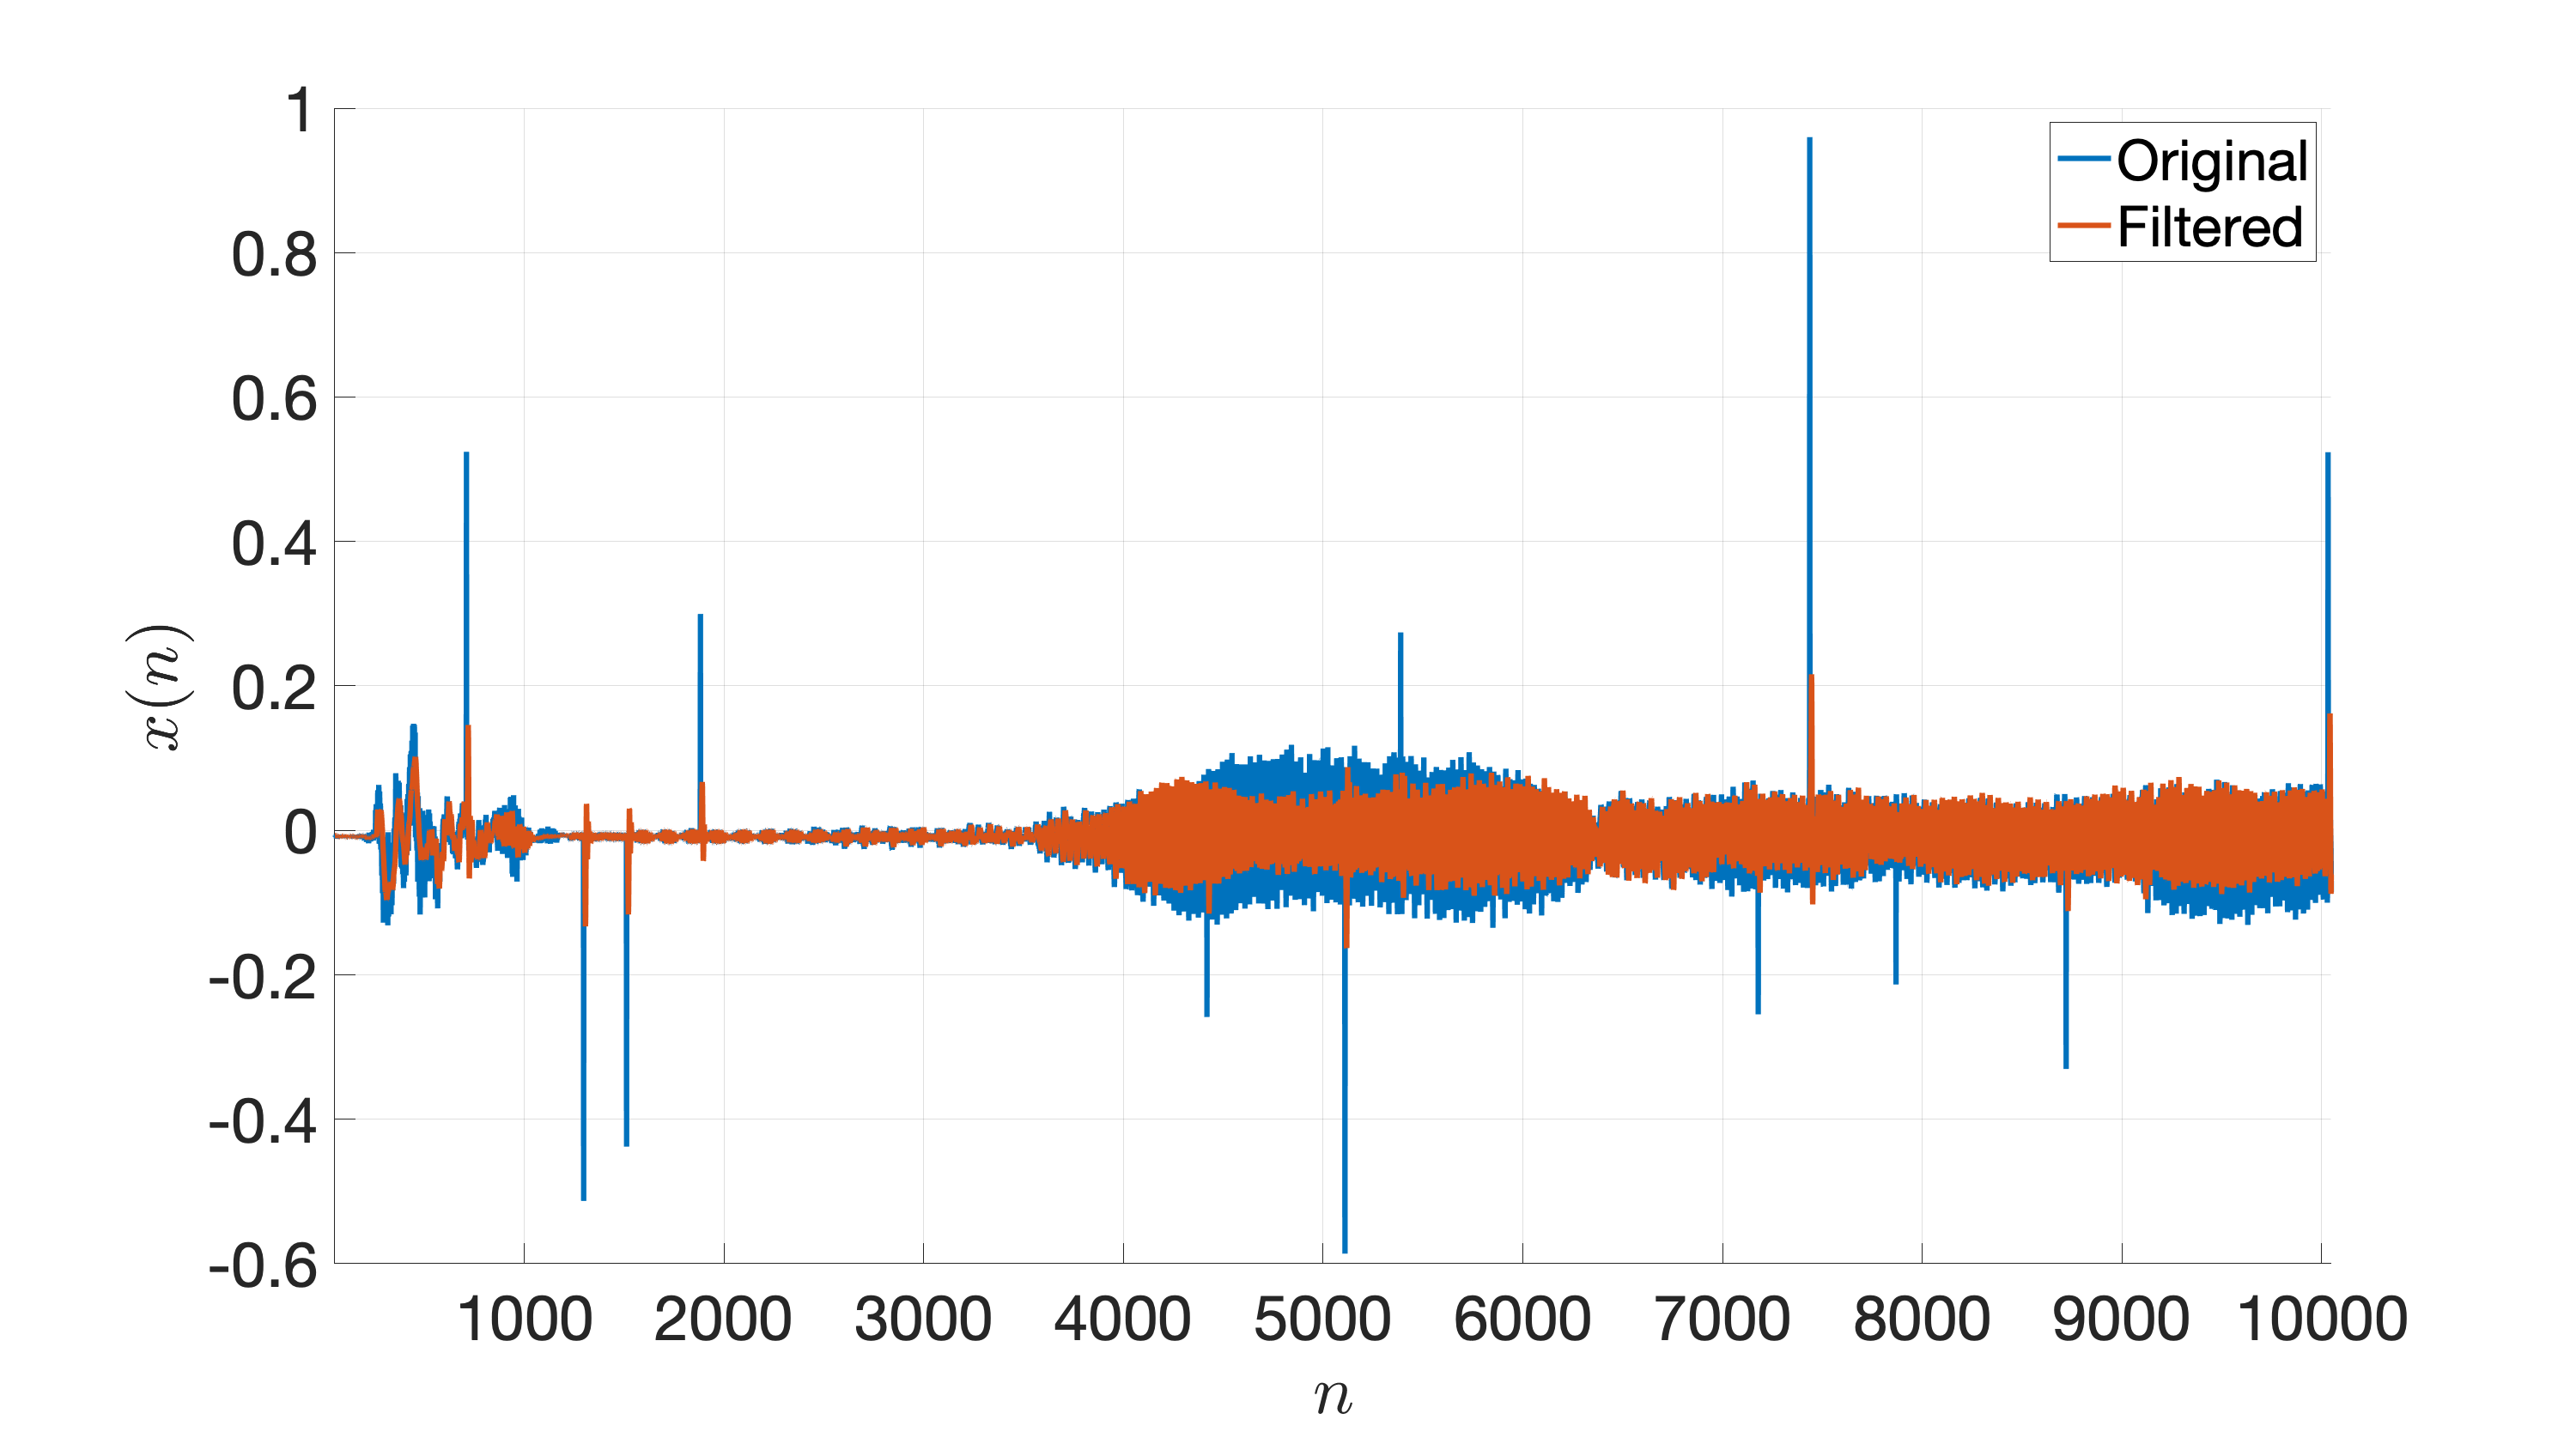
\includegraphics[width= 1.1\textwidth]{figures/R2f_zoomOut.png}
		\caption{Filtered signal.}
		\label{fig:Rfc}
	\end{minipage}
	\hfill
	\begin{minipage}[b]{.49\textwidth}
		\centering
		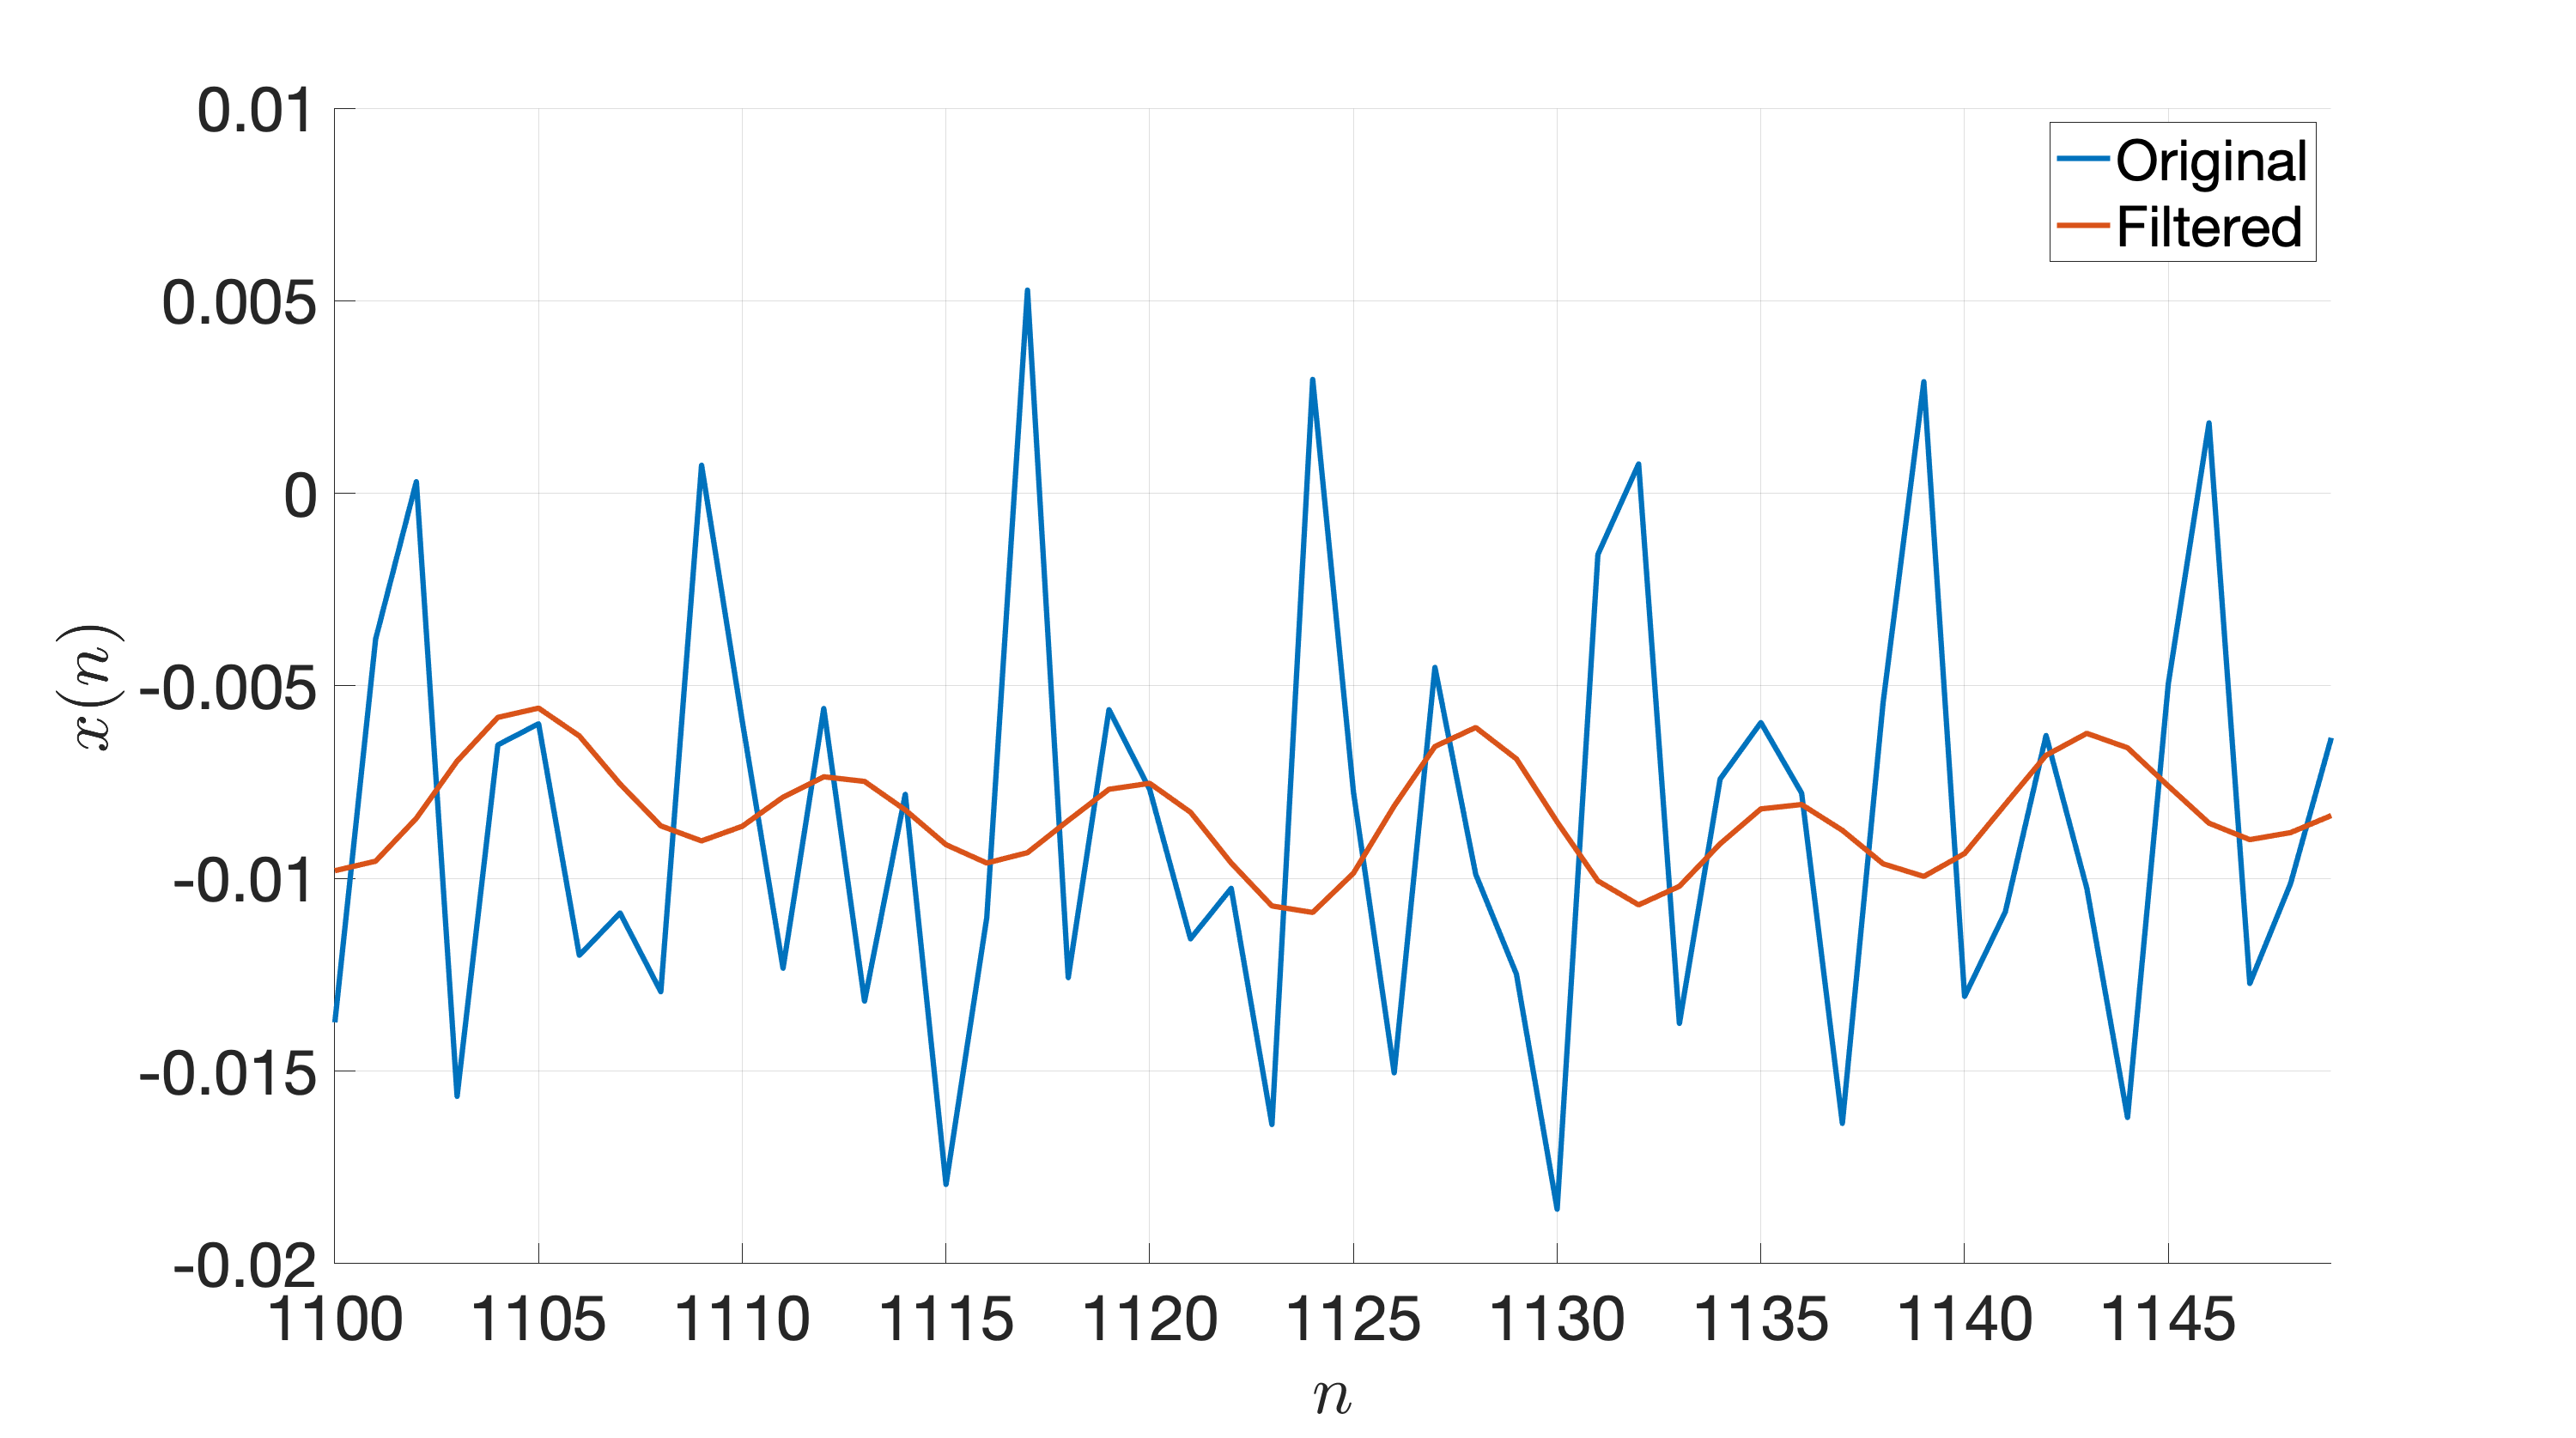
\includegraphics[width= 1.1\textwidth]{figures/R2f_smallAmp.png}
		\caption{Filtered signal.}
		\label{fig:R2f_smallAmp}
	\end{minipage}
	\begin{minipage}[b]{.49\textwidth}
		\centering
		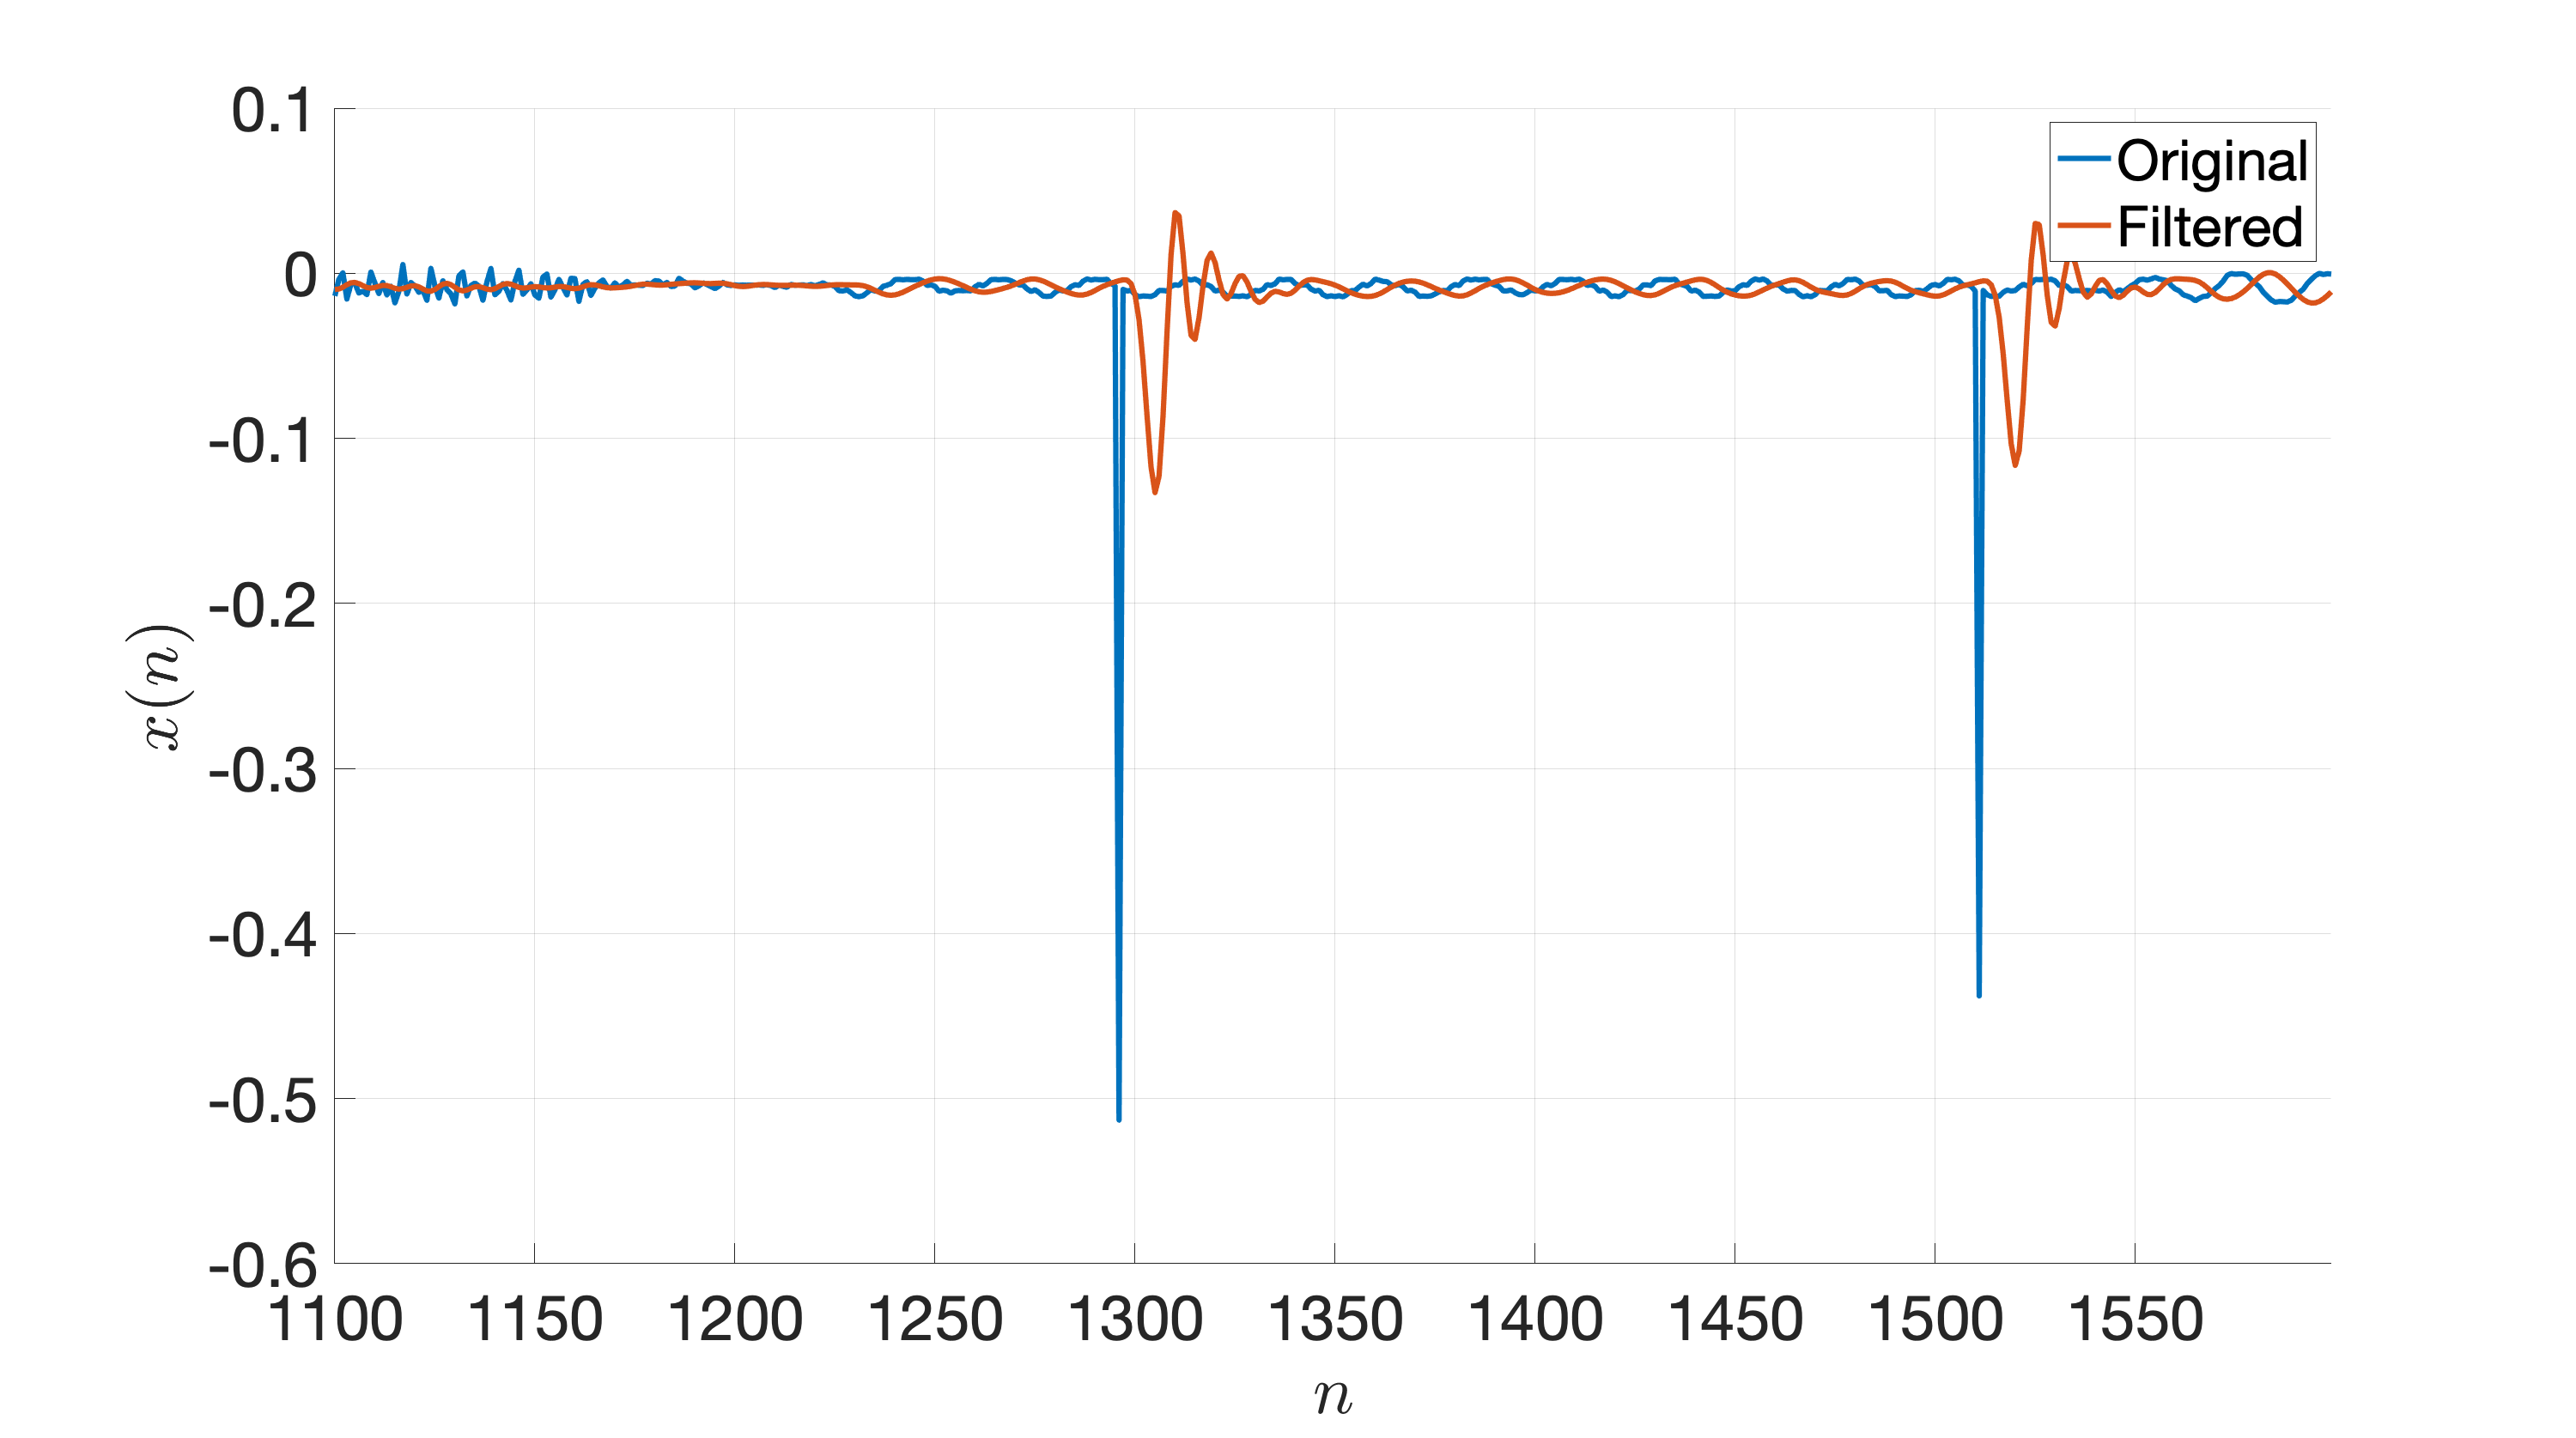
\includegraphics[width= 1.1\textwidth]{figures/R2f_zoomNoise.png}
		\caption{Filtered signal.}
		\label{fig:R2f_zoomNoise}
	\end{minipage}
	\hfill
	\begin{minipage}[b]{.49\textwidth}
		\centering
		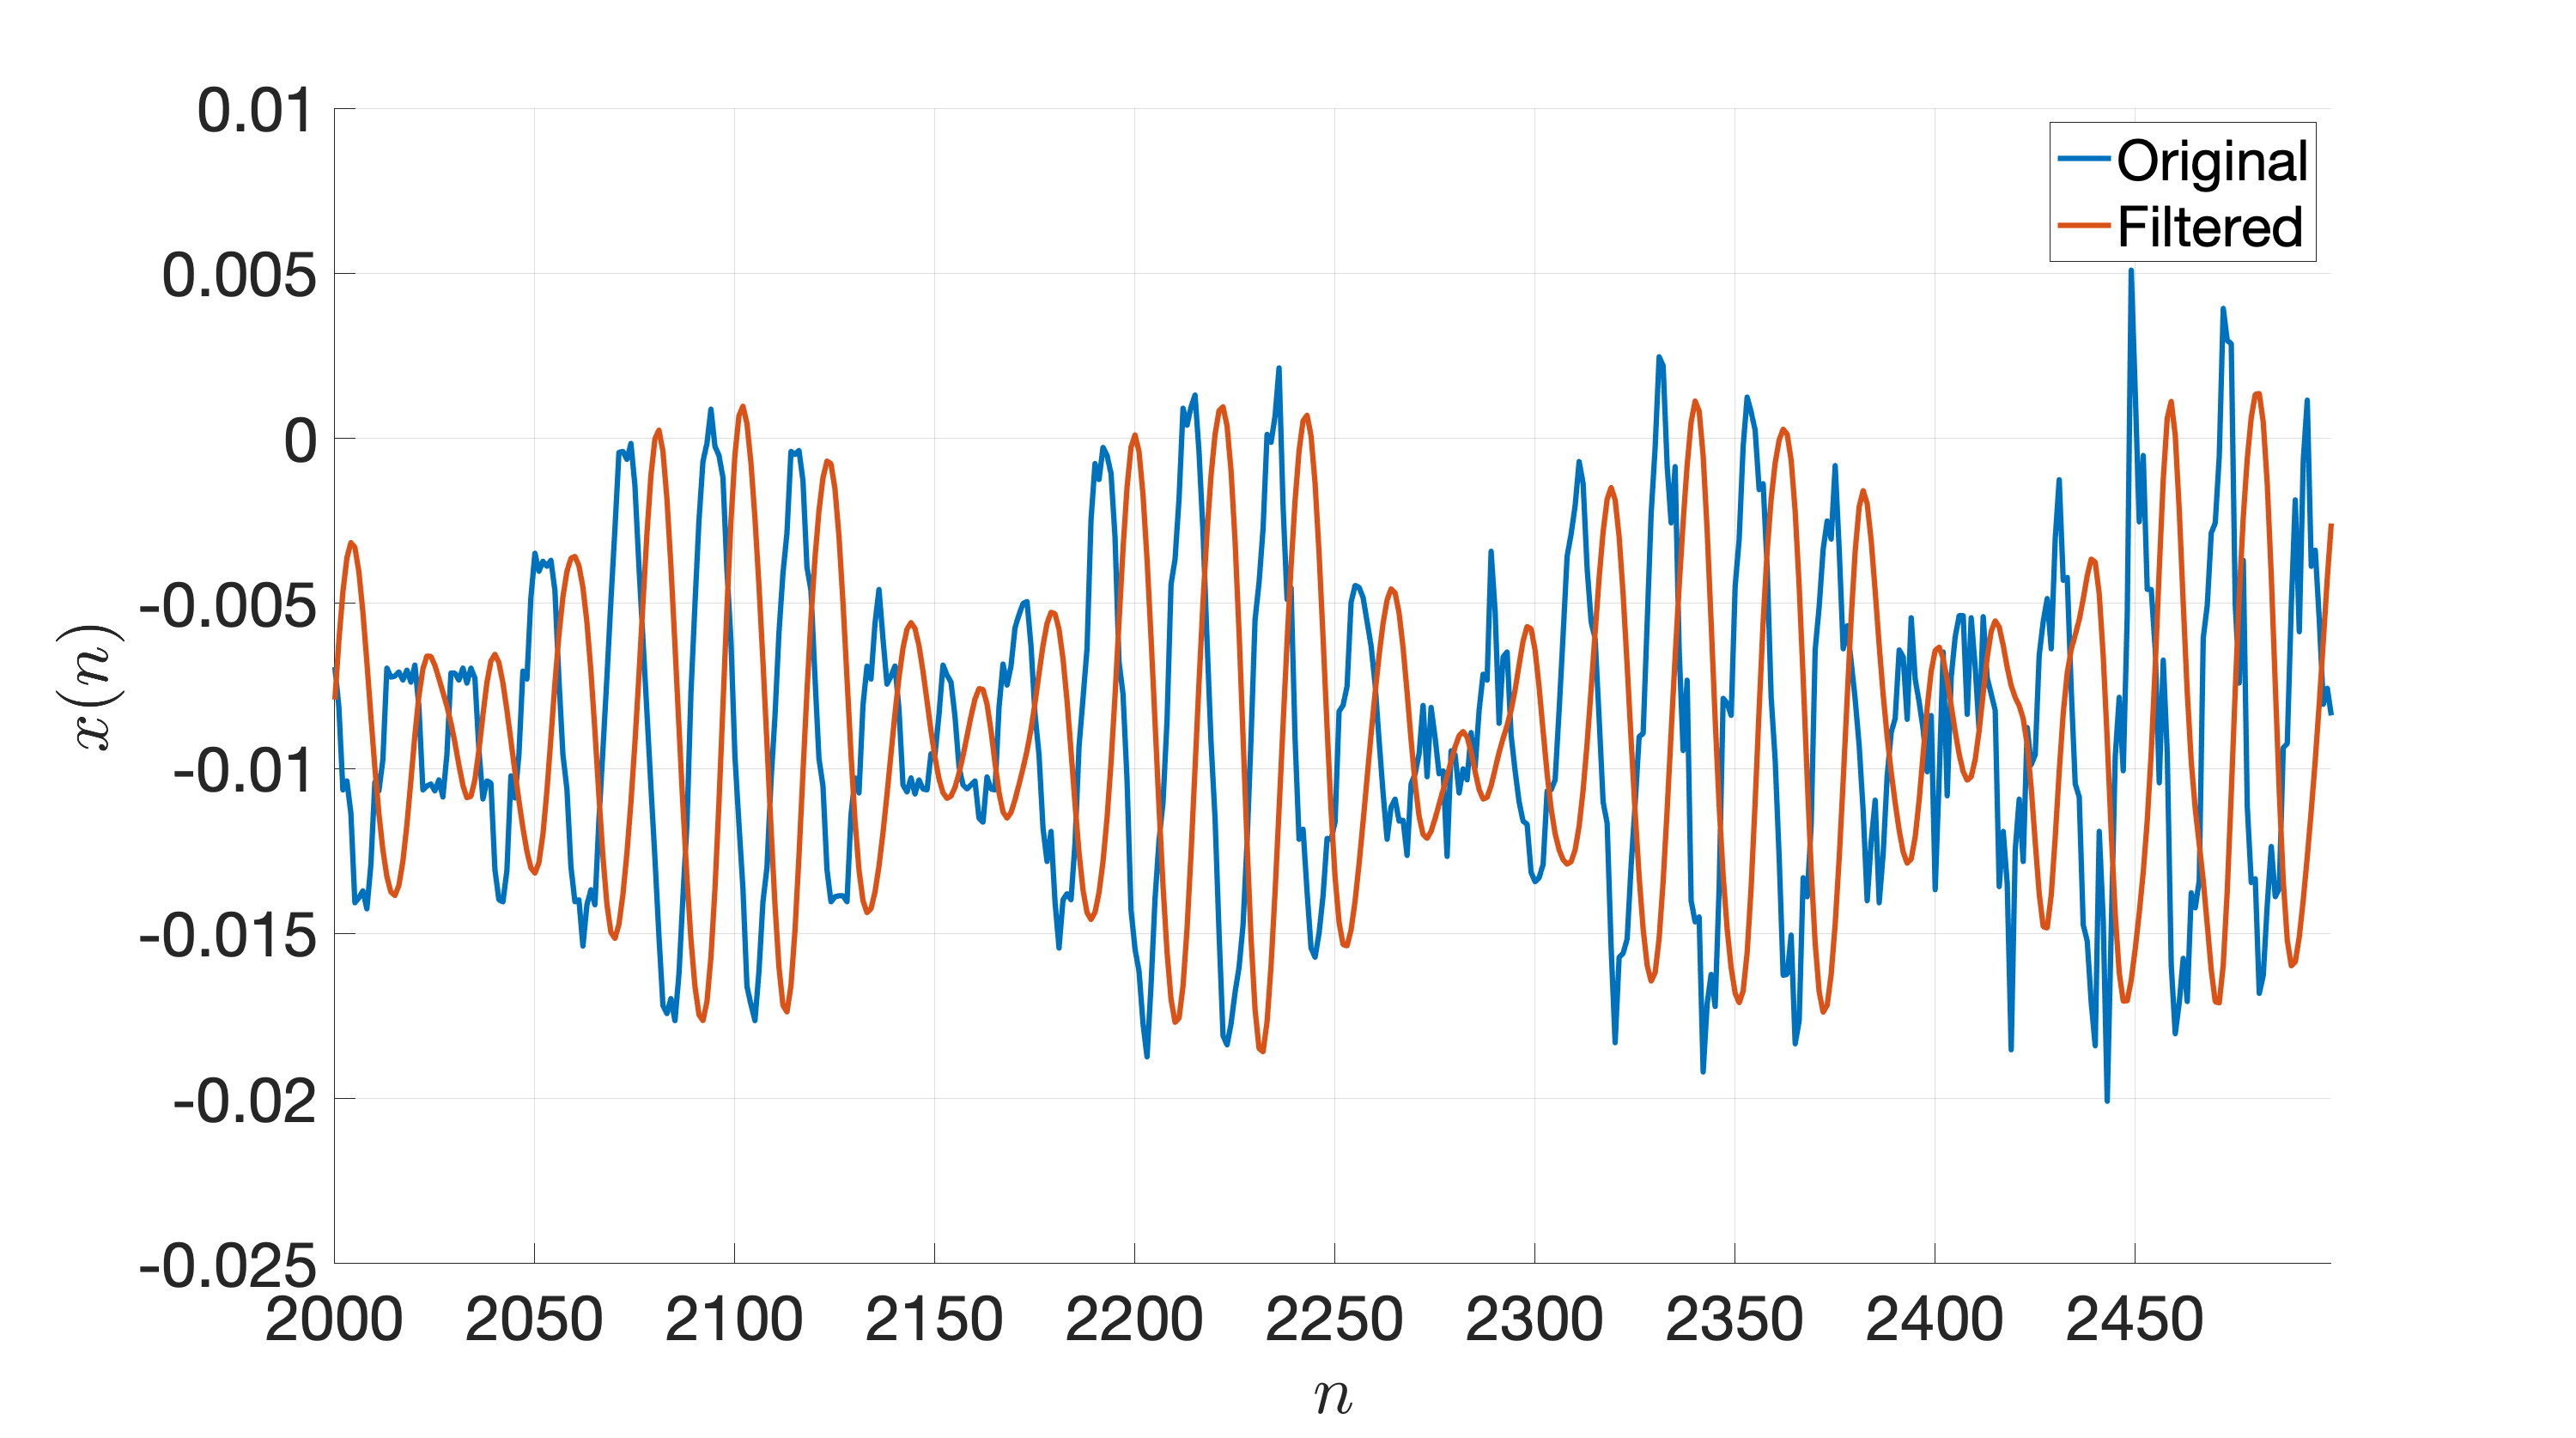
\includegraphics[width= 1.1\textwidth]{figures/R2f_zoomNormal.png}
		\caption{Filtered signal.}
		\label{fig:R2f_zoomNormal}
	\end{minipage}
\begin{minipage}[b]{.49\textwidth}
	\centering
	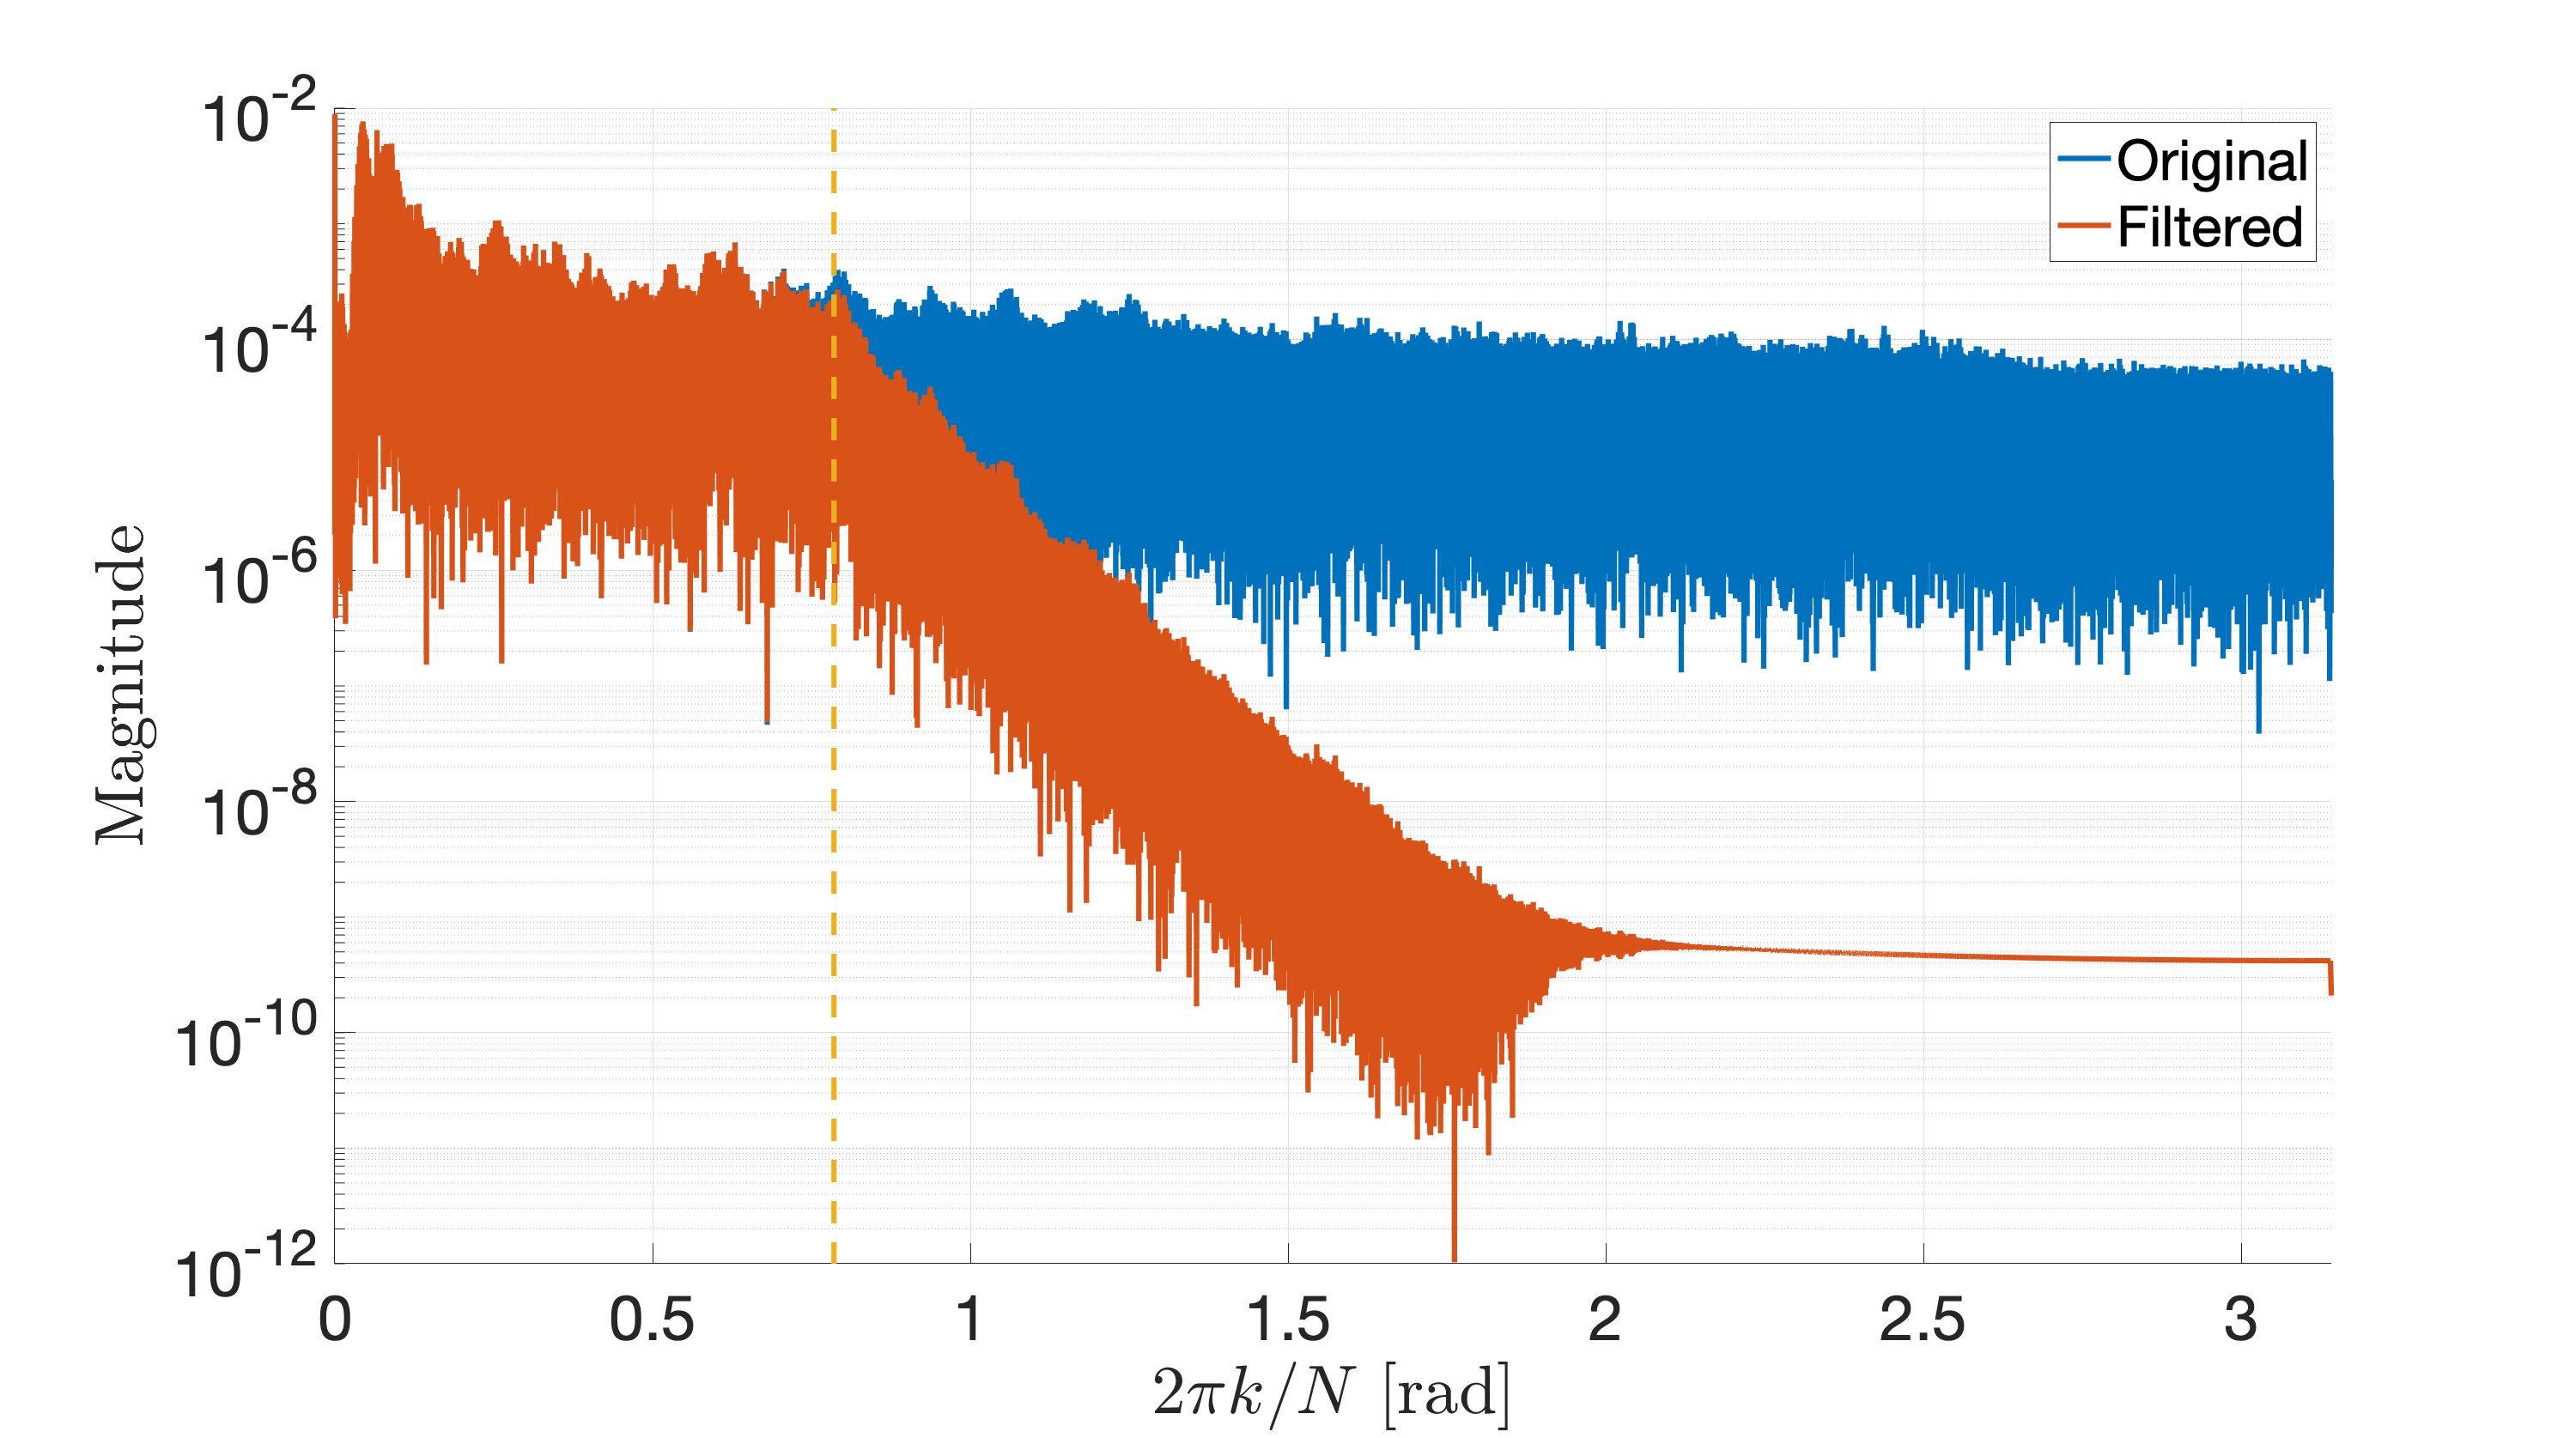
\includegraphics[width= 1.1\textwidth]{figures/R2f_spectra.png}
	\caption{Magnitude spectrum of the original and filtered sound signals.}
	\label{fig:R2f}
\end{minipage}
\hfill
\begin{minipage}[b]{.49\textwidth}
	\centering
	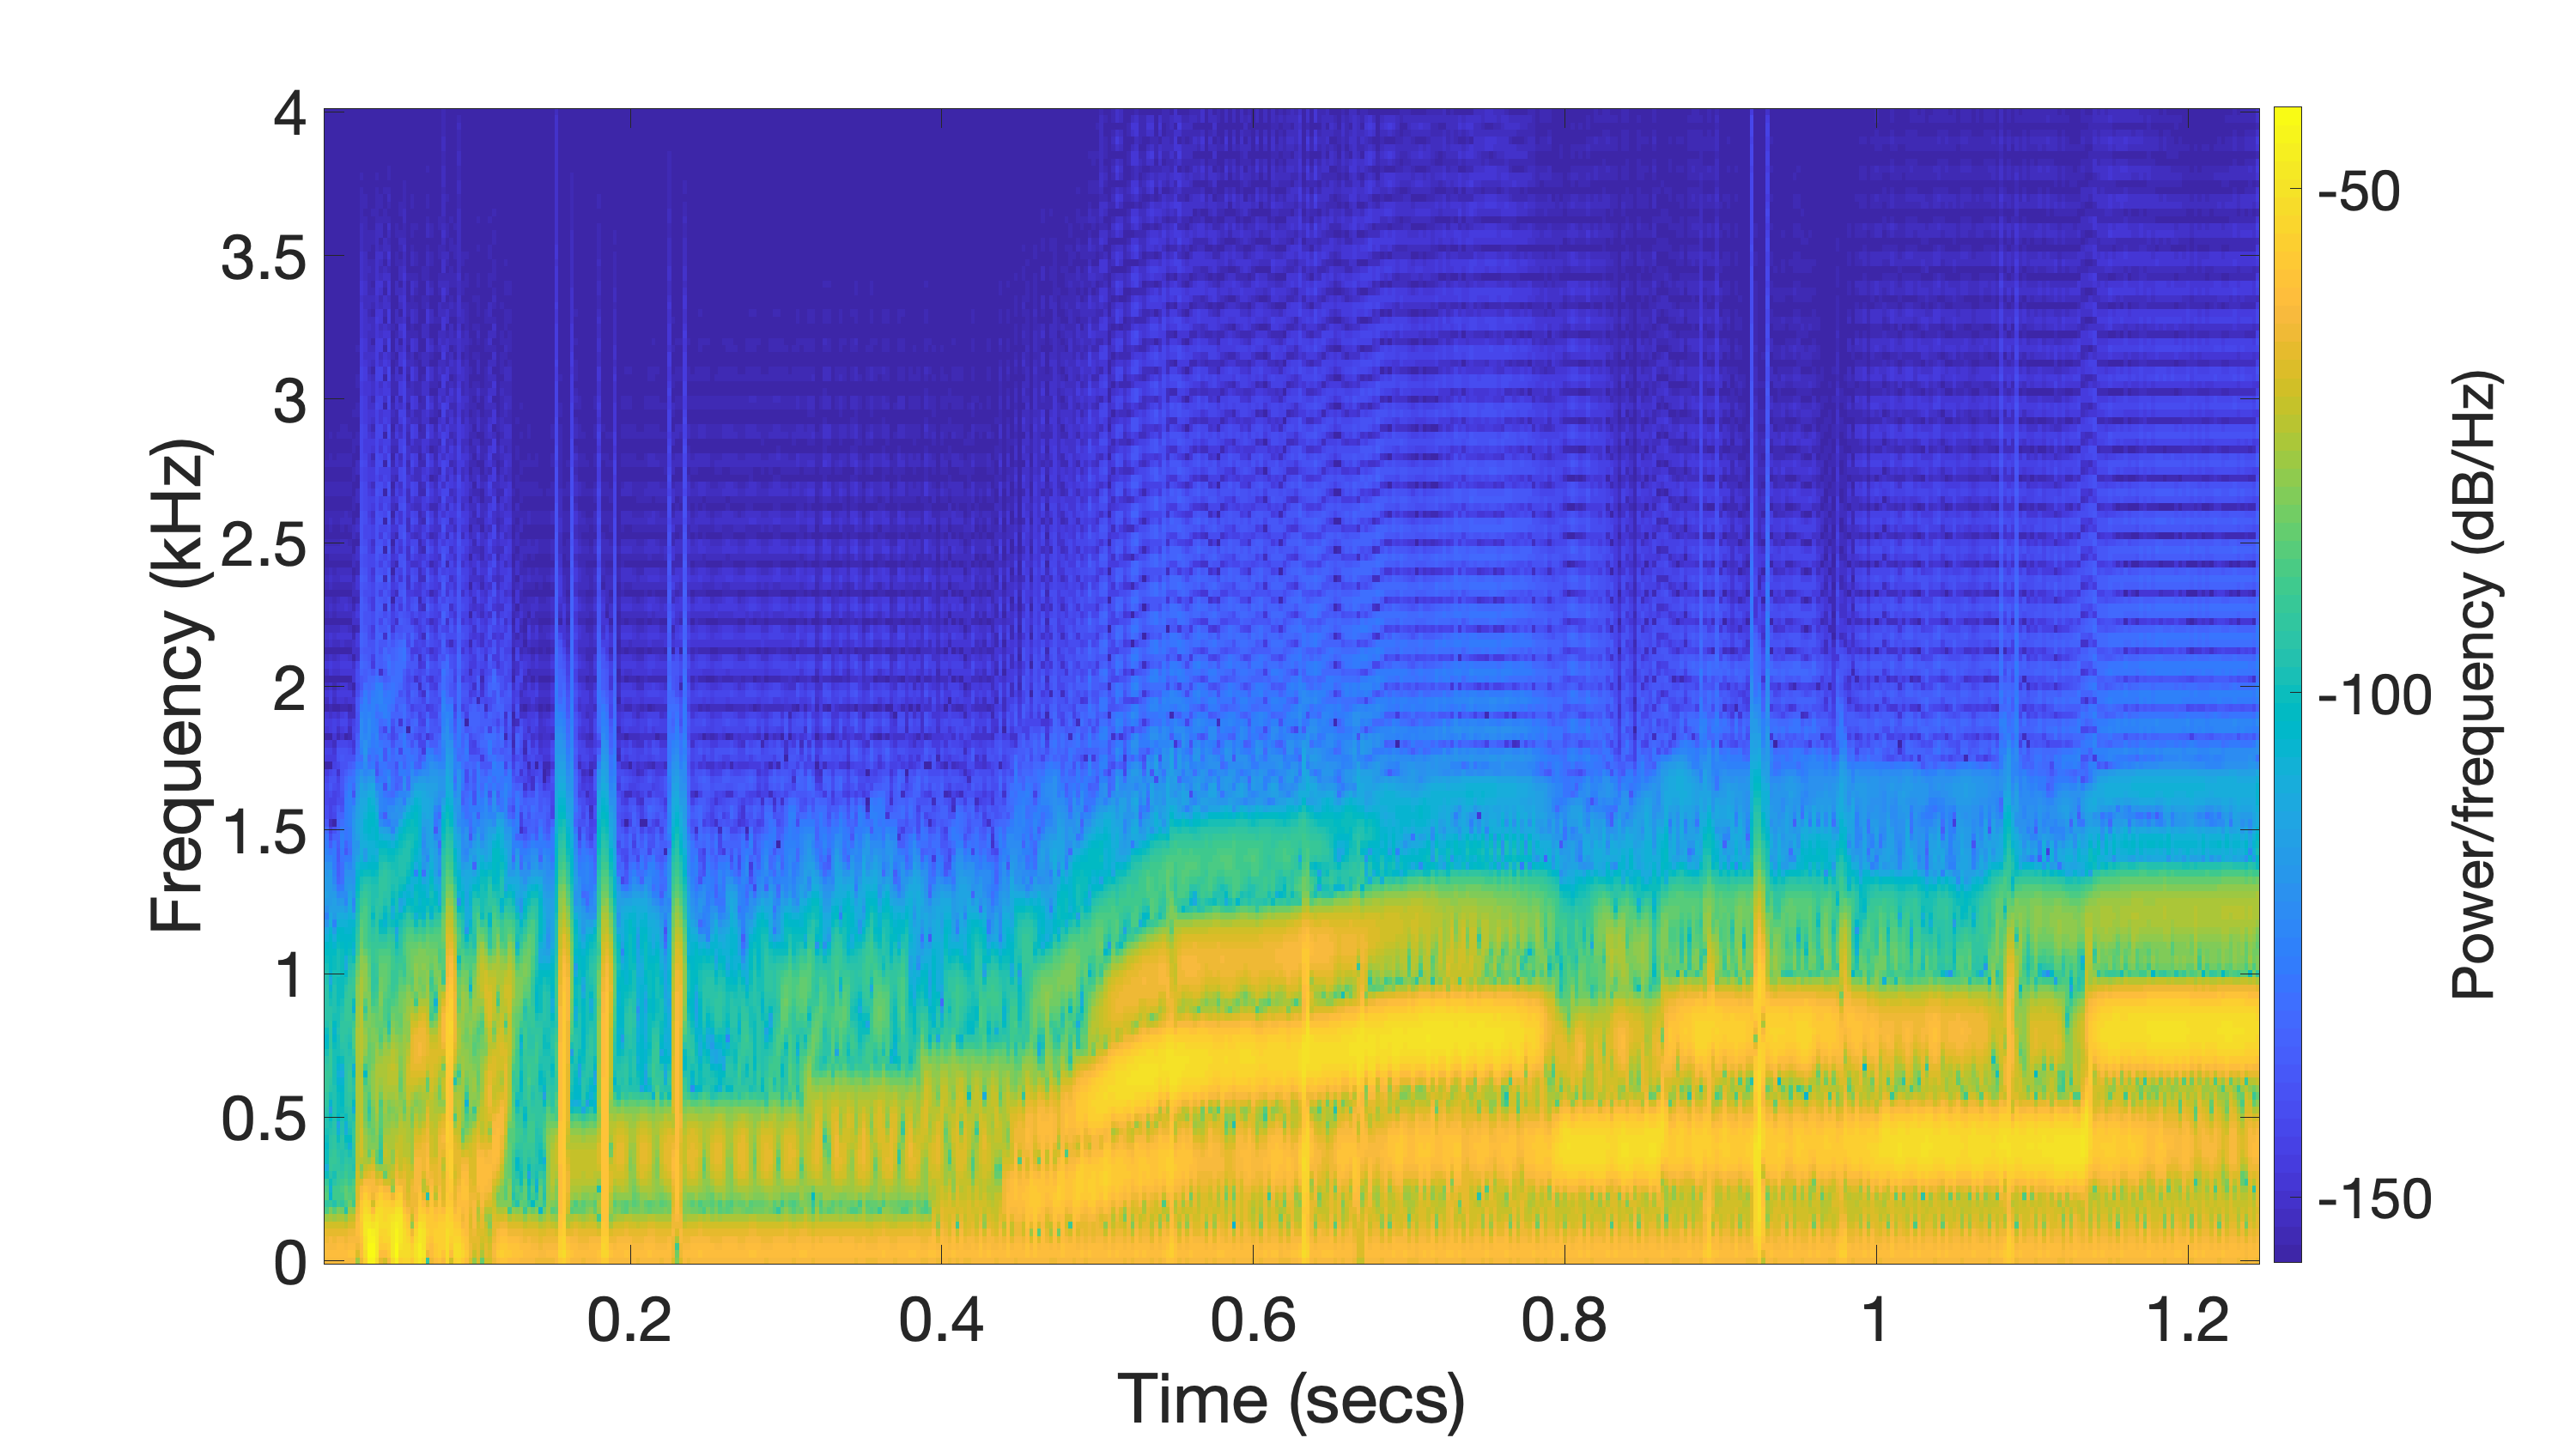
\includegraphics[width= 1.1\textwidth]{figures/R2f_spectrogram.png}
	\caption{Spectrogram of the filtered signal the segment of Fig. \ref{fig:R1b}.}
	\label{fig:R2f_spectrogram}
\end{minipage}
\end{figure}

\begin{comment}




\subsection{R1.a),R1.b) Synthetic signal}\label{sec:R1a}
First of all, the signal $x(n)$ of duration $M=512$ was created, as given by 
\begin{equation}\label{eq:defx}
	x(n) = 5\cos(\omega_0 n +1)+2\cos(2\omega_0 n +2)+3\cos(5\omega_0 n +3)\:,
\end{equation}
with $\omega_0 = 5.2\times 2\pi/M$ rad. The signal $x(n)$ is presented in Fig. \ref{fig:R1b}. As it is possible to observe from \eqref{eq:defx} and Fig. \ref{fig:R1b}, the signal $x(n)$ is composed of a linear combination three harmonics, whose frequency are integer which are multiples of the lowest frequency $\omega_0$. Note that such angular frequency can be written as a rational fraction of $2\pi$ as $\omega_0 = 2\pi \times 13/1280$.


\subsection{R1.c) Discrete Fourier Transform}

Second of all, the one-sided Discrete Fourier Transform (DFT) of length $N= 512$ of signal $x(n)$ was computed. Figs. \ref{fig:R1c_mag} and \ref{fig:R1c_arg} show the magintude and phase of the one-sided DFT coefficients $X(k)$, repectively, in function of the normalized frequency $\omega = 2\pi k/N$. It is evident that there are 3 peaks of the magnitude of the DFT, each corresponding to an harmonic of signal $x(n)$, as expected.

\begin{figure}[htbp]
	\centering
	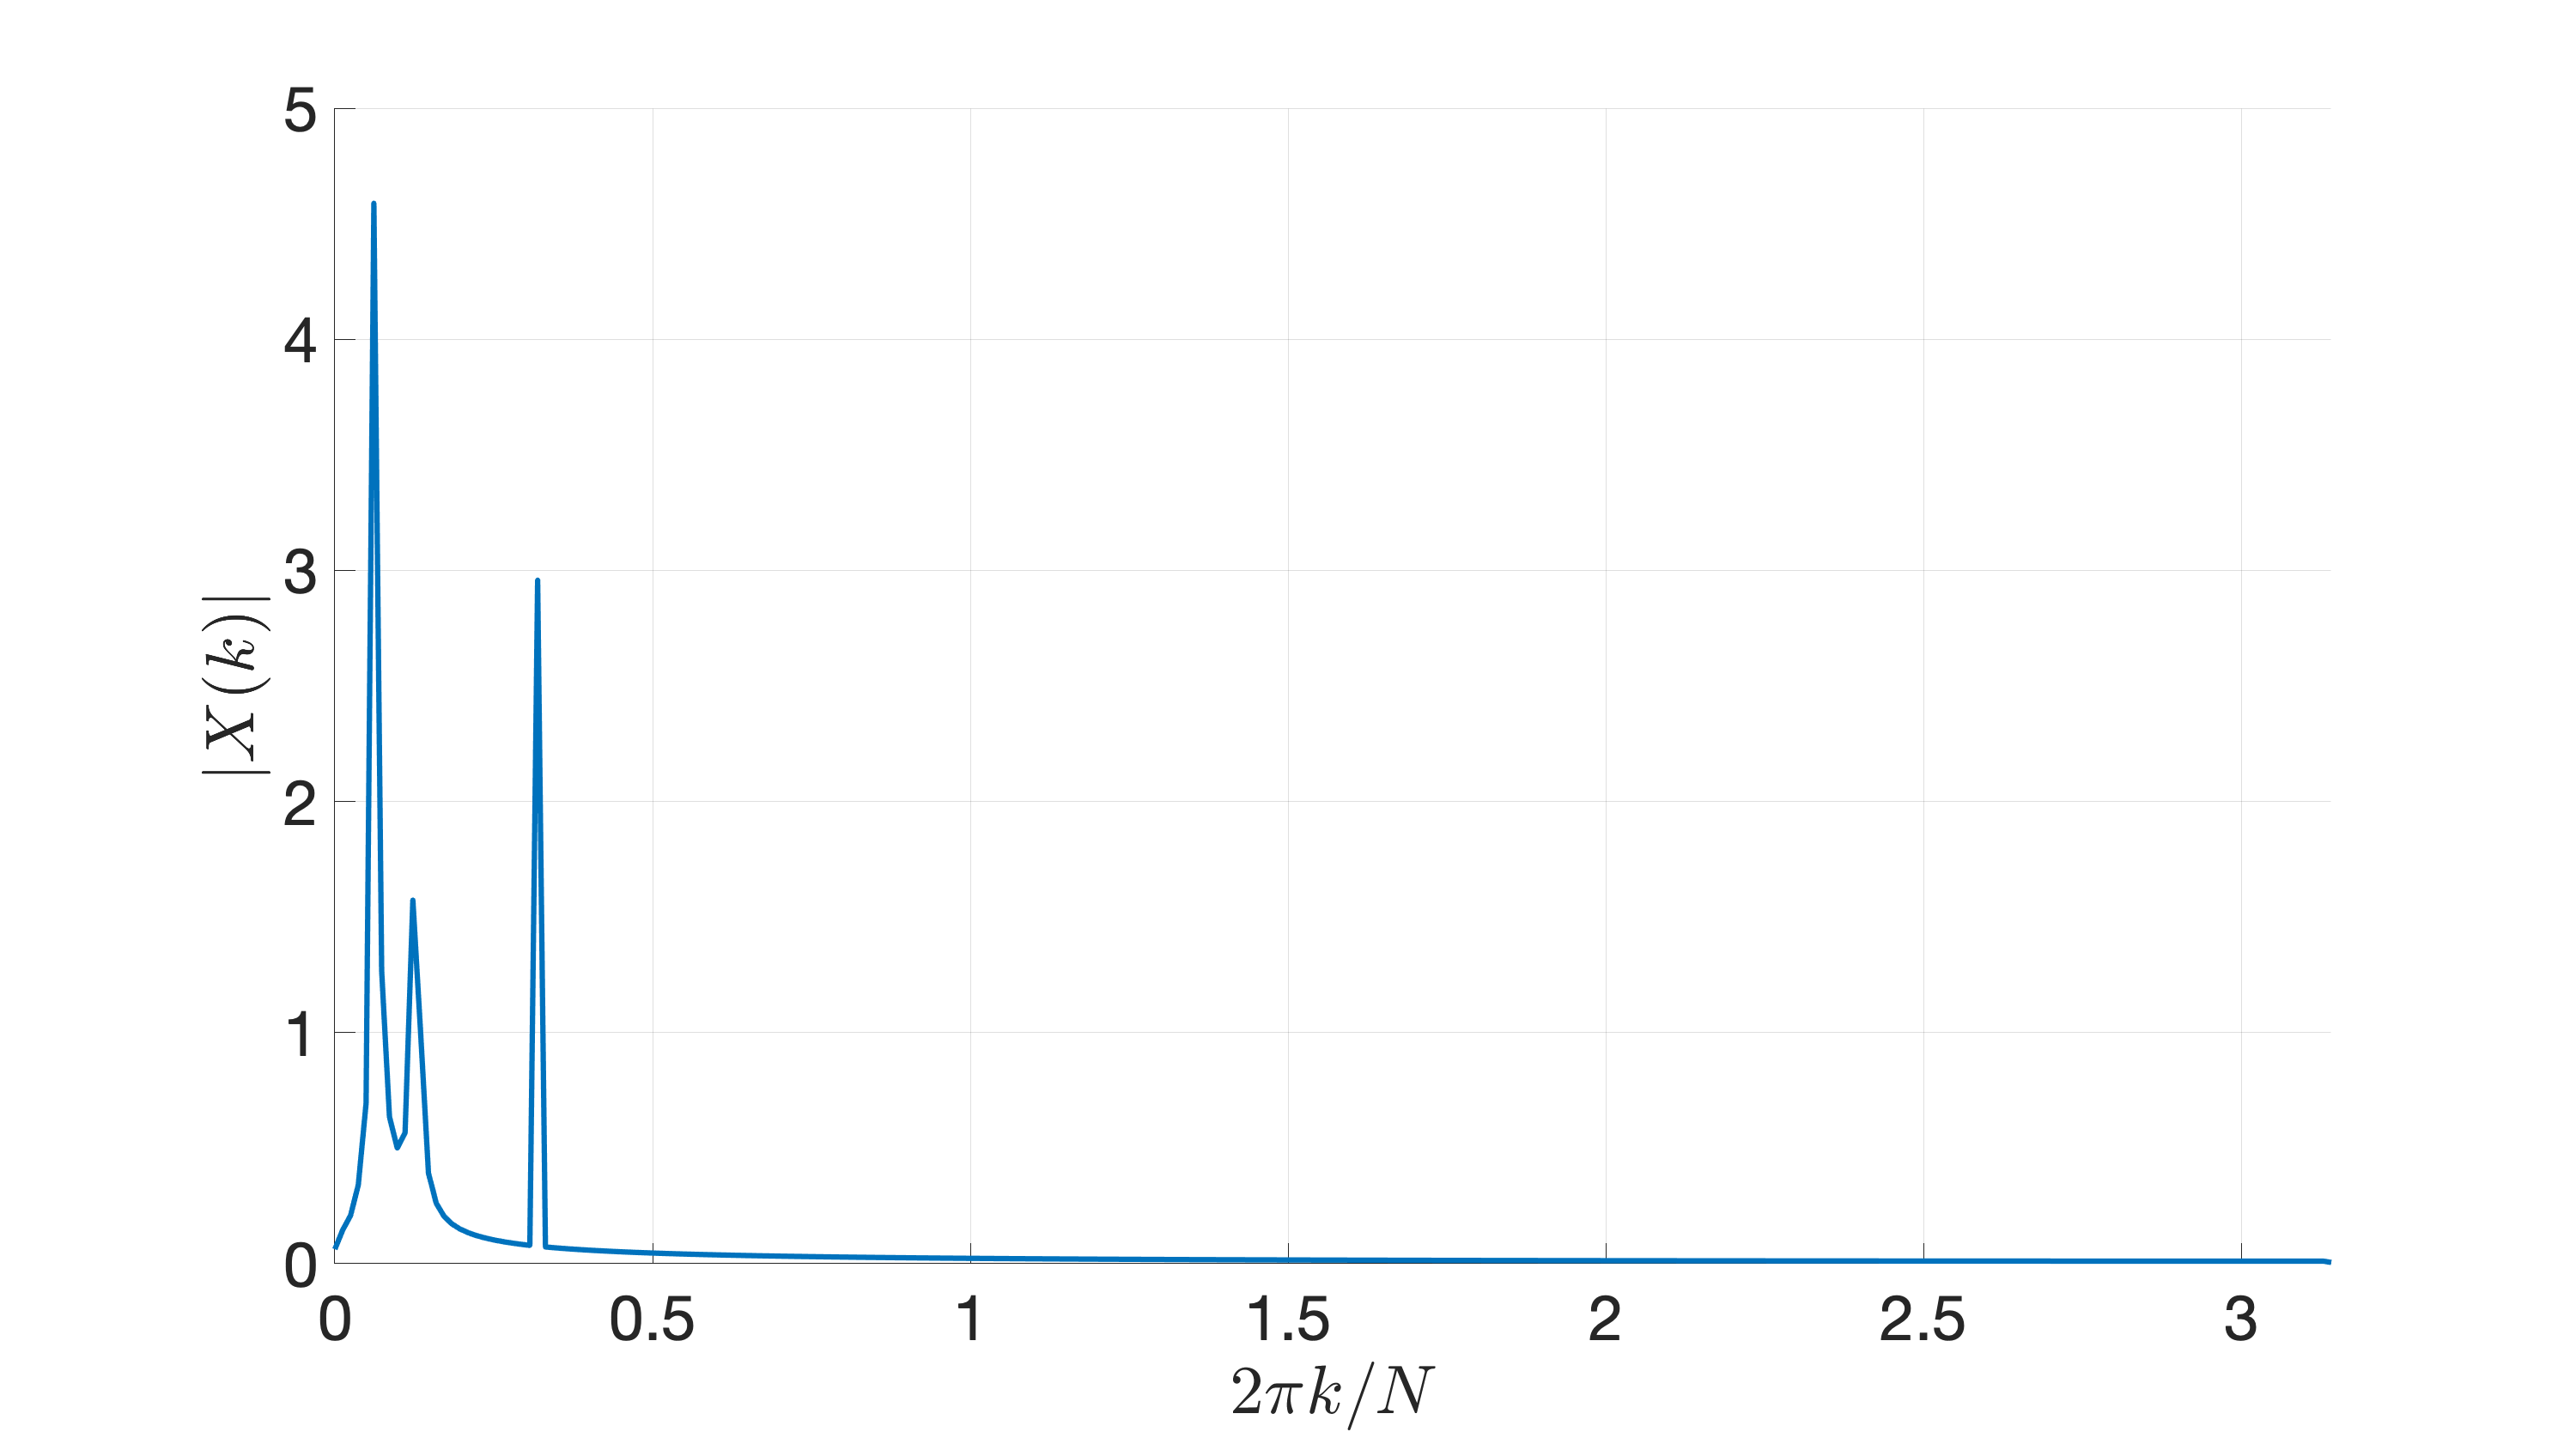
\includegraphics[width= 0.8\textwidth]{figures/R1c_mag.png}
	\caption{Magnitude of the one-sided DFT coefficients as a function of the normalized frequency.}
	\label{fig:R1c_mag}
\end{figure}
\begin{figure}[htbp]
	\centering
	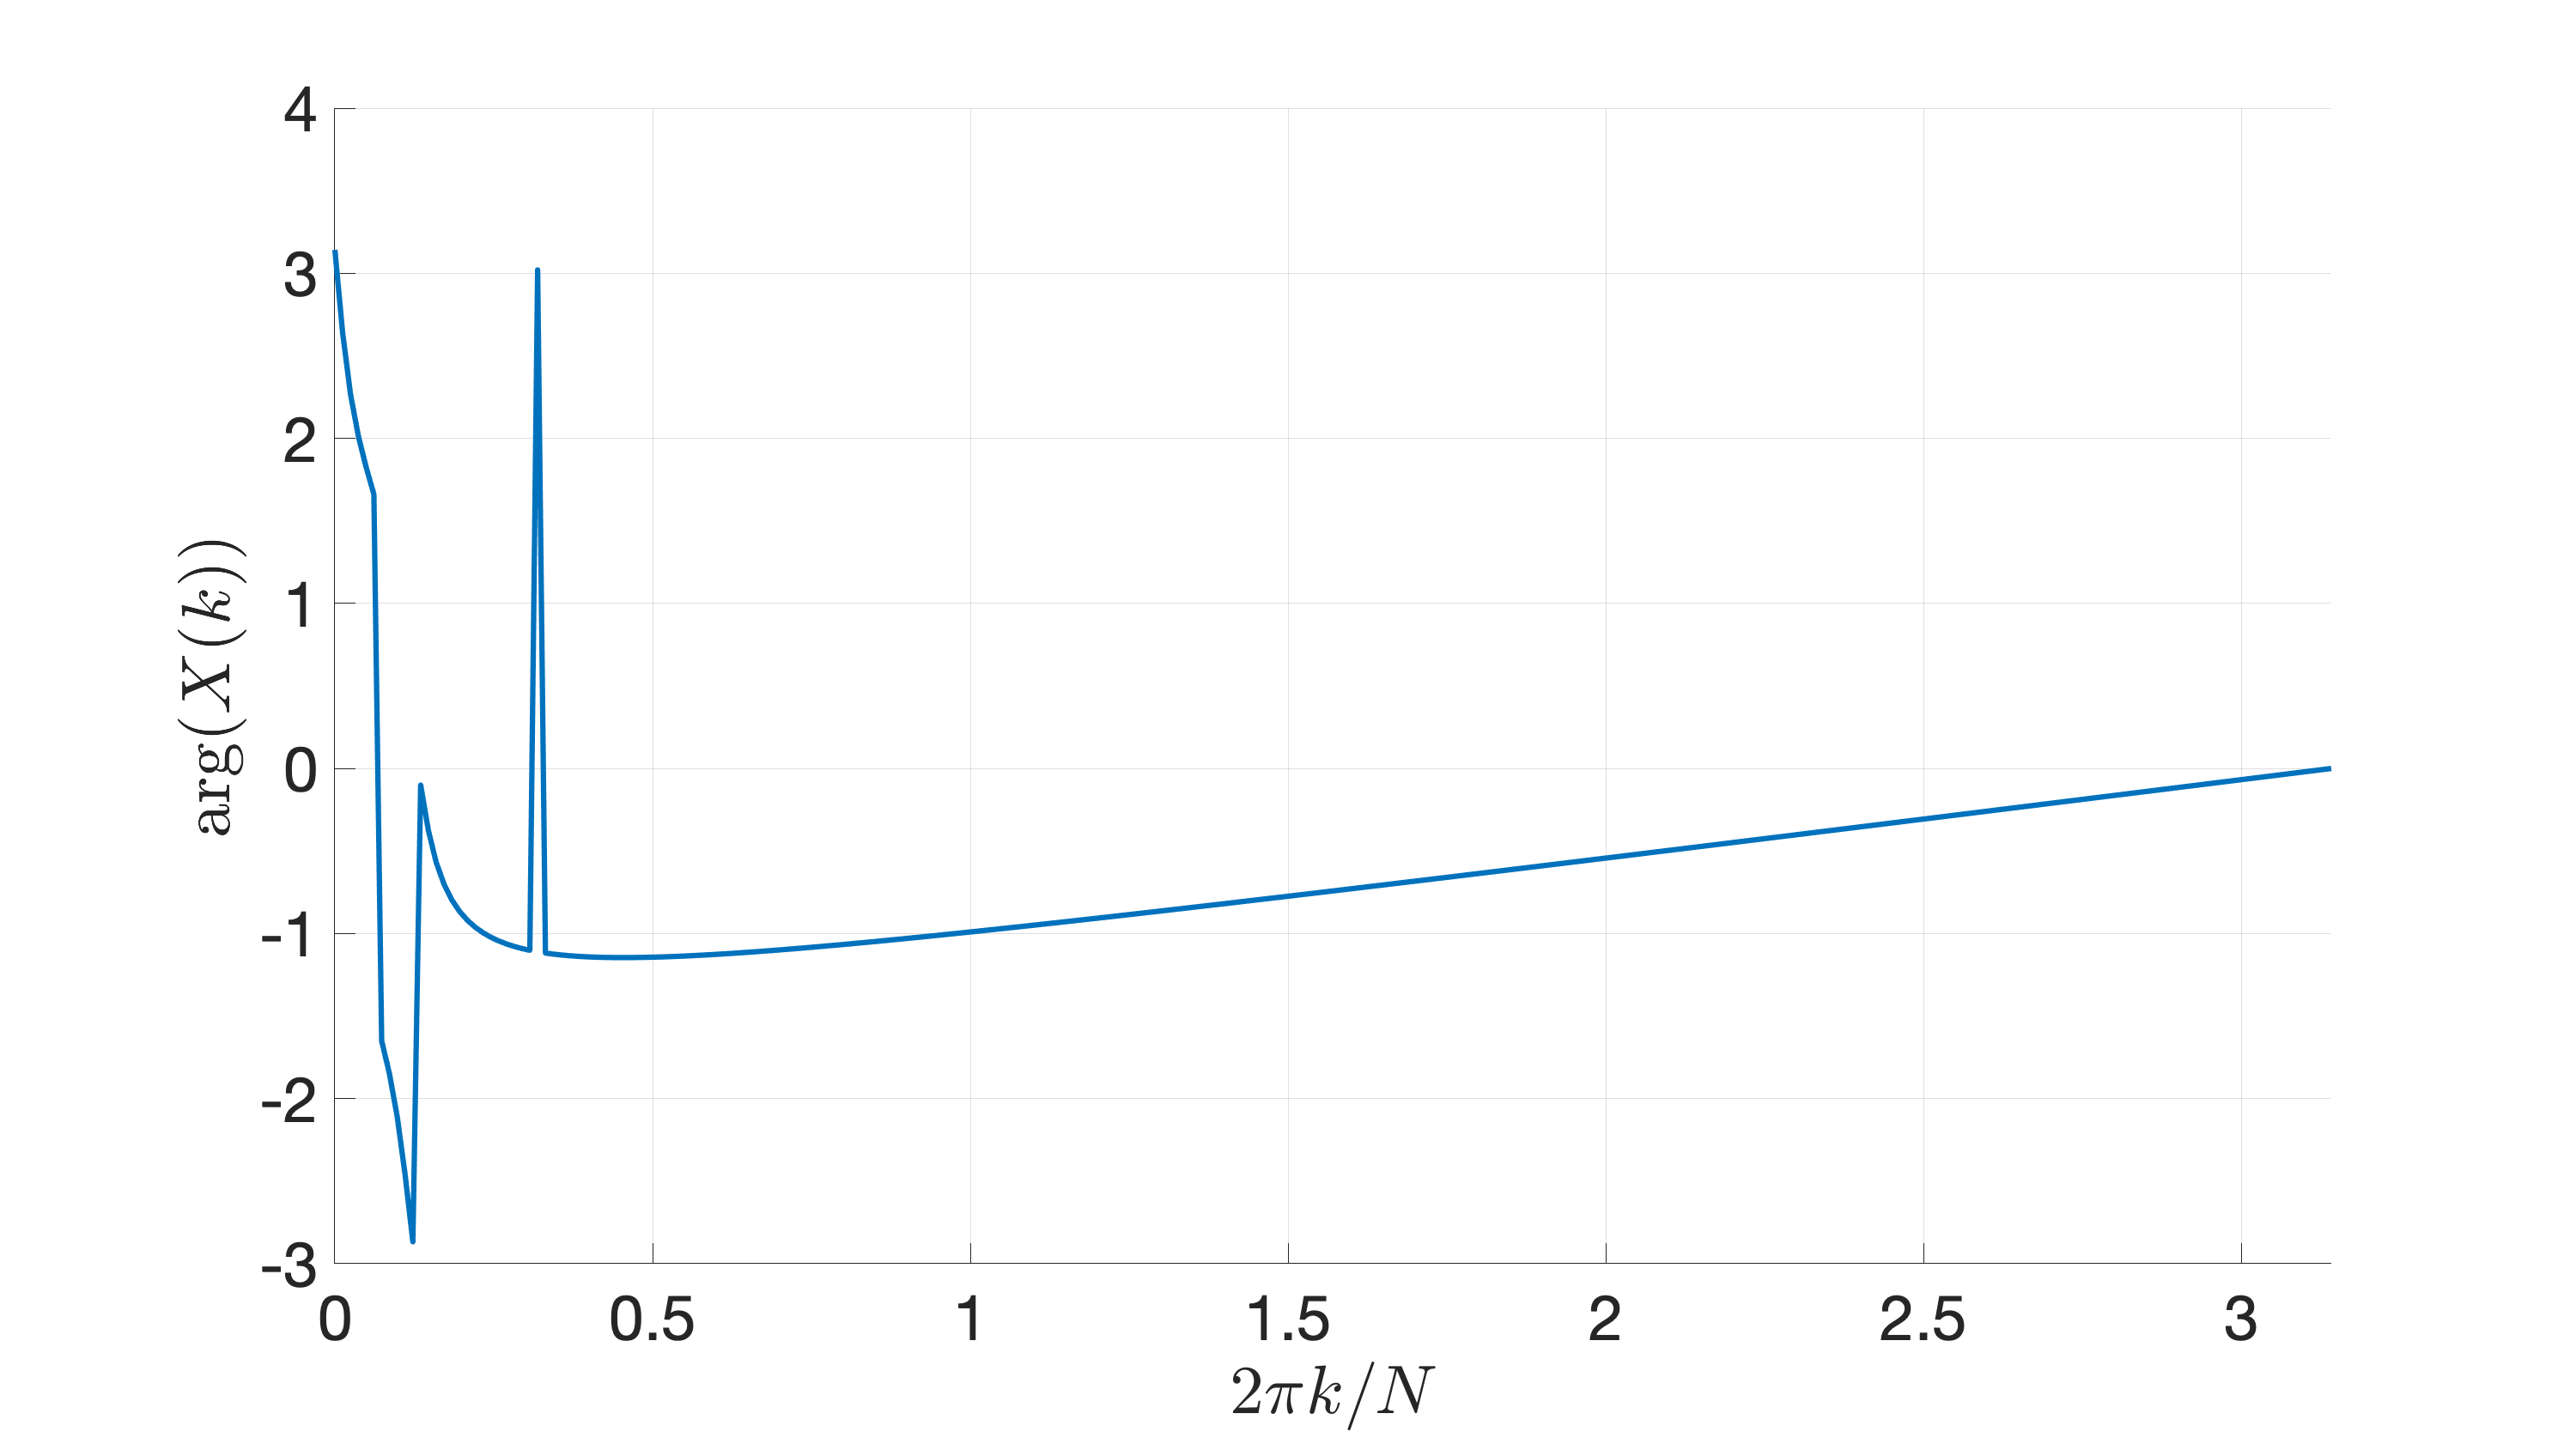
\includegraphics[width= 0.8\textwidth]{figures/R1c_arg.png}
	\caption{Argument of the one-sided DFT coefficients as a function of the normalized frequency.}
	\label{fig:R1c_arg}
\end{figure}

\subsection{R1.d) Peaks of the magnitude of the DFT coefficients}
The index $k$, normalized frequency $\omega(k)$, magnitude $|X(k)|$, and argument $\mathrm{arg}(|X(k)|)$ of one-sided DFT coefficients corresponding to the peaks of Fig. \ref{fig:R1c_mag} are shown in Table \ref{tb:peaks}.

\begin{table}[htbp]
	\centering
	\caption{One-sided DFT coefficients corresponding to the peaks of Fig.\ref{fig:R1c_mag}.}
	\label{tb:peaks}
	\begin{tabular}{cccc}
		\hline
		$k$ & $\omega(k) \: (\mathrm{rad\:s^{-1}})$ & $|X(k)|$ & $\mathrm{arg}(|X(k)|)\: (\mathrm{rad})$\\
		\hline
		5 & $2\pi k/N \approx 0.0614$ & $ 4.5886$ & 1.6611\\
		10 & $2\pi k/N \approx 0.1227$ & $ 1.5735$ & -2.8673  \\
		26  & $2\pi k/N \approx 0.3191$ & $ 2.9577$ & 3.0211 \\
		\hline
	\end{tabular}
\end{table}

It is important to remark that none of the the two lowest frequency harmonics of the original signal $x(n)$ are an integer multiple of $2\pi /N$. As a result, the normalized frequencies of the corresponding peaks of the one-sided DFT do not exactly correspond to the frequencies of the harmonics of the original signal. On the other hand, the frequency of the third harmonic $5\omega_0$ can be written as $26\times2\pi/N$, thus the normalized frequency of the peak should match the frequency of the harmonic. Furthermore, albeit not exactly equal, the normalized frequencies, magnitude, and argument of the one-sided DFT coefficients are very close to those of the harmonics of the original signal, as it can be seen in Table \ref{tb:comp_peaks}. The closest, as expected, is the highest frequency harmonic.

\begin{table}[htbp]
	\centering
	\caption{One-sided DFT coefficients corresponding to the peaks of Fig.\ref{fig:R1c_mag}.}
	\label{tb:comp_peaks}
	\begin{tabular}{cc|cc|cc}
		\hline
		 $\omega$ & $\omega(k) \: (\mathrm{rad\:s^{-1}})$ & Amplitude & $|X(k)|$ & Phase & $\mathrm{arg}(|X(k)|)\: (\mathrm{rad})$\\
		\hline
		$\omega_0 \approx 0.0638$  & $2\pi k/N \approx 0.0614$ & 5 & $ 4.5886$ & 1 & 1.6611\\
		$2\omega_0 \approx 0.1276$ & $2\pi k/N \approx 0.1227$ & 2 & $ 1.5735$ & 2 & -2.8673  \\
		$5\omega_0 \approx 0.3191$ & $2\pi k/N \approx 0.3191$ & 3 & $ 2.9577$ & 3 & 3.0211 \\
		\hline
	\end{tabular}
\end{table}


\subsection{R1.e) Reconstruction of synthetic signal (N = 512)}

Third of all, the signal $x(n)$ can be reconstructed from the three peaks identified in one-sided magnitude spectrum, as the linear combination of complex exponential functions. The reconstructed signal $x_r(n)$ is shown and compared with the original signal in \ref{fig:R1e}. It is visible that, although it accurate in the frequency domain, it is not able to reproduce the original signal very accurately in the time domain. The sum of the squared errors amounts to $SSE \approx 1224.5$.

\begin{figure}[htbp]
	\centering
	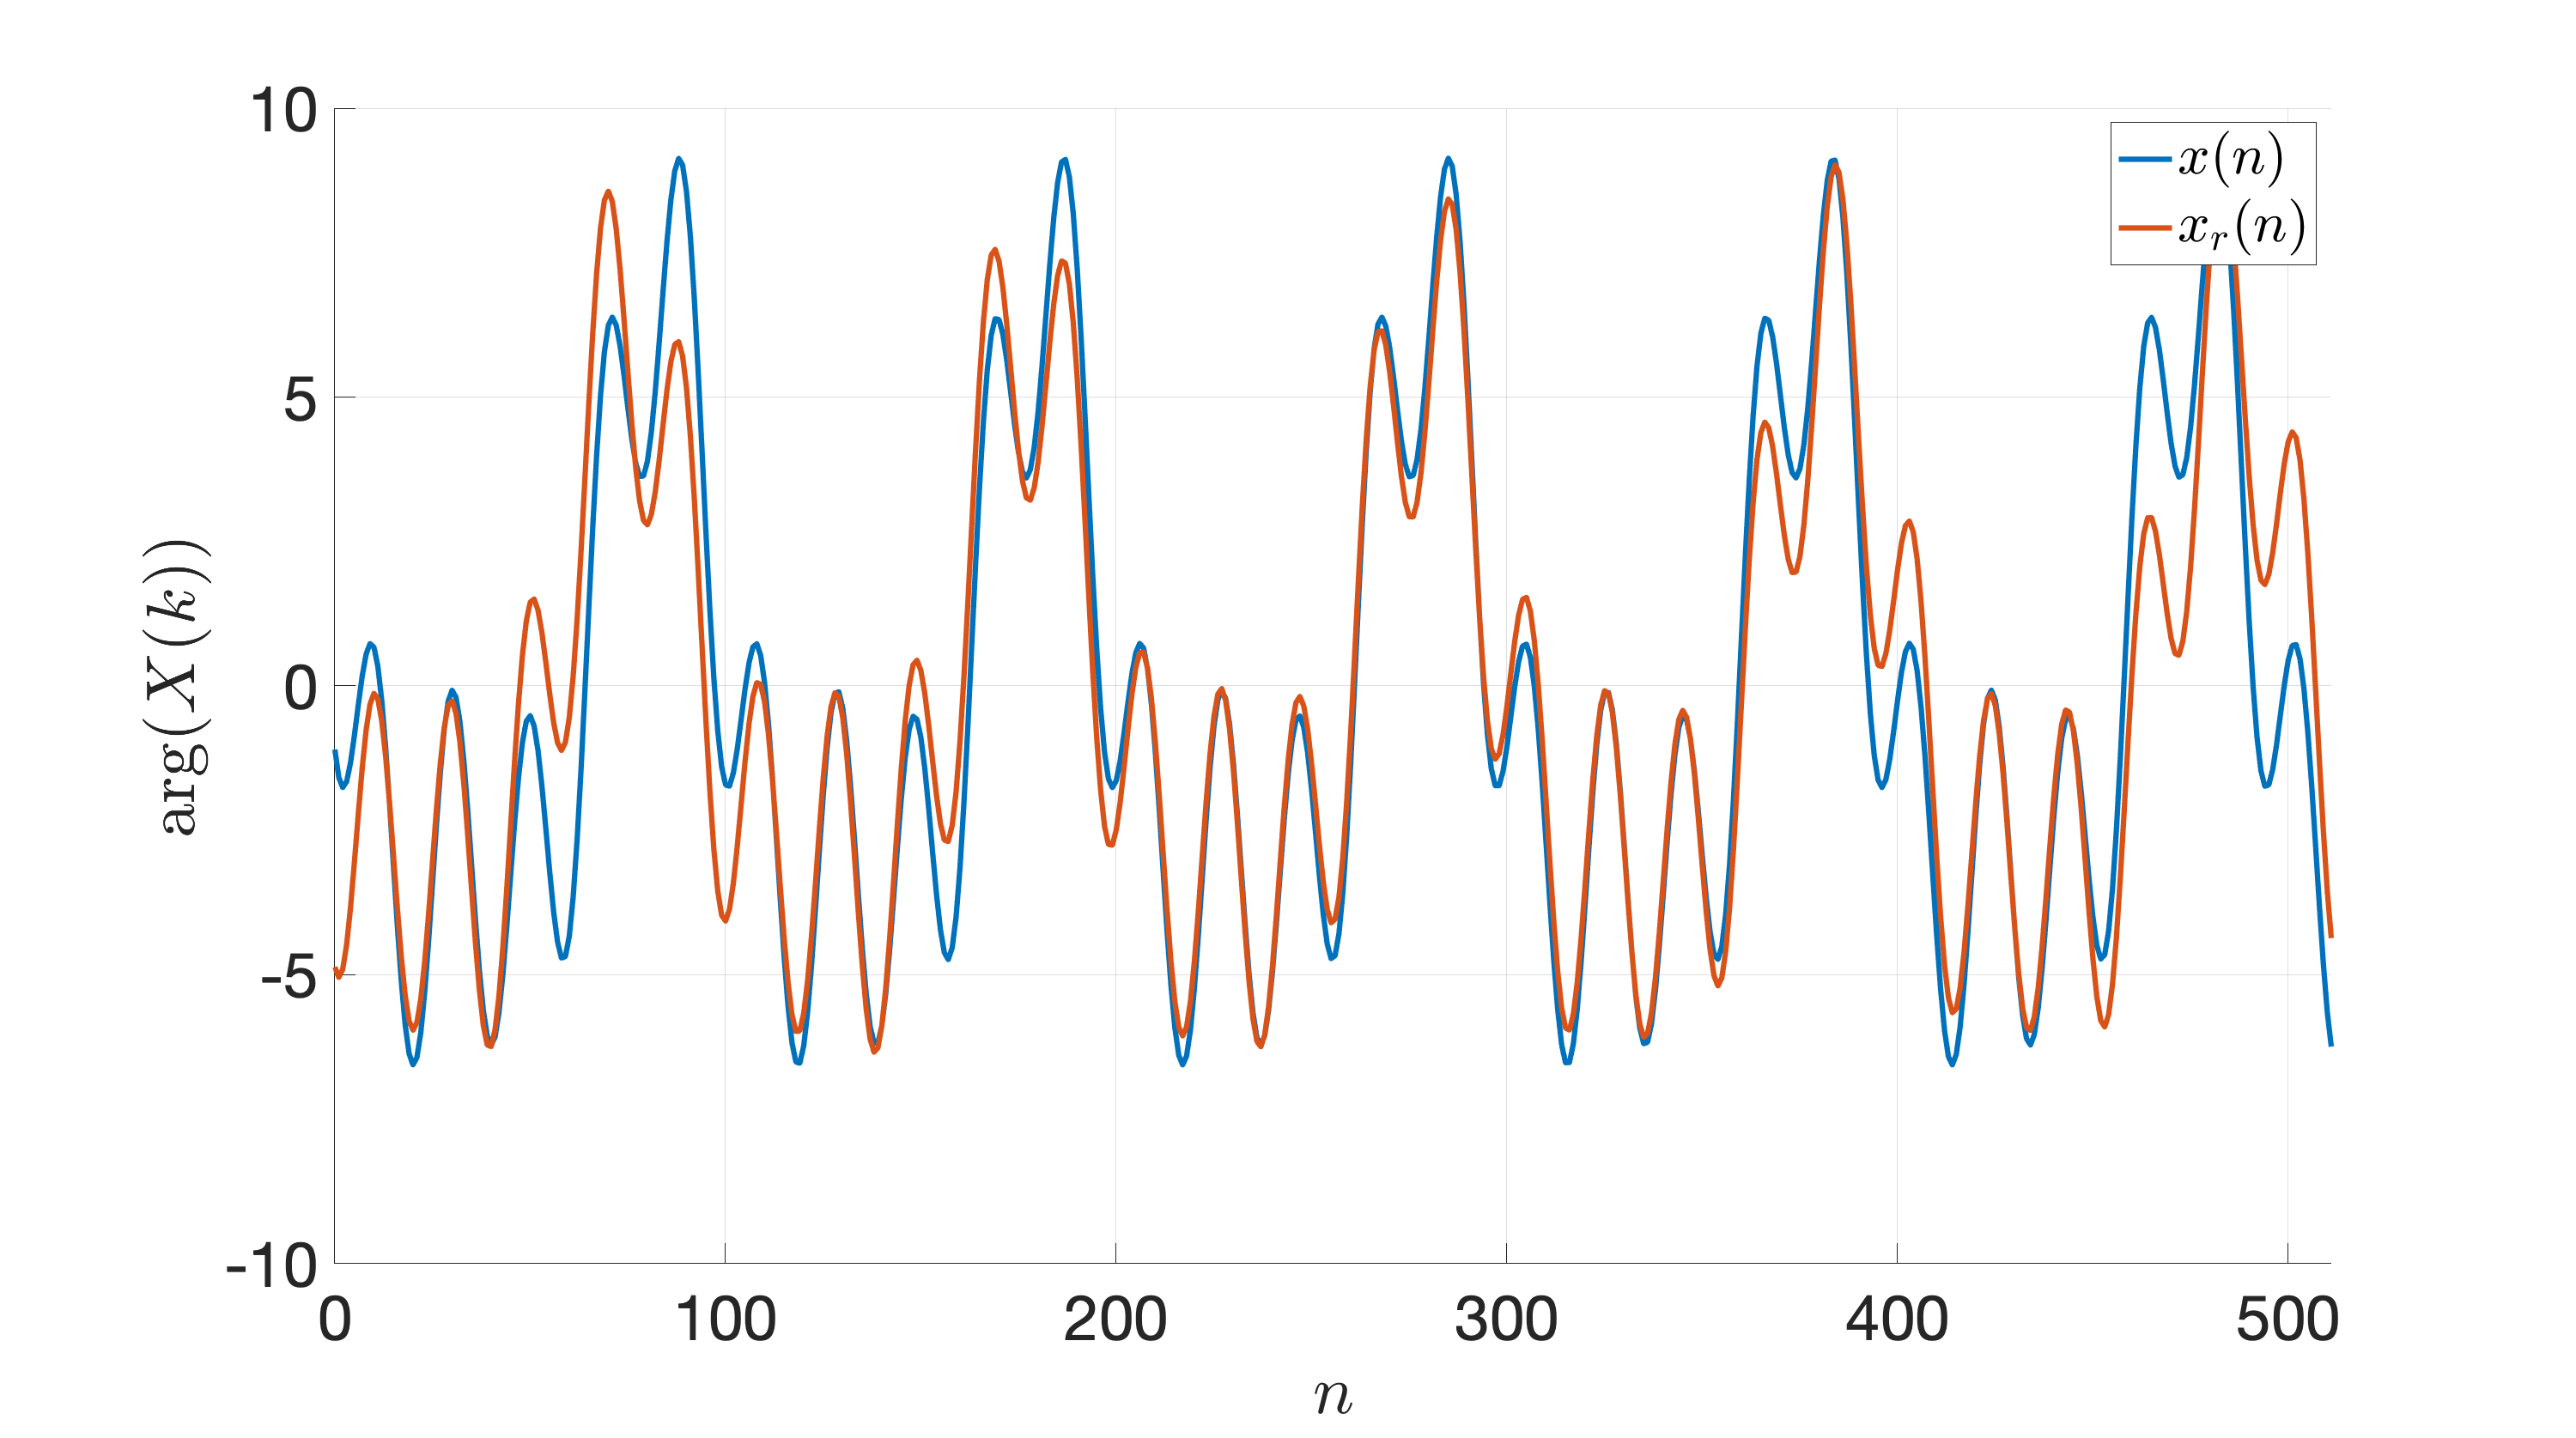
\includegraphics[width= 0.8\textwidth]{figures/R1e.png}
	\caption{Comparison between the reconstructed signal and the original, for $N = 512$.}
	\label{fig:R1e}
\end{figure}

\subsection{R1.f) Reconstruction of synthetic signal (N = 1024)}

Fourth of all, the DFT the original signal was performed with a window length of $N= 1024$. The increase of the DFT length allows to have double the precision on the normalized frequencies in relation to $N = 512$. As a result the three largest peaks identified in the one-sided magnitude spectrum of the DFT are presented in Table \ref{tb:peaks_N}. Note that, only the harmonic of frequency $2\omega_0$ as identified with more precision, as the increase of precision is not great enough to notice an improvement in the lowest frequency harmonic.

\begin{table}[htbp]
	\centering
	\caption{One-sided DFT coefficients, with $N = 1024$, corresponding to the three largest peaks of the magnitude spectrum.}
	\label{tb:peaks_N}
	\begin{tabular}{cccc}
		\hline
		$k$ & $\omega(k) \: (\mathrm{rad\:s^{-1}})$ & $|X(k)|$ & $\mathrm{arg}(|X(k)|)\: (\mathrm{rad})$\\
		\hline
		10 & $2\pi k/N \approx 0.0614$ & $ 4.5886$ & 1.6611\\
		21 & $2\pi k/N \approx 0.1289$ & $ 1.5735$ & 1.6176 \\
		52  & $2\pi k/N \approx 0.3191$ & $ 2.9577$ & 3.0211 \\
		\hline
	\end{tabular}
\end{table}


The signal $x(n)$ can, again, be reconstructed from the three peaks identified in one-sided magnitude spectrum, as the linear combination of complex exponential functions. The reconstructed signal $x_r(n)$ is shown and compared with the original signal in \ref{fig:R1f}. Comparing Figs. \ref{fig:R1e} and \ref{fig:R1f}, it is visible that it is able to reproduce the original signal more accurately. In fact, the sum of the squared errors amounts to $SSE \approx 876.5$, which is a decrease of 28\% .

\begin{figure}[htbp]
	\centering
	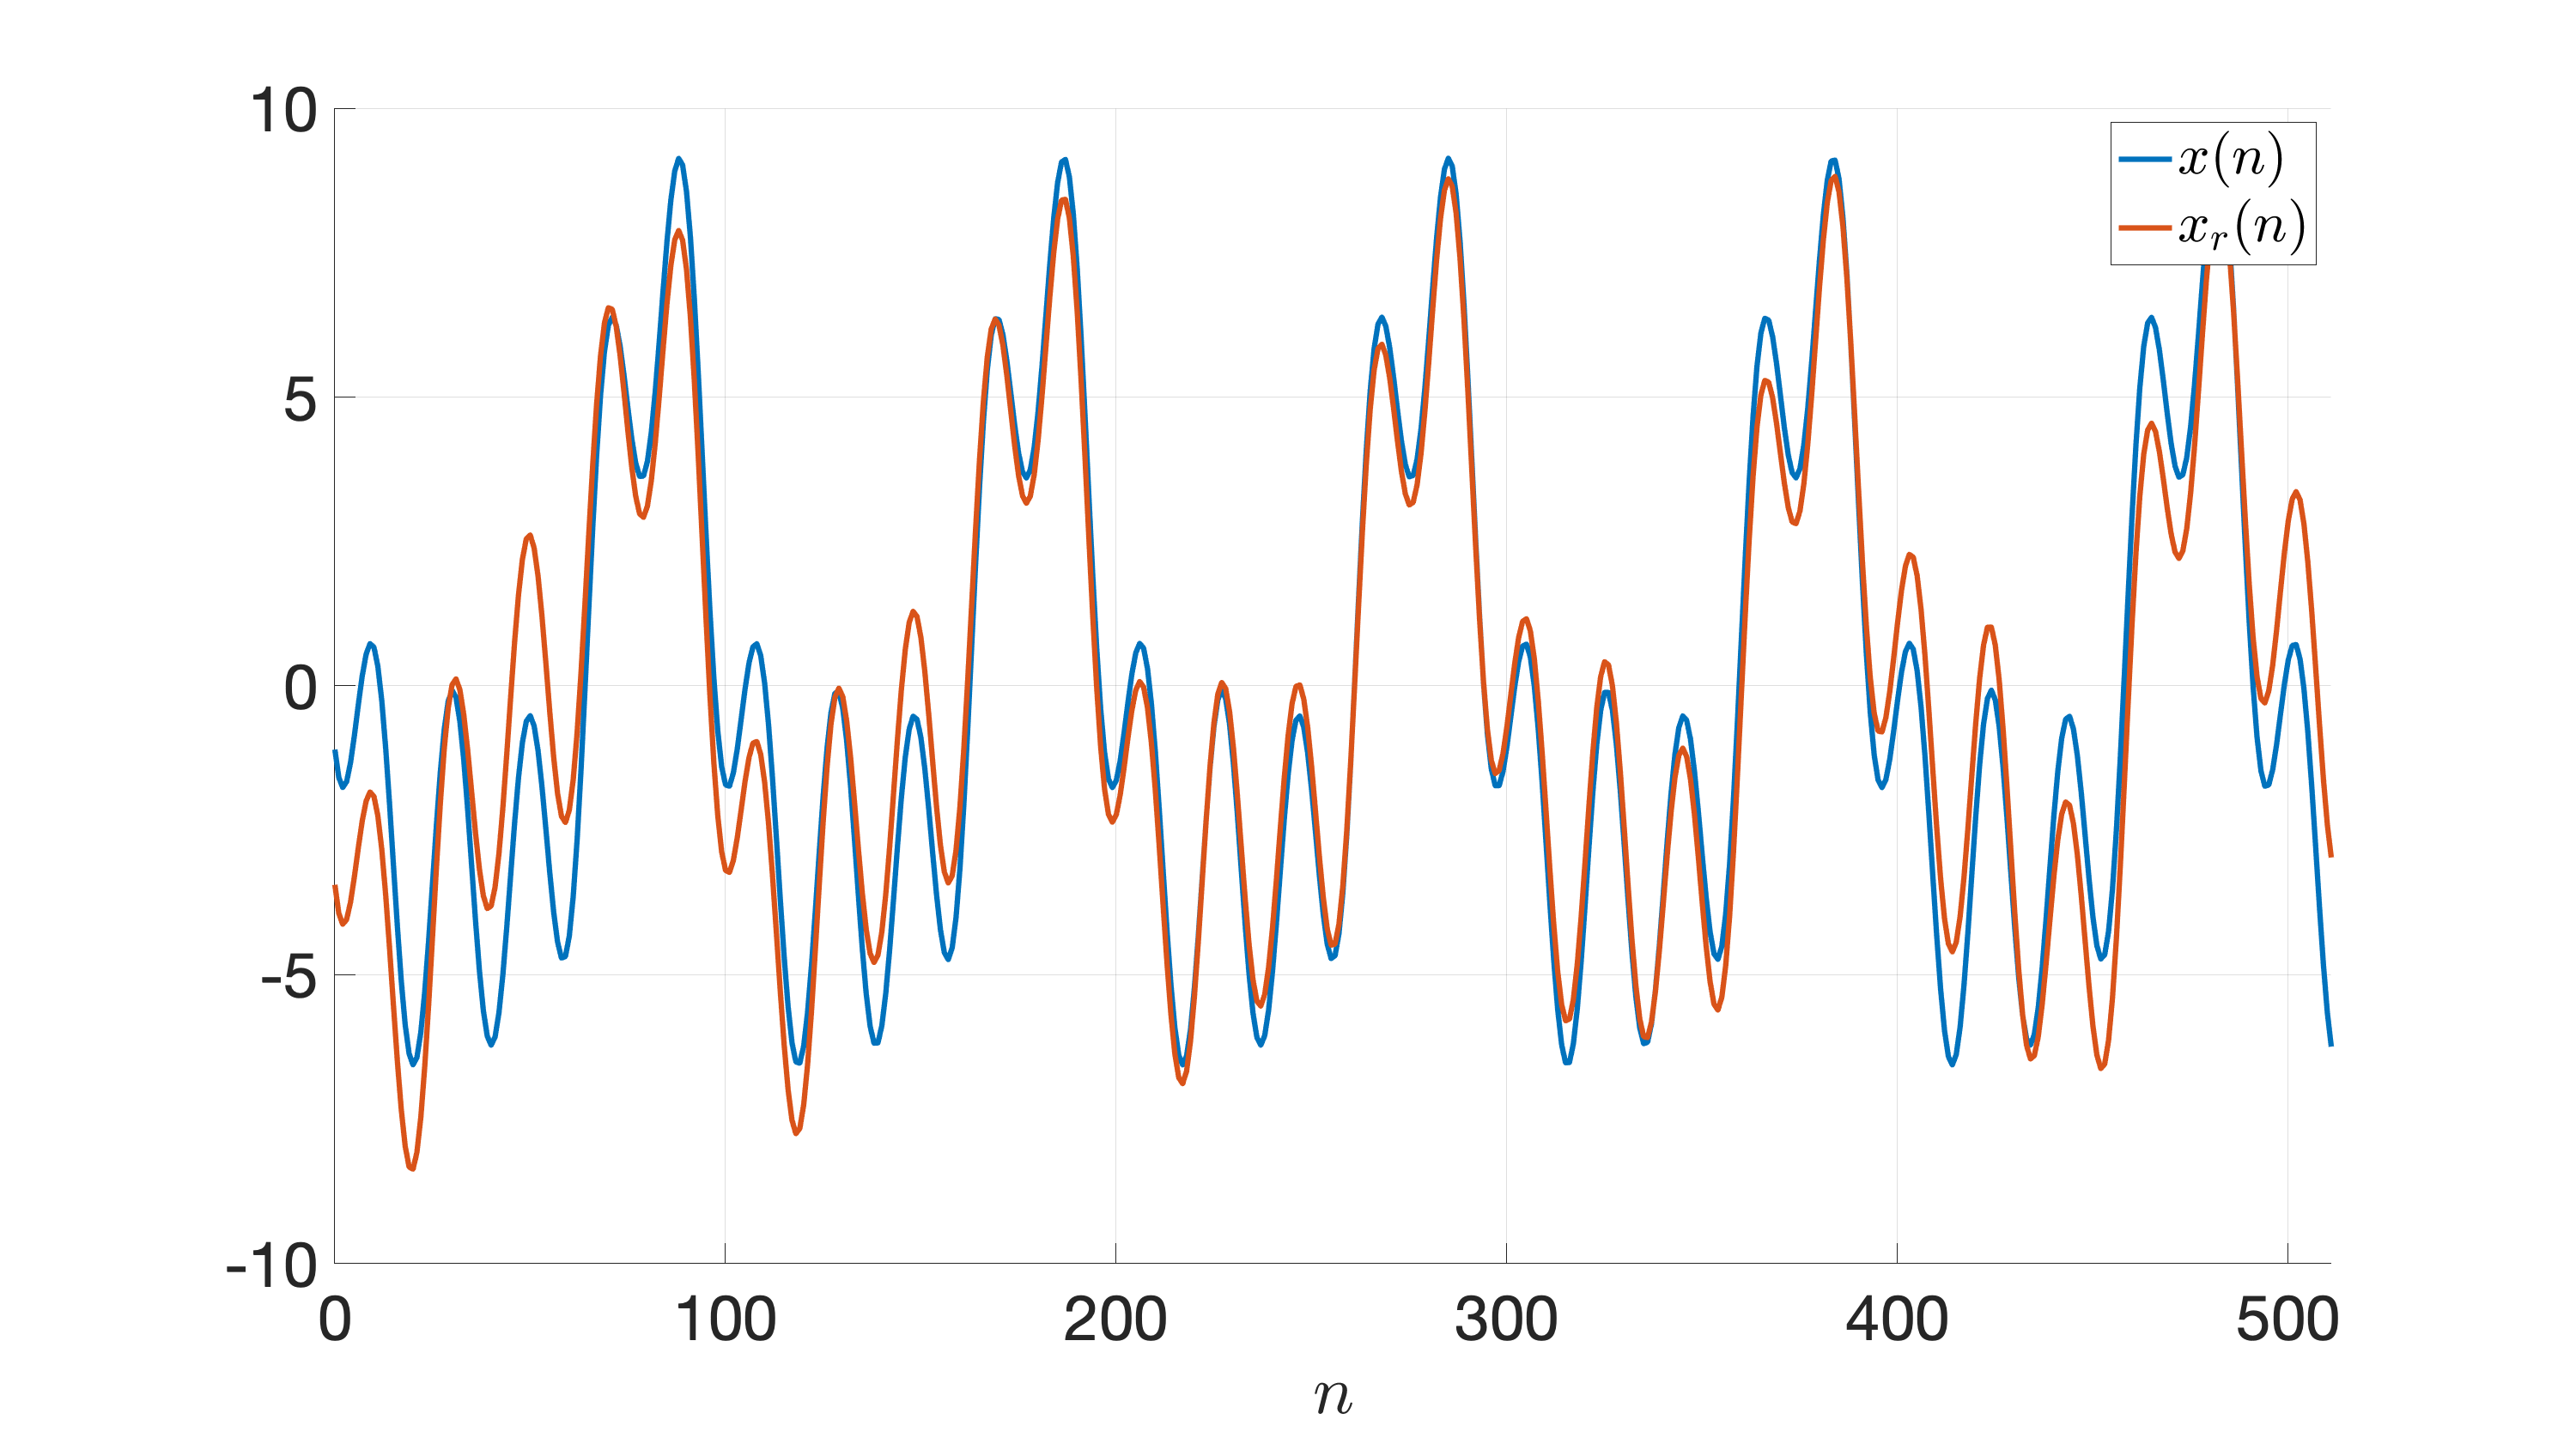
\includegraphics[width= 0.8\textwidth]{figures/R1f.png}
	\caption{Comparison between the reconstructed signal and the original, for $N = 1024$.}
	\label{fig:R1f}
\end{figure}

Furthermore, as pointed out in Section \ref{sec:R1a}, the angular frequency of the lowest harmonic can be written as an irreducible rational fraction of $2\pi$ as $\omega_0 = 2\pi \times 13/1280$. Thus, in order to identify the angular frequencies of all the harmonics exactly, a DFT of length $N = 1280$ is required. As a curiosity, such DFT was performed and the reconstructed signal from the three highest peaks in the one-sided magnitude spectrum is presented in Fig. \ref{fig:R1f_1280}. It is visible that it is able to reproduce the original signal very accurately in the time-domain, achieving $SSE \approx 11.6$.

\begin{figure}[htbp]
	\centering
	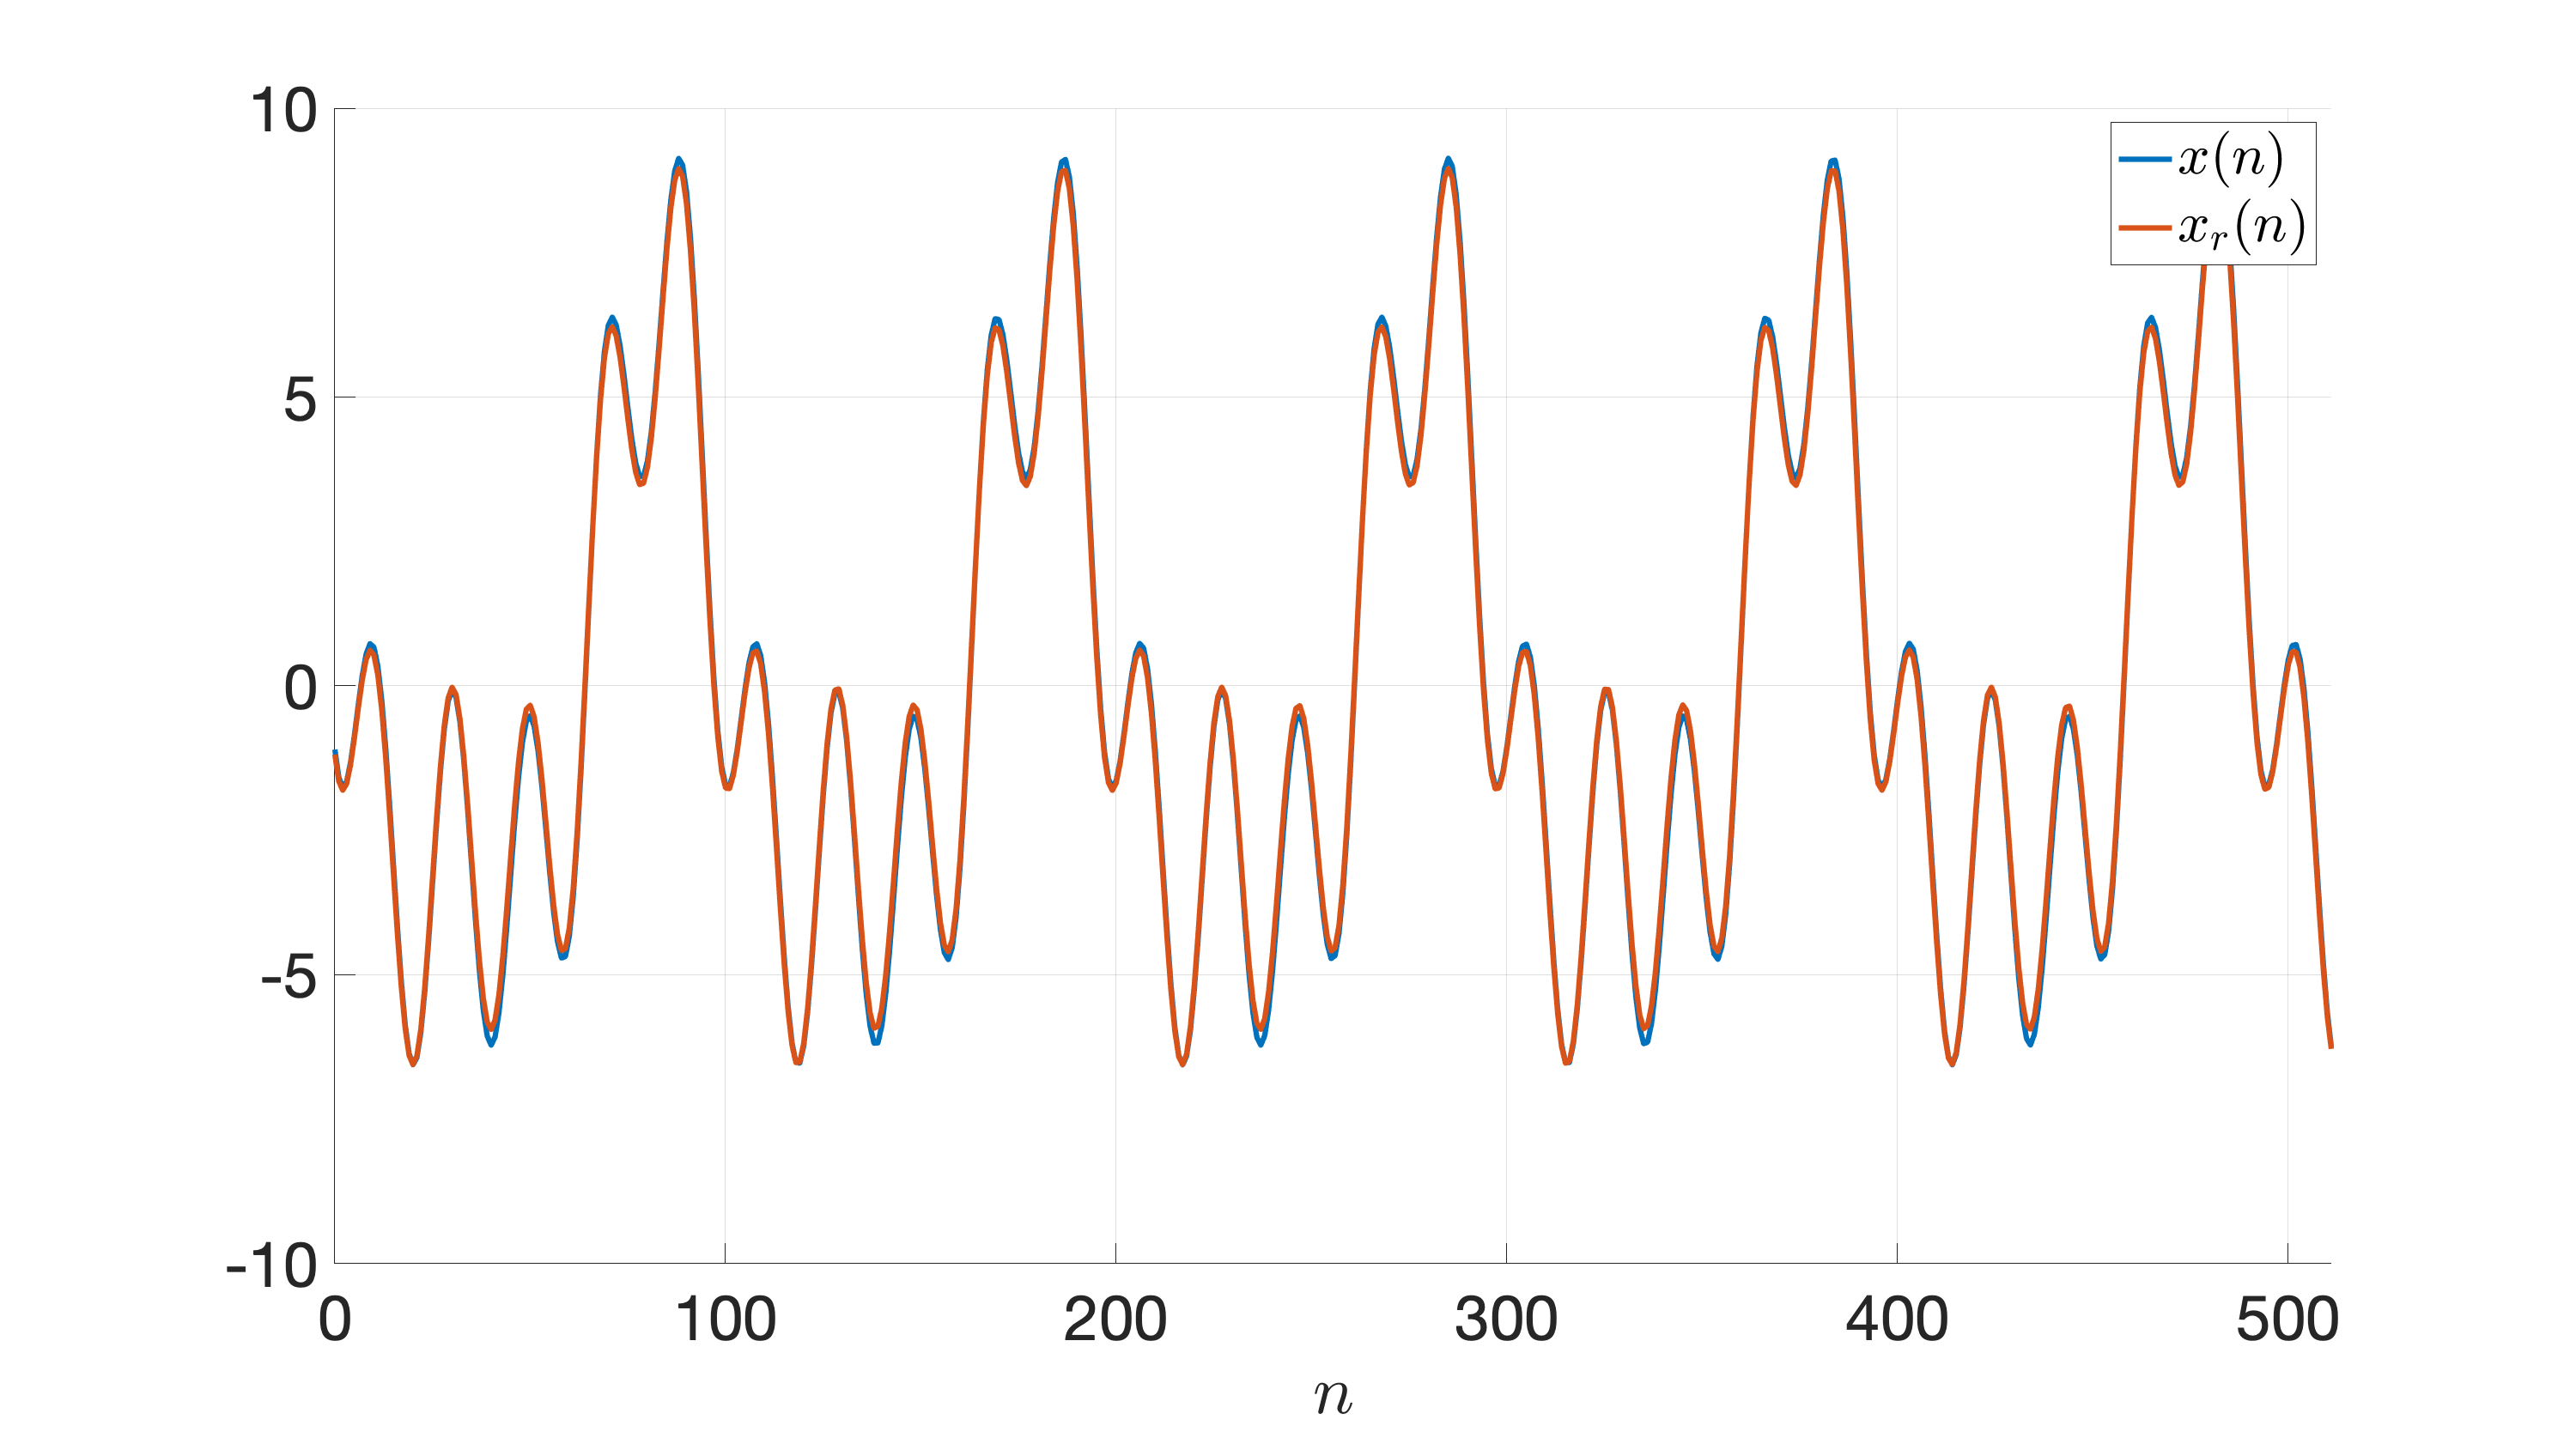
\includegraphics[width= 0.8\textwidth]{figures/R1f_1280.png}
	\caption{Comparison between the reconstructed signal and the original, for $N = 1280$.}
	\label{fig:R1f_1280}
\end{figure}

\end{comment}

\end{document}
